%!TEX TS-program = xelatex
%!TEX encoding = UTF-8 Unicode

% Load Thesis Class
\documentclass{DEIThesis}
\usepackage{multirow}
\usepackage[toc]{appendix}
\usepackage{xcolor}
\usepackage{xltabular}

\title{Knowledge Graph Fact Verification using Retrieval-Augmented Generation}

\author{Farzad Shami}
\studentId{2090160}

% Advisor
\advisor{Prof. Gianmaria Silvello}

% If you are co-advised
\coadvisor{Prof. Stefano Marchesin}
\coadvisorsUniversity{University of Padova}

\university{University of Padova}
\departmentname{Department of Information Engineering}
\mastername{Computer Engineering}


\academicYear{2024/2025}
\gradutionDate{nth March 2025}

\begin{filecontents*}[overwrite]{\jobname.xmpdata}
    \Title{Knowledge Graph Fact Verification using Retrieval-Augmented Generation}
    \Author{Farzad Shmai}
    \Language{en-EN}
    \Keywords{Computer Engineering\sep LaTeX}
\end{filecontents*}

% Document

\begin{document}
    % Add a period to the end of an abbreviation unless there's one
    \makeatletter
    \DeclareRobustCommand\onedot{\futurelet\@let@token\@onedot}
    \def\@onedot{\ifx\@let@token.\else.\null\fi\xspace}

    \def\eg{\emph{e.g}\onedot} \def\Eg{\emph{E.g}\onedot}
    \def\ie{\emph{i.e}\onedot} \def\Ie{\emph{I.e}\onedot}
    \def\cf{\emph{c.f}\onedot} \def\Cf{\emph{C.f}\onedot}
    \def\etc{\emph{etc}\onedot} \def\vs{\emph{vs}\onedot}
    \def\wrt{w.r.t\onedot} \def\dof{d.o.f\onedot}
    \def\etal{\emph{et al}\onedot}
    \makeatother
    % The front matter (Cover, ToC, Abstract, etc...)
    \frontmatter

    % The main content
    \mainmatter
    
    \chapter{Introduction}\label{ch:intro}
\acp{KG} have become an indispensable component of modern information systems and are widely used in different categories, including search engines~\cite{google_knowledge_graph}, recommendation systems~\cite{guo2020surveyknowledgegraphbasedrecommender}, and question-answering platforms~\cite{omar2023universalquestionansweringplatformknowledge}.
\ac{KG} is a directed, multi relational graph, which represents entities as nodes and their relationships as edges, and can be used as an abstraction of the real world~\cite{ali2020keenuniverseecosystemknowledge}.
These \acp{KG} have appears as an effective tool for arranging and querying massive amounts of structured data.
Maintaining the accuracy and dependability of \acp{KG} is a significant challenge, as they have become a standard in representing factual information across different domains.
Prominent examples of KGs are DBpedia~\cite{lehmann2015dbpedia}, Wikidata~\cite{10.1145/2629489}, Freebase~\cite{10.1145/1376616.1376746}, and Knowledge Vault~\cite{10.1145/2623330.2623623}.

On the other side, in the past few years, the increasing volume of online content, coupled with the rise of misinformation and disinformation, necessitate the need ways to verify the correctness of the information.
So, ensuring the truthfulness of the information is an important task to maintain the reliability in knowledge-driven applications, particularly as \ac{AI} and automated decision-making systems become more prevalent.

Considering that KGs are often incomplete and noisy, performing fact verification on \acp{KG} is a challenging task.
To evaluate the correctness of a fact, humans need to check the information against several external sources, which can be time-consuming and error-prone.
Evaluating the reliability of each source is another challenge.
This process can take even professional fact-checkers a long time to complete, and it's not always easy to know if the information is correct.
As this process is time-consuming and the amount of information is increasing day by day, we can notice that manual fact-checking is not a feasible solution.

To address these challenges, there were two types of methods in the past that automate the process of fact-checking:
(1) Statistical and rule-based techniques and (2) Sampling techniques that try to reduce the human effort in the fact-checking process by using the samples the data from datasets.
The first type of methods can work for some types of facts~\footnote{In this work, we use the terms fact, claim and triple interchangeably.}, but they don't work well for more complicated or subtle data.
The second type of methods can be more effective, but they do not check all aspects of the data, and they may not be able to verify all the facts.

In response to these limitations, the past few years have witnessed the growing adoption of \ac{ML} and \ac{NLP} techniques as new possibilities in this field.
These techniques have shown remarkable success and change the traditional methods to be more effective and somehow automatic.
With advances in \ac{NLP} and the emergence of \acp{LLM}, the fact-checking process changed dramatically.

\acp{LLM} have shown remarkable capabilities in understanding and generating human-like text, making them well-suited for tasks that require reasoning and understanding of textual information.
However, \acp{LLM} have some limitations, such as (1) hallucination, where they generate plausible but incorrect information;
(2) training data cut-off, where they are limited to the data they were trained on, which may become outdated over time;
(3) reliability of training data, where the models may not be able to verify the correctness of the information they generate;
and (4) the models contain significant information in their parameters, but their performance is not as good as task-specific architectures.
To address these limitations, researchers have proposed combining \acp{LLM} with external information retrieval to improve the accuracy and reliability of fact verification and named this technique \ac{RAG}~\cite{lewis2021retrievalaugmentedgenerationknowledgeintensivenlp}.

By combining the strengths of \acp{LLM} with external information, we introduce a novel system for automated fact verification in \acp{KG} using \ac{RAG}.
In this thesis, we introduce \texttt{FactCheck}, a system that employs a multi-model ensemble approach by merging the outputs of different LLMs through majority voting to verify facts in KGs.

\newpage
\section{Problem Statement}\label{sec:problem}
This thesis tackles the issue of automated fact verification in \acp{KG} with a RAG-based methodology.
Our objective is to create a system capable of
(1) Retrieve relevant information from external sources to support or refute claims in a \ac{KG};
(2) Utilize \acp{LLM} to reason about the retrieved information and generate accurate assessments of fact truthfulness;
(3) Handle a wide range of fact types and domains, from simple statements to more complex relational facts;
and finally (4) Using multiple \acp{LLM}, provide multiple responses for its verification decisions, enhancing transparency and trust in the system.


\section{Proposed System}\label{sec:approach}
Our proposed system combines several key components to create a fact verification system as you can see the overview in Figure~\ref{fig:factcheck-overview}.
\begin{figure}[ht!]
    \centering
    \begin{minipage}[b]{\textwidth}
        \centering
        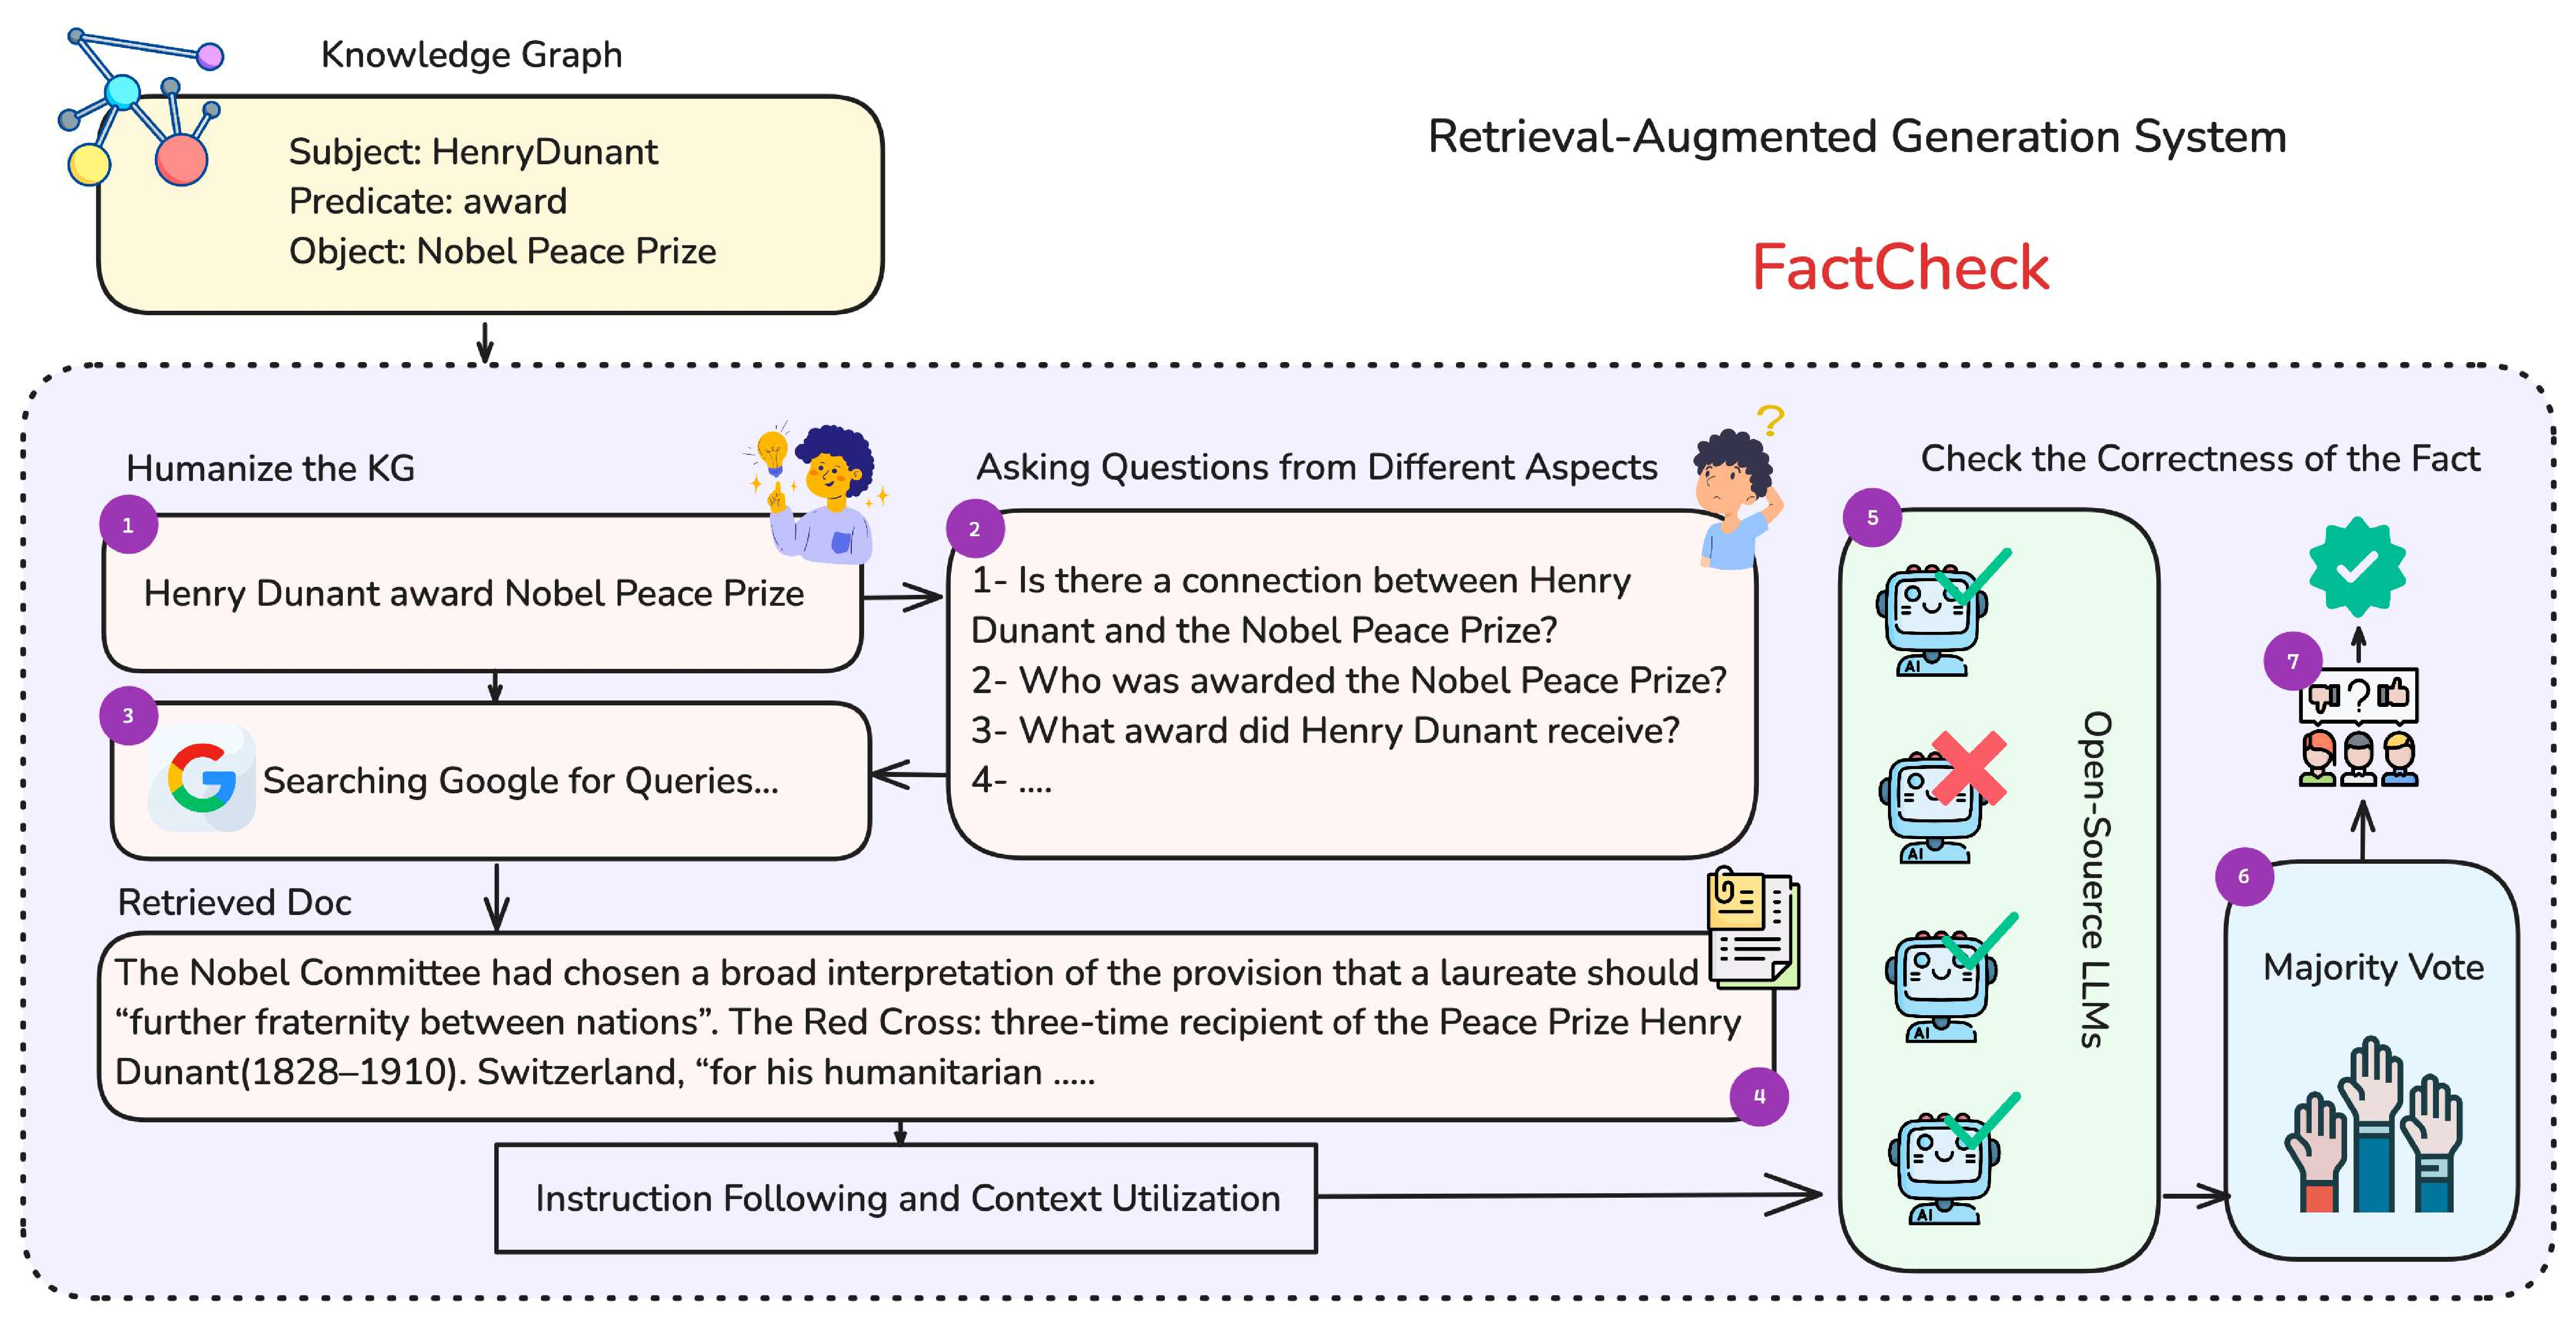
\includegraphics[width=\textwidth]{res/FactCheckOverview}
        \caption{Overview of the FactCheck system for fact verification. The system processes a knowledge graph triple through multiple stages: (1) \ac{KG} humanization, converting structured data into natural language; (2) Generation of aspect-specific questions to probe the fact; (3) Google search retrieval based on generated questions; (4) Analysis of retrieved documents containing relevant information; (5) Deployment of multiple \ac{LLMs} as open-source fact-checkers; (6) Final fact verification through majority voting; and (7) tie-breaker module.}
        \label{fig:factcheck-overview}
    \end{minipage}
\end{figure}
\newpage

The general idea behind the FactCheck system is as follows:
\begin{itemize}
    \item \textbf{\ac{KG} Representation:} We start by representing facts from the \ac{KG} in a format suitable for processing by language models and \ac{IR} systems. This involves converting the subject-predicate-object triples of the \ac{KG} into natural language statements.
    \item \textbf{Query Generation:} For each fact to be verified, we generate multiple queries designed to retrieve relevant information from external sources. These queries are formulated to capture different aspects of the fact and potential supporting or contradicting evidence.
    \item \textbf{\ac{IR}:} We use advanced \ac{IR} techniques to search for relevant documents or passages from a large corpus of trusted sources. This step leverages both traditional search algorithms and dense retrieval methods based on neural networks.
    \item \textbf{Context Processing:} The retrieved information is processed and combined to create a comprehensive context for each fact. This may involve techniques such as text summarization, entity linking, and coreference resolution to create a coherent representation of the relevant information.
    \item \textbf{\ac{LLM} Integration:} We use several \ac{LLMs} at the same time to look at the context that was retrieved and decide if the original fact is true. By putting together the results of several models, we hope to reduce the flaws in each one and make the whole thing more accurate.
    \item \textbf{Fact Verification Decision:} The system makes a final decision on the truthfulness of the fact based on the consensus of the language models and the strength of the supporting or contradicting evidence. This decision is accompanied by the reasoning process and relevant evidence.
\end{itemize}

\section{Contributions}\label{sec:contributions}
This thesis presents several significant contributions to the field of \ac{NLP} and knowledge verification systems.
Our investigation into the capabilities of \acp{LLM} within \ac{RAG} frameworks reveals their considerable potential for fact-verification tasks.
Through experimentation, we have proved that these \acp{LLM} show remarkable aptitude in adapting and contextualizing external knowledge sources which is a crucial capability for reliable information validation in contemporary applications.
By examining \acp{LLM} reasoning patterns and pathways, we provide insights into how these models arrive at verification decisions when confronted with factual claims of varying complexity.
This deeper understanding improves our theoretical grasp of these systems and suggests practical improvements for their implementation in real-world scenarios.

A particularly noteworthy aspect of this work is the assessment of computational efficiency.
Contrary to prevailing assumptions about LLMs that they require substantial computational resources, our findings indicate that effective fact-verification processes can indeed be executed on modestly provisioned local infrastructures.
This finding is important because it makes advanced AI tools more accessible to different research groups, even those with limited resources.

Finally, We conduct error taxonomy that categorizes the failure predication observed during fact-verification task.
Through this analysis, we have identified distinct error categories including context mismatches, relationship errors, role attribution discrepancies, geographic inaccuracies, and more.
This categorization exposes the current limitations of these systems and suggest ways for targeted improvements in subsequent model post-training or fine-tuning.
%
%In general, the key contributions of this work are summarized as follows:
%\begin{enumerate}
%    \item \textbf{Verification of Suitability:} We evaluate the efficacy of \ac{LLMs} in performing fact-verification tasks within \ac{RAG} frameworks, emphasizing their capability to integrate and contextualize external knowledge.
%    \item \textbf{Enhanced Understanding:} We delve into the internal mechanisms of \ac{LLMs} within the \ac{RAG} process, shedding light on their reasoning patterns and decision-making behaviors in fact-validation scenarios.
%    \item \textbf{Resource Efficiency:} We explore the feasibility of executing these procedures locally, aiming to determine whether \ac{LLMs}, often perceived as resource-intensive, can deliver high performance on computationally constrained infrastructures.
%    \item \textbf{Error Taxonomy and Analysis:} We establish a taxonomy of error types encountered in fact-verification scenarios, categorizing them as context mismatches, relationship errors, role attribution discrepancies, geographic inaccuracies, and more. This analysis provides valuable insight into the model's limitations and highlights areas for improvement in future development.
%\end{enumerate}

To evaluate FactCheck, extensive experiments were conducted using four open-source \ac{LLMs} — Gemma2, Qwen2.5, Llama3.1, and Mistral.
These models ranged in size from 7B to 9B parameters, covering various capabilities for dense retrieval, logical reasoning, and interpretability.
Experiments were carried out on 13,530 facts in total.
We used accuracy, F1 scores, computational latency, and resource consumption as core metrics on our evaluations.
Additional ablation studies further validated the efficiency of our system.

\section{Thesis Structure}\label{sec:structure}
The remainder of this thesis is organized as follows:

Chapter~\ref{ch:related_works} provides a comprehensive review of the related works in fact verification, \ac{IR}, and language model applications through \ac{LLMs}.
It situates our work within the broader context of these research areas and highlights the gaps that our system aims to address.
Chapter~\ref{ch:system} presents a detailed description of our proposed FactCheck system for fact verification.
It explains each component of the system, including the rationale behind design choices and implementation details.
Chapter~\ref{ch:empirical-evaluation} describes the experimental setup used to evaluate our system.
This includes details on the datasets used, evaluation metrics, and baseline systems for comparison and offers an in-depth discussion of the results, exploring the implications of our findings and their potential impact on the field of \ac{KG} fact verification.
Chapter~\ref{ch:ablation} Presents a study that investigates the impact of various parameters on the system's overall performance, while also exploring different methodologies for each component to determine the optimal final setting configuration for the system.
% TODO: Check the data here and make sure it's correct, because we see the key components of the system in the previous section.
Finally, chapter~\ref{ch:conclusions} concludes the thesis by summarizing the contributions, discussing limitations of the current approach, and outlining promising directions for future research.

\section{Significance and Potential Applications}\label{sec:significance}
The development of effective fact verification systems for \acp{KG} has far-reaching implications across various domains.
Our system helps ensure accurate information by automatically checking facts, making large knowledge bases more reliable - especially important in today's world, where false information spreads quickly.

It is useful in fields like healthcare, finance, and law, where decisions rely on correct data.
It also helps in education by allowing students to verify information and improve their digital literacy.
The same techniques can be used for content moderation, helping social media and news platforms detect false or misleading content.
In science, the system can check research claims, compare findings, and spot inconsistencies in studies.
By improving fact-checking in \acp{KG}, this thesis supports the goal of building more reliable information systems.
    \chapter{Related Works}\label{ch:related_works}
This thesis builds upon prior research in knowledge graph fact verification, \ac{LLMs}, \ac{RAG}, and entailment verification.
In this section, we provide an overview of the relevant literature across these areas.

\section{Entailment Verification and Language Models}\label{sec:entailment-verification}
In the paper "Minds versus Machines: Rethinking Entailment Verification with Language Models", Sanyal et al.~\cite{sanyal2024machinesbettercomplexreasoning} evaluate and compare the inference capabilities of humans and \ac{LLMs} through a carefully constructed entailment verification benchmark.
Their study spans three categories: \ac{NLI}, contextual \ac{QA}, and rationales, using multi-sentence premises and diverse types of knowledge to assess inference across complex reasoning scenarios.

The authors found that LLMs generally excel in multi-hop reasoning tasks, particularly those requiring inference over extended contexts, while humans outperform \ac{LLMs} in simpler deductive reasoning tasks involving substitutions or negations.

\begin{figure}[ht!]
    \centering
    \begin{minipage}[b]{\textwidth}
        \centering
        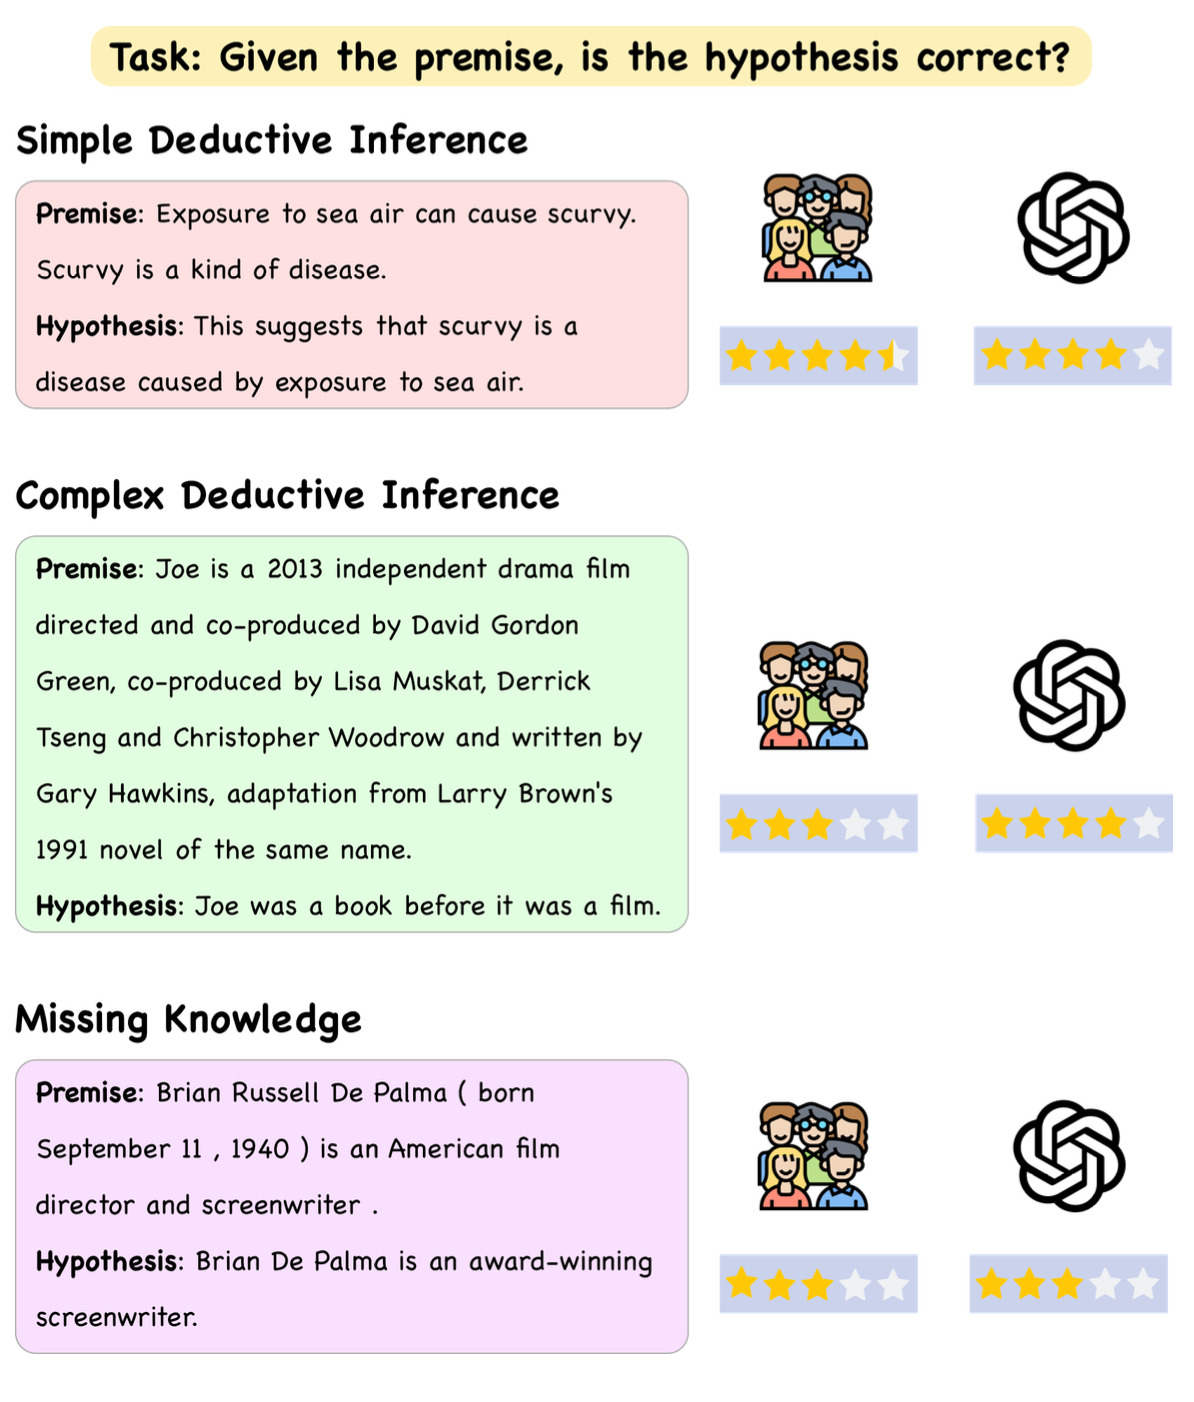
\includegraphics[width=0.6\textwidth]{res/rel-human-llm-inference}
    \end{minipage}
    \caption{Distinctions between human and LLM Inferences. The entailment prediction performance of humans and LLMs are depicted by a 5-star rating scale~\cite{sanyal2024machinesbettercomplexreasoning}.}
    \label{fig:distinguishing-human-llm-inferences}
\end{figure}

Interestingly, both perform comparably in situations requiring inference of missing knowledge.
One of the paper's key contributions is the fine-tuning of the Flan-T5~\cite{https://doi.org/10.48550/arxiv.2210.11416} model, which outperforms GPT-3.5 and performs at a comparable level to GPT-4, thus providing a robust, open-source solution for entailment verification tasks.
In contrast, the proposed approach to factulizing the knowledge graph using \ac{RAG} emphasizes the integration of external knowledge retrieval to ground factual assertions, which is critical for generating verifiable, accurate knowledge graphs.
While Sanyal et al. focus on the entailment between premises and hypotheses in textual inference, my work extends this by incorporating external evidence to ensure not just consistency but also factual correctness.

In comparison, the entailment verification tasks handled by Sanyal et al. emphasize reasoning within the constraints of the given context, whereas my \ac{RAG}-based approach highlights the necessity of retrieval from large external datasets to mitigate hallucinations and improve the factual grounding of generated content.
Both approaches deal with inference verification but diverge in their method of contextualizing and validating knowledge, with mine incorporating real-time retrieval for fact-checking.

This distinction is significant in terms of application: while their fine-tuned Flan-T5 model achieves high accuracy in entailment tasks, it remains bound to the contextual limits of its training data.
My work, by integrating retrieval, potentially overcomes this limitation by dynamically accessing external data, thus offering a complementary perspective to entailment verification focused on enhancing factuality.

\section{Claim Verification in the Age of Large Language Models}\label{sec:claim-verification-in-the-age-of-large-language-models}
Dmonte et al.~\cite{dmonte2024claimverificationagelarge} provide a comprehensive survey of \ac{LLM}-based approaches to claim verification, highlighting the shift from traditional \ac{NLP} methods to more sophisticated LLM-driven techniques.
The typical LLM-based claim verification pipeline, as described by Dmonte et al., consists of several key components:
\begin{enumerate}
    \item \textbf{Evidence Retrieval:} Utilizing techniques like \ac{RAG} to fetch relevant information from external sources.
    \item \textbf{Prompt Creation:} Developing effective prompting strategies to guide LLMs in processing claims and evidence.
    \item \textbf{Transfer Learning:} Employing fine-tuning and in-context learning to adapt LLMs to the specific task of claim verification.
    \item \textbf{LLM Generation:} Using LLMs to generate veracity labels, supporting evidence, and explanations.
\end{enumerate}

This pipeline represents a departure from traditional fact-checking approaches, leveraging the power of \ac{LLMs} to improve accuracy and provide more nuanced assessments of claim veracity.
Based on survey, several studies have demonstrated the effectiveness of LLM-based approaches in claim verification:
\begin{itemize}
    \item Zhang and Gao~\cite{zhang2023llmbasedfactverificationnews} introduced the Hierarchical Step-by-Step (HiSS) prompting method, which directs LLMs to separate a claim into several sub-claims and then verify each via multiple questions-answering steps progressively, improving performance on complex news claim verification tasks.
    \item Lee et al.~\cite{lee2023factualityenhancedlanguagemodels} developed FactualityPrompts, a framework for assessing the factual accuracy of LLM-generated content.
\end{itemize}

These studies consistently show that LLM-based methods outperform traditional NLP approaches in terms of accuracy, flexibility, and the ability to handle complex claims.

\begin{figure}[ht!]
    \centering
    \begin{minipage}[b]{\textwidth}
        \centering
        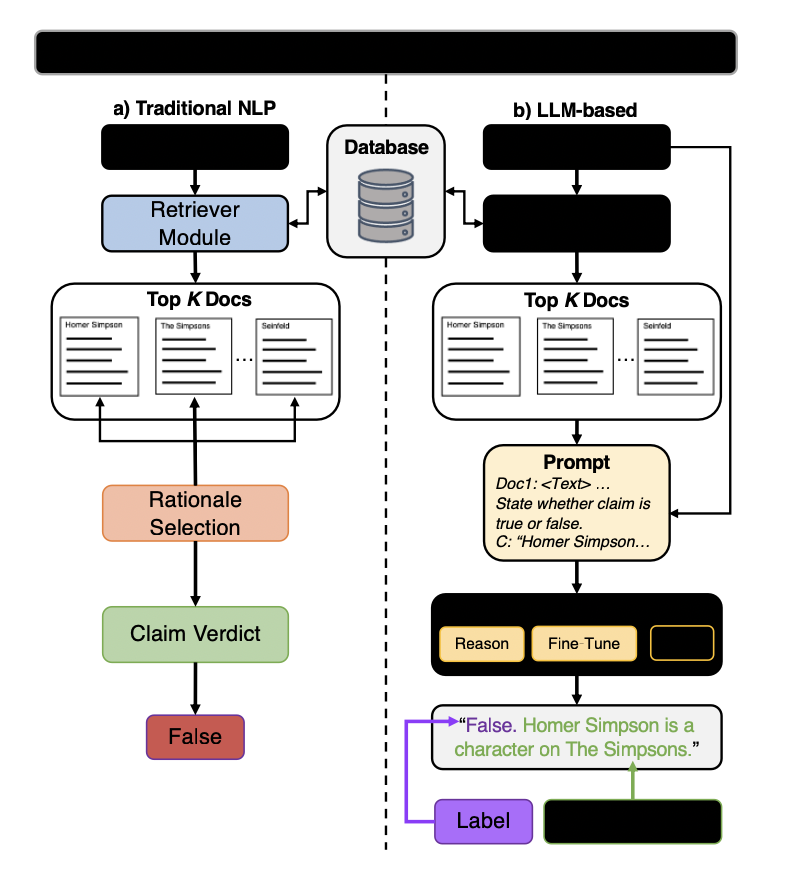
\includegraphics[width=0.6\textwidth]{res/rel-claim-verification}
    \end{minipage}
    \caption{Comparison of claim verification systems between NLP-based (traditional) and LLM-based for claim veracity.~\cite{dmonte2024claimverificationagelarge}.}
    \label{fig:claim-verification-llm}
\end{figure}

Our approach shares similarities with the LLM-based pipeline described by Dmonte et al., particularly in the use of retrieval-augmented generation and the integration of multiple LLMs. However, our method differs in several key aspects:
\begin{enumerate}
    \item \textbf{Multi-Query Retrieval:} We employ a multi-query strategy for evidence retrieval, potentially improving the coverage and relevance of supporting information.
    \item \textbf{Iterative Refinement:} Our system incorporates an iterative process for refining retrieved evidence and generated responses, which is not explicitly mentioned in most LLM-based approaches surveyed.
    \item \textbf{Limited Explanation:} While many LLM approaches provide explanations, our method places a stronger emphasis on generating binary (pass/fail) labels for claims to reduce the costs of using LLMs.
    \item \textbf{Diverse LLM Model:} We use multiple LLMs with diverse architectures to provide more reliable verification result.
\end{enumerate}

These distinctions position our work as a novel contribution to the field, building upon the foundations of LLM-based claim verification while introducing innovative techniques to enhance performance and interpretability.

Despite the promising results of LLM-based claim verification, several challenges remain.
Dmonte et al. highlight issues such as handling irrelevant context, resolving knowledge conflicts, and expanding to multilingual settings. Our approach attempts to address some of these challenges, particularly in the areas of context relevance and explainability. However, there is still significant room for improvement in creating more robust, reliable, and universally applicable claim verification systems.

\section{Retrieval-Augmented Fact Verification by Synthesizing Contrastive Arguments}\label{sec:retrieval-augmented-fact-verification}
The paper Retrieval-Augmented Fact Verification by Synthesizing Contrastive Arguments~\cite{yue2024retrievalaugmentedfactverification} explores a method for improving fact verification in knowledge graphs using RAG.
The proposed framework combines retrieval of external information and the generation of contrastive arguments-claims supported by retrieved evidence, but also those that provide counterpoints.
This dual synthesis provides a richer and more nuanced verification process, allowing the system to handle conflicting evidence more effectively.
The core contribution of the work lies in the creation of contrastive arguments, a strategy designed to reduce errors in fact verification systems, especially when LLMs may hallucinate or generate incomplete reasoning.

The authors leverage a multi-stage pipeline where external documents are retrieved to support or refute a given claim.
Each retrieved piece of evidence is evaluated using a neural network model that ranks the evidence based on its relevance to the claim.
By synthesizing contrastive arguments, the system generates explanations for both supporting and refuting the claim, which helps improve the transparency and trustworthiness of the model's decisions.

\begin{figure}[ht!]
    \centering
    \begin{minipage}[b]{\textwidth}
        \centering
        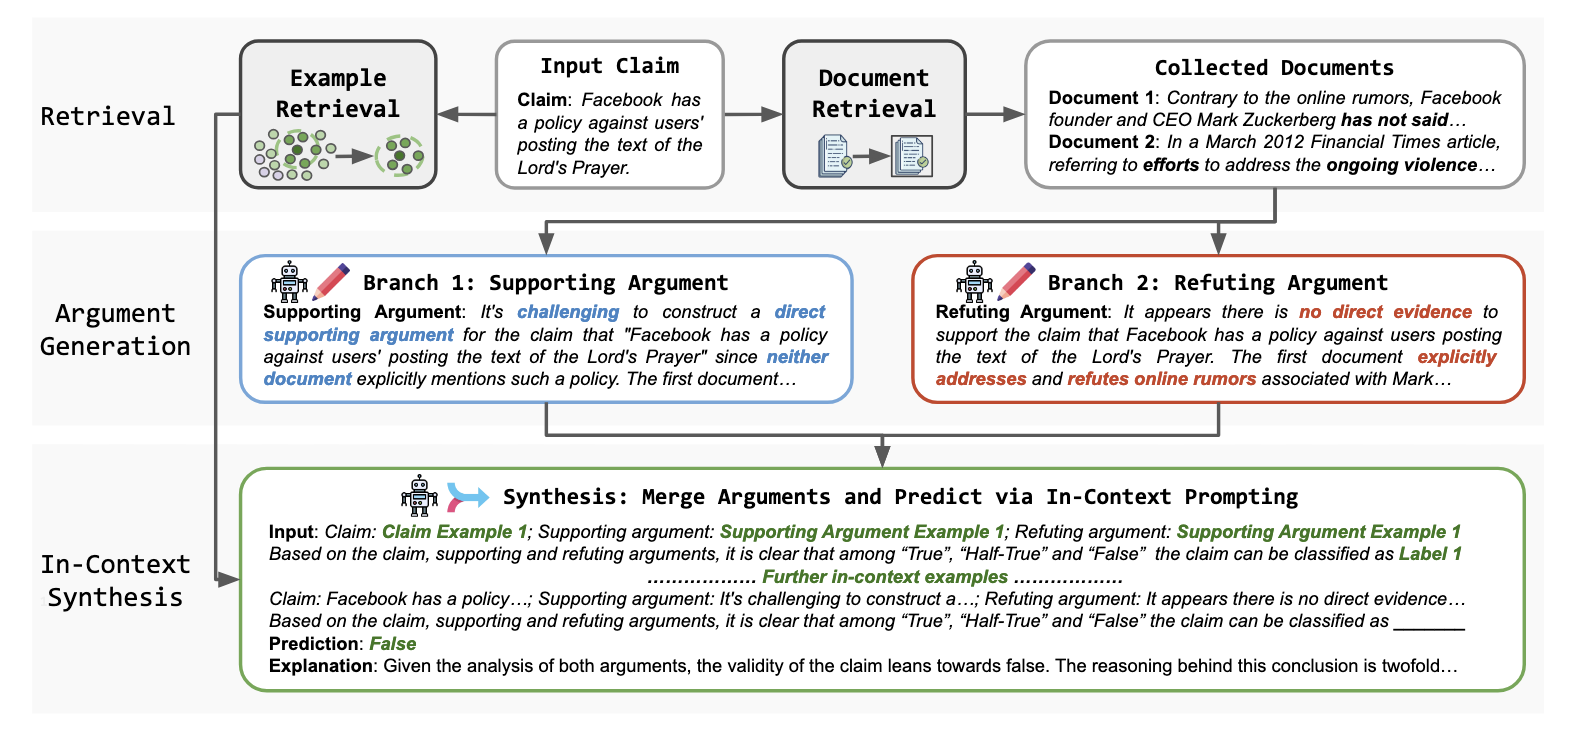
\includegraphics[width=\textwidth]{res/rel-rafts}
        \caption{The proposed RAFTS~\cite{yue2024retrievalaugmentedfactverification}, which performs few-shot fact verification by incorporating informative in-context demonstrations and contrastive arguments with nuanced information derived from the retrieved documents}
        \label{fig:rel-rafts}
    \end{minipage}
\end{figure}

In terms of results, the framework shows improvement over traditional fact verification pipelines, particularly in handling ambiguous or conflicting information.
The contrastive arguments allow for better handling of cases where facts are not binary but exist in a more complex, nuanced state.
The system's ability to generate arguments for both sides of a claim increases its robustness and provides a more reliable fact verification tool.

The described approach and my work on fact verification in knowledge graphs using RAG share a common goal: improving the factual accuracy of information through the integration of external knowledge retrieval.
However, there are key differences in the methodologies used.
The contrastive argument synthesis introduced by the authors focuses heavily on generating both supporting and opposing arguments for claims, which provides a more holistic perspective in scenarios where evidence is mixed.
In contrast, my approach emphasizes majority voting among multiple models and a multi-query strategy to retrieve a broader range of external evidence, aiming to reduce the incidence of hallucinations in LLM outputs.

While both approaches use retrieval to mitigate the limitations of LLMs, my work incorporates adaptive dispute resolution techniques and focuses on synthesizing outputs from multiple LLMs rather than generating contrastive arguments.
This means that my approach leans more towards optimizing model diversity and utilizing the best consensus from several LLMs to ensure factual accuracy, rather than explicitly generating opposing arguments for each claim.

\section{RAGAR: RAG-Augmented Reasoning for Political Fact-Checking using Multimodal LLMs}\label{sec:agar-rag-augmented-reasoning}
The study titled RAGAR: RAG-Augmented Reasoning for Political Fact-Checking using Multimodal LLMs~\cite{khaliq2024ragarfalsehoodradarragaugmented} introduces a novel approach to political fact-checking by leveraging RAG with multimodal LLMs.
This work focuses on enhancing fact verification in the politically sensitive domain, where disinformation can have far-reaching consequences.
The authors integrate various modalities text, images, and other media sources into a unified fact-checking pipeline powered by LLMs, particularly emphasizing RAG’s ability to retrieve and synthesize external evidence to validate or refute claims.

\begin{figure}[ht!]
    \centering
    \begin{minipage}[b]{\textwidth}
        \centering
        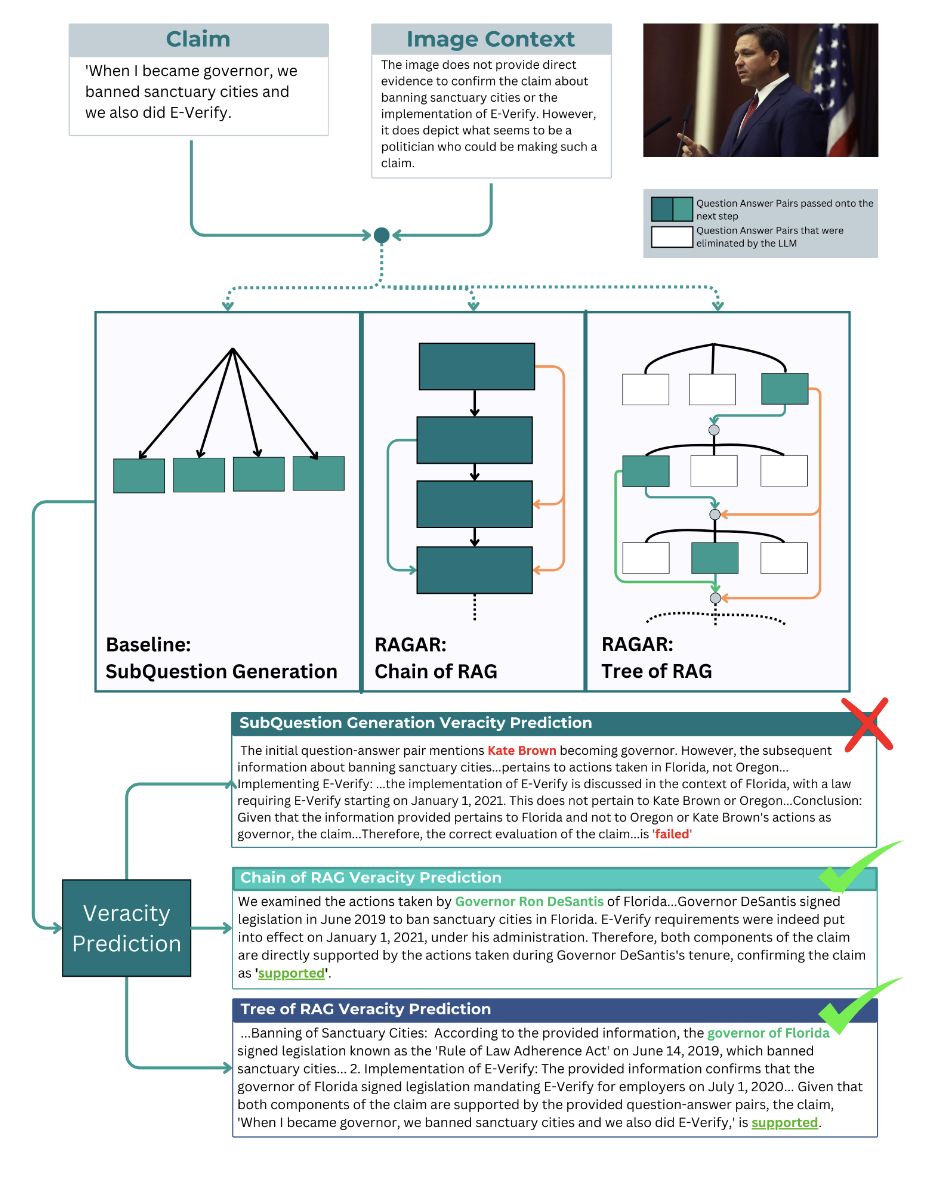
\includegraphics[width=0.6\textwidth]{res/rel-ragar}
    \end{minipage}
    \caption{An overview of the fact-checking pipeline contrasting the baseline Sub-Question Generation approach from the Chain of RAG and Tree of RAG approach followed by veracity prediction and explanation.}
    \label{fig:rel-ragar}
\end{figure}

The central innovation of RAGAR lies in its multimodal reasoning capabilities, which allow the model to handle political claims that involve not only textual content but also visual data, such as images or charts.
By extending RAG to this multimodal context, the system improves its ability to assess the veracity of claims in real-time, leveraging external resources such as political databases and live web content.
Furthermore, the use of contrastive learning helps the system generate both supporting and opposing arguments for each claim, providing a more balanced and comprehensive fact-checking process.

Results from the paper show significant improvements in fact-checking accuracy, particularly for politically charged claims that are often more nuanced or context-dependent.
RAGAR's ability to synthesize multimodal evidence into a coherent verification report highlights its potential for real-world applications, especially in environments where disinformation spreads quickly, such as social media platforms.

RAGAR focuses on political fact-checking using multimodal data, whereas my work targets the factualization of knowledge graphs with a primary focus on textual information.
In contrast to RAGAR’s multimodal pipeline, my system emphasizes multi-query strategies and document chunking techniques to retrieve highly relevant textual evidence for verification.
    \chapter{Pipeline}\label{ch:pipeline}
This chapter presents a detailed examination of a multi-stage NLP pipeline designed to enhance information retrieval and question answering capabilities.
The pipeline integrates various cutting-edge technologies and methodologies, creating a synergistic system that pushes the boundaries of what is possible in automated information processing and response generation.
However, the challenges of accurately interpreting user queries, retrieving relevant information from vast datasets, and generating coherent and contextually appropriate responses remain significant.
This pipeline addresses these challenges through a carefully orchestrated series of processes, each designed to refine and enhance the quality of information flow from input to output.

At its core, the pipeline leverages a knowledge graph dataset, serving as the foundational repository of interconnected information.
This graph structure allows for the representation of complex relationships between entities, facilitating more nuanced understanding and retrieval of information.
The pipeline then employs a series of sophisticated mechanisms, including query generation, cross-encoding for relevance assessment, and multi-tiered information retrieval strategies, to navigate this knowledge landscape effectively.

One of the key innovations in this pipeline is its approach to context processing and information synthesis.
By breaking down retrieved information into manageable chunks and employing advanced embedding techniques, the system can perform more granular and accurate analyses of textual data.
This granularity, combined with the implementation of multiple LLMs working in concert, allows for a more robust and nuanced interpretation of complex queries and generation of comprehensive responses.

The integration of external information sources, notably through the incorporation of Google Search capabilities, further enhances the pipeline's ability to access and process up-to-date and diverse information.
This hybrid approach, combining structured knowledge graphs with dynamic web-based information retrieval, positions the pipeline at the forefront of adaptive and responsive AI systems.

Critical to the pipeline's effectiveness is its sophisticated decision-making architecture.
Employing strategies such as majority voting among multiple models and the implementation of a final judge for conflict resolution, the system strives to achieve a balance between diverse perspectives and the need for coherent, unified outputs.
This approach not only enhances the accuracy and reliability of the generated responses but also provides a framework for managing the inherent uncertainties and potential biases in AI-driven decision-making processes.

As we delve deeper into each component of this pipeline, it is crucial to maintain a critical perspective on both its capabilities and limitations.
While the system represents a significant advancement in NLP and information retrieval technologies, it also raises important questions about the ethical implications of AI-driven information processing, the potential for bias in knowledge representation and model training, and the broader societal impacts of increasingly sophisticated question-answering systems.

This chapter aims to provide a comprehensive analysis of each stage of the pipeline, examining not only the technical aspects of its implementation but also the theoretical underpinnings and practical implications of its design choices.
By understanding the intricacies of this system, we can gain valuable insights into the current state of NLP technologies and the potential future directions for research and development in this rapidly advancing field.
As we proceed, we will explore each component in detail, starting with the foundational knowledge graph dataset and progressing through the various stages of query processing, information retrieval, context analysis, and response generation.
This exploration will shed light on the complex interplay between different AI technologies and methodologies, offering a holistic view of how modern NLP systems can be architected to tackle some of the most challenging problems in information processing and human-computer interaction.


\section{Knowledge Graph Dataset}\label{sec:knowledge-graph-dataset}
The foundation of our multi-stage RAG pipeline is the Knowledge Graph Dataset, which acts as the primary source of factual information for the ensuing processing stages.
This section clarifies the attributes and aims of the knowledge graph and its use in our pipeline.

\subsection{Definition and Purpose}\label{subsec:definition-and-purpose}
In the form of a graph, a knowledge graph is an ordered way to show information that models real-world things and how they relate to each other.
The Knowledge Graph Dataset is a huge collection of facts, ideas, and connections that are all linked together in our process.
Its main job is to give a lot of background information so that complicated queries can be understood and processed.

The implementation of a knowledge graph fulfills multiple essential functions:
\begin{itemize}
    \item \textbf{Semantic Representation:} Unlike traditional relational databases, knowledge graphs capture semantic relationships between entities, allowing for more nuanced and context-aware information retrieval.
    \item \textbf{Inferential Capabilities:} The interconnected nature of the graph enables the system to make inferences and connections that may not be explicitly stated, enhancing the depth and breadth of responses.
    \item \textbf{Scalability:} Knowledge graphs can efficiently handle large volumes of heterogeneous data, making them ideal for systems that need to process diverse types of information.
    \item \textbf{Flexibility:} The graph structure allows for easy updates and expansions, ensuring that the knowledge base can evolve with new information and changing requirements.
\end{itemize}

\subsection{Structure and Components}\label{subsec:structure-and-components}
The Knowledge Graph Dataset in our pipeline is composed of several key components:
\begin{itemize}
    \item \textbf{Nodes:} Representing entities or concepts, nodes are the fundamental units of information in the graph. Each node typically corresponds to a distinct piece of knowledge, such as a person, place, event, or abstract concept.
    \item \textbf{Edges:} These are the connections between nodes, representing relationships or interactions. Edges are often directional and labeled to indicate the nature of the relationship (e.g., "is\_a", "part\_of", "created\_by").
    \item \textbf{Properties:} Nodes and edges can have associated properties or attributes that provide additional details or metadata about the entity or relationship.
\end{itemize}

\subsection{Role in the Overall Pipeline}\label{subsec:role-in-the-overall-pipeline}
As illustrated in the pipeline diagram, the Knowledge Graph Dataset is the thing that we want to verify the correctness of it.
The pipeline uses the knowledge graph to generate queries, retrieve relevant information, and synthesize responses to find the correctness of the knowledge graph.

\section{Query Generation and Processing}\label{sec:query-generation-and-processing}
The Query Generation and Processing step, following to the basic Knowledge Graph Dataset, is a pivotal point in our pipeline, wherein user inputs are converted into structured queries suitable for efficient processing by later components.
This section clarifies the techniques and methodologies utilized in this critical phase for subsequent actions in the information retrieval process.

\subsection{Human-Understandable Text Generation}\label{subsec:human-understandable-text-generation}
In the first step of the pipeline, we use a LLM (ie. LLama3~\cite{dubey2024llama3herdmodels}, Gemma2~\cite{gemmateam2024gemma2improvingopen}) to easily generate human-readable text by submitting prompts.
This approach bridges the gap between representing raw data and conveying it in natural language, making the information more accessible and understandable.
For additional information, consult the prompt template in Appendix~\ref{sec:prompt-templates:human-understandable} to observe the sentence generation process.

Key aspects of this process include:
\begin{itemize}
    \item \textbf{Contextual Awareness:} Integrating relevant context from the Knowledge Graph to guarantee that the output content is relevant and useful.
    \item \textbf{Adaptability:} Customizing the generated text to accommodate various complexity levels, catering to diverse user needs and query types.
    \item \textbf{Semantic Enrichment:} Enhancing the generated text with semantic annotations to facilitate more accurate downstream processing.
\end{itemize}

Be aware that certain knowledge graph datasets are human-readable, whereas others are not; for instance, the FactBench~\cite{GERBER201585} dataset may be easily comprehended by concatenating the subject, predicate, and object of each triple.
% TODO: DBpedia refrence needed to be added
\begin{table}[h!]
    \noindent
    \resizebox{\textwidth}{!}{
        \begin{tabular}{p{3cm} p{3cm} p{3cm} c c p{3cm}}
            \toprule
            \multicolumn{3}{c}{\textbf{Knowledge Graph}} & \multirow{2}{*}{\textbf{Source}} & \multirow{2}{*}{\textbf{Is Generated ?}} & \multirow{2}{*}{\textbf{Final Text}} \\
            \cmidrule(lr){1-3} \
            Subject & Predicate & Object & & & \\
            \midrule
            \textit{Albert Einstein} & \textit{Birth Place} & \textit{Ulm, Germany} & FactBench~\cite{GERBER201585} & \ding{55} & \textit{Albert Einstein birth place Ulm, Germany} \\
            \textit{Chris Benoit} & \textit{deathPlace} & \textit{Fayetteville, Georgia} & FactBench~\cite{GERBER201585} & \ding{55} & \textit{Chris Benoit death place Fayetteville, Georgia} \\
            \hdashline
            \textit{Alexander\_III \_of\_Russia} & \textit{isMarriedTo} &\textit{Maria\_Feodorovna \_\_Dagmar\_of\_Denmark\_} & YAGO~\cite{suchanek2024yago45largeclean} & \ding{51} & \textit{Alexander III of Russia is married to Maria Feodorovna, also known as Dagmar of Denmark.} \\
            \hdashline
            \textit{Shock\_to\_the \_System \_(Gemma\_Hayes \_song)} & \textit{length} & \textit{221.0} & DBpedia & \ding{51} & \textit{The length of Shock to the System (Gemma Hayes song) is 221.0.} \\
            \textit{Paora\_Winitana} & \textit{years} & \textit{2011} & DBpedia & \ding{51} & \textit{Paora Winitana was active in 2011.} \\
            \bottomrule
        \end{tabular}}\caption{Generation of Human-Understandable Text}
    \label{tab:Text-Generation}
\end{table}

\subsection{Question Formulation Techniques}\label{subsec:question-formulation-techniques}
A cornerstone of our pipeline is its ability to generate 10 questions about the input sentence, as illustrated in the diagram.

This multi-question approach serves several purposes:
\begin{itemize}
    \item \textbf{Comprehensive Coverage:} By generating multiple questions, the system ensures a thorough exploration of the input's various aspects and potential interpretations.
    \item \textbf{Disambiguation:} Multiple questions help in clarifying ambiguities that may be present in the original input.
    \item \textbf{Context Expansion:} Each generated question potentially introduces new contextual elements, broadening the scope of the subsequent information retrieval process.
    \item \textbf{Robustness:} The diversity of questions increases the likelihood of capturing the user's true intent, even if the original input is vague or imprecise.
\end{itemize}

Implementation of this technique likely involves:
Using \ac{LLMs} to generate 10 questions about the input sentence, leveraging the models' language understanding capabilities to ensure the questions are relevant and contextually appropriate.
The prompt template used to guide the question generation process reported in Appendix~\ref{sec:prompt-templates:10-question}.

\subsection{Cross-Encoder for Query Relevance Scoring}\label{subsec:cross-encoder-for-query-relevance-scoring}
The Cross-Encoder component is essential for evaluating the relevance of the generated questions.
As indicated in the Figure~\ref{fig:cross-encoder-articture}, this module takes multiple inputs and produces relevance scores for each question.

\begin{figure}[ht!]
    \centering
    \begin{minipage}[b]{\textwidth}
        \centering
        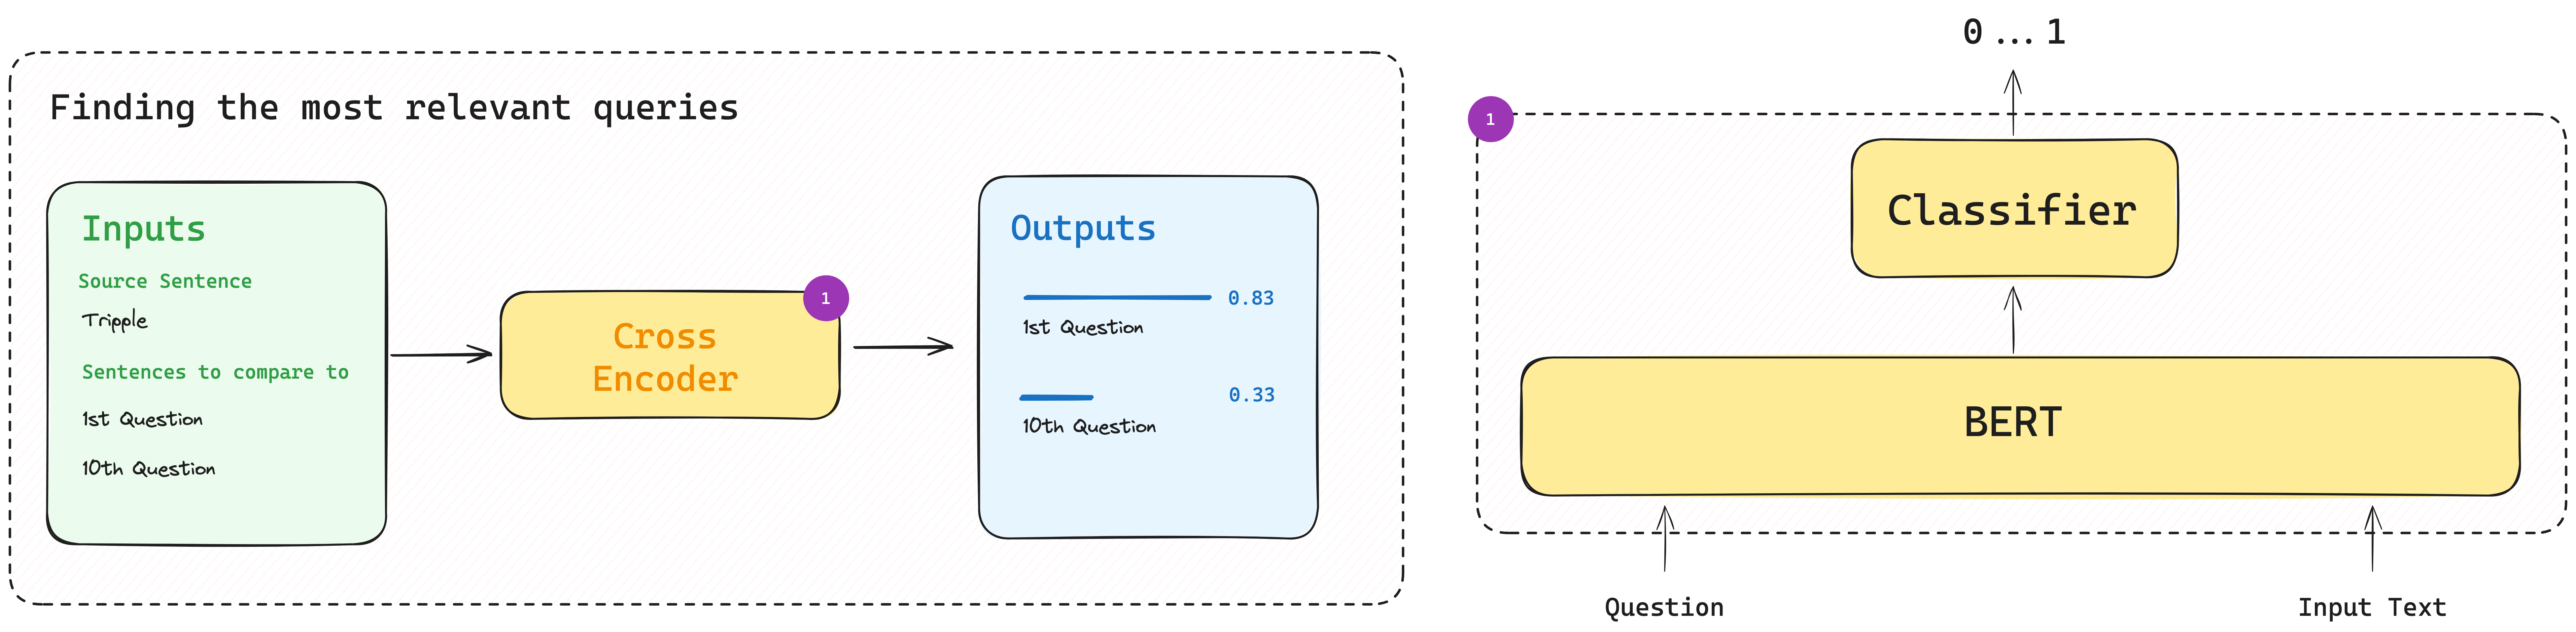
\includegraphics[width=\textwidth]{res/Cross-Encoder}
        \caption{Cross-Encoder Architecture}
        \label{fig:cross-encoder-articture}
    \end{minipage}
\end{figure}

Key features of the Cross-Encoder include:

\begin{itemize}
    \item Input Processing
    \begin{itemize}
        \item Source Sentence: The original input text.
        \item Sentences to Compare: Likely the 10 generated questions.
    \end{itemize}
    \item Scoring Mechanism: The Cross-Encoder assigns numerical scores (e.g., 0.83 as shown in the figure~\ref{fig:cross-encoder-articture}) to each question, indicating its relevance to the source sentence.
    \item Comparative Analysis: By processing all inputs simultaneously, the Cross-Encoder can perform nuanced comparisons between the original input and each generated question, as well as among the questions themselves.
\end{itemize}

In this case we use the \textit{jinaai/jina-reranker-v1-turbo-en}\footnote{\url{https://huggingface.co/jinaai/jina-reranker-v1-turbo-en}} model from the Hugging Face Transformers library.
This model is designed for blazing-fast re-ranking while maintaining competitive performance.
It leverages the power of JinaBERT~\cite{günther2024jinaembeddings28192token} model as its foundation.
The model employs a process known as knowledge distillation to attain exceptional speed and efficiency, making it the optimal selection for our pipeline.

\begin{figure}[ht!]
    \centering
    \begin{minipage}[b]{\textwidth}
        \centering
        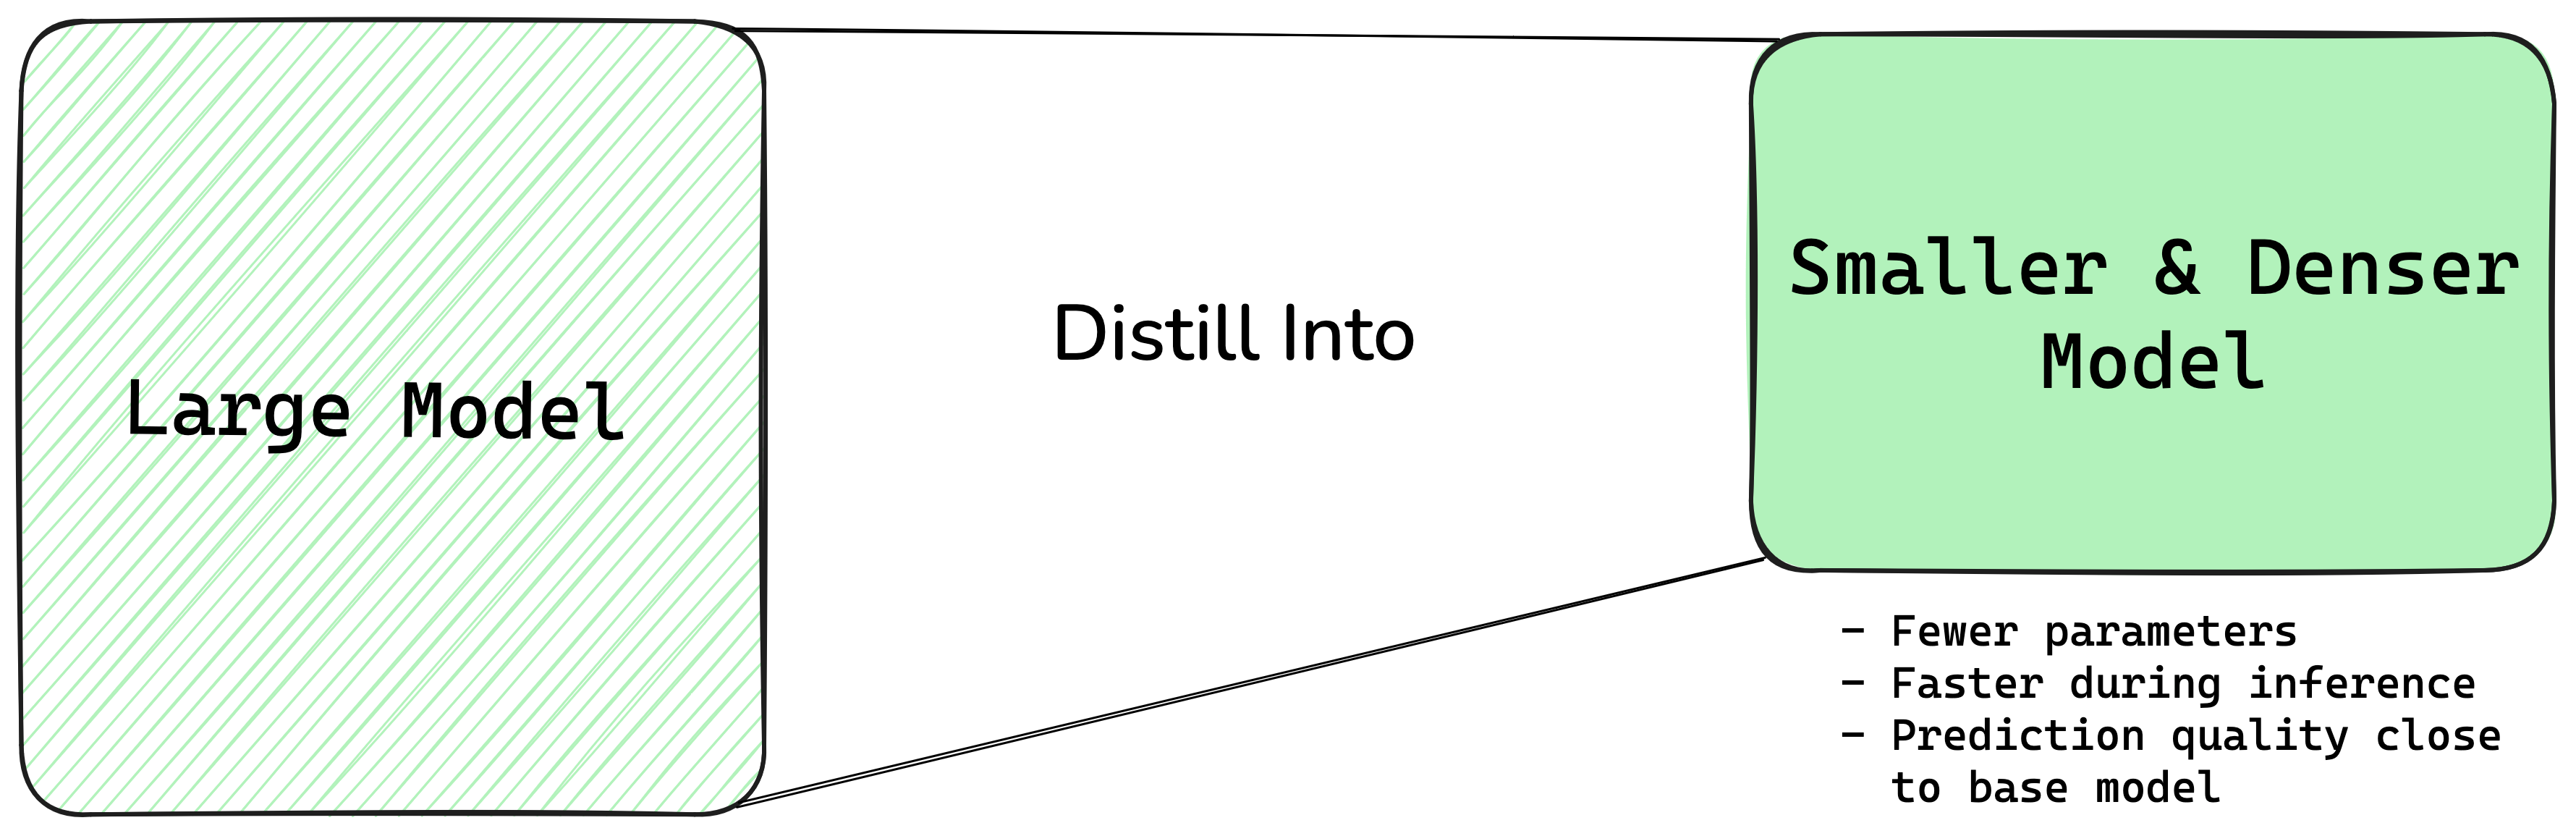
\includegraphics[width=0.7\textwidth]{res/knowledge-distill}
        \caption{Knowledge Distillation Process}
        \label{fig:knowledge-distill}
    \end{minipage}
\end{figure}

\begin{table}[h!]
    \noindent
    \resizebox{\textwidth}{!}{
        \begin{tabular}{llc}
            \toprule
            \textbf{Input} & \textbf{Question} & \textbf{score} \\
            \midrule
            \multirow{10}{*}{\shortstack[l]{\textit{Frédéric Passy} \\ \textit{award} \\ \textit{Nobel Peace Prize}}} & Who was awarded the Nobel Peace Prize? & 0.7458 \\
            & What award did Frédéric Passy receive? & 0.7121 \\
            & Is Frédéric Passy a Nobel laureate? & 0.8706 \\
            & In what category was the Nobel Peace Prize awarded to Frédéric Passy? & \textbf{0.9491} \\
            & Who is known for receiving the Nobel Peace Prize? & 0.5823 \\
            & What is the name of the award received by Frédéric Passy? & 0.6318 \\
            & Is Frédéric Passy a recipient of the Nobel Prize in any field? & 0.7652 \\
            & Who was recognized for his work towards peace? & 0.1457 \\
            & What is the significance of the award given to Frédéric Passy? & 0.6036 \\
            & Is there a Nobel laureate with the name Frédéric Passy? & 0.8505 \\
            \bottomrule
        \end{tabular}}\caption{Question Generation and Scoring Procedure}
    \label{tab:Question scoring}
\end{table}

\subsection{Relevance Threshold and Sorting}\label{subsec:relevance-threshold-and-sorting}
Following the Cross-Encoder's scoring, the pipeline implements a crucial decision point:
\begin{itemize}
    \item \textbf{Sorting:} Questions are sorted based on their relevance scores, establishing a priority order for further processing.
    \item \textbf{Threshold Evaluation:} The system checks if the top question's score exceeds an upper threshold. This step ensures that only sufficiently relevant questions proceed further in the pipeline.
    \item \textbf{Feedback Loop:} If the threshold is not met, the process must loop back to generate new questions to adjust the existing ones, maintaining the quality of queries entering subsequent stages.
\end{itemize}

\section{Information Retrieval Mechanisms}\label{sec:information-retrieval-mechanisms}
The Information Retrieval Mechanisms are an essential element of our pipeline, connecting query processing and content synthesis.
This phase is tasked with gathering relevant data from internal and external sources, thereby establishing a comprehensive data repository for further analysis and response formulation.
The mechanisms employed in this phase are designed to ensure breadth, depth, and relevance in the retrieved information.

\subsection{Google Search Integration}\label{subsec:google-search-integration}
A key feature of our information retrieval process is the integration of Google Search capabilities, as prominently displayed in the pipeline diagram.
This integration serves to expand the information horizon beyond the confines of our internal Knowledge Graph Dataset.
Key aspects of this integration include:

\begin{itemize}
    \item \textbf{Query Submission:} The system submits the N top questions (where N is a predefined number) along with the main question to Google Search. This approach ensures a multi-faceted search that captures various aspects of the original query.
    \item \textbf{Result Fetching:} As indicated in the diagram, the system retrieves the top 100 search results. This number strikes a balance between comprehensiveness and computational efficiency.
    \item \textbf{Dynamic Information Access:} By leveraging Google Search, the system gains access to up-to-date information, complementing the more static nature of the internal Knowledge Graph.
    \item \textbf{Diverse Source Types:} Google Search results typically include a variety of source types (e.g., websites, news articles, academic papers), enriching the diversity of the retrieved information.
\end{itemize}

\begin{figure}[ht!]
    \centering
    \begin{minipage}[b]{\textwidth}
        \centering
        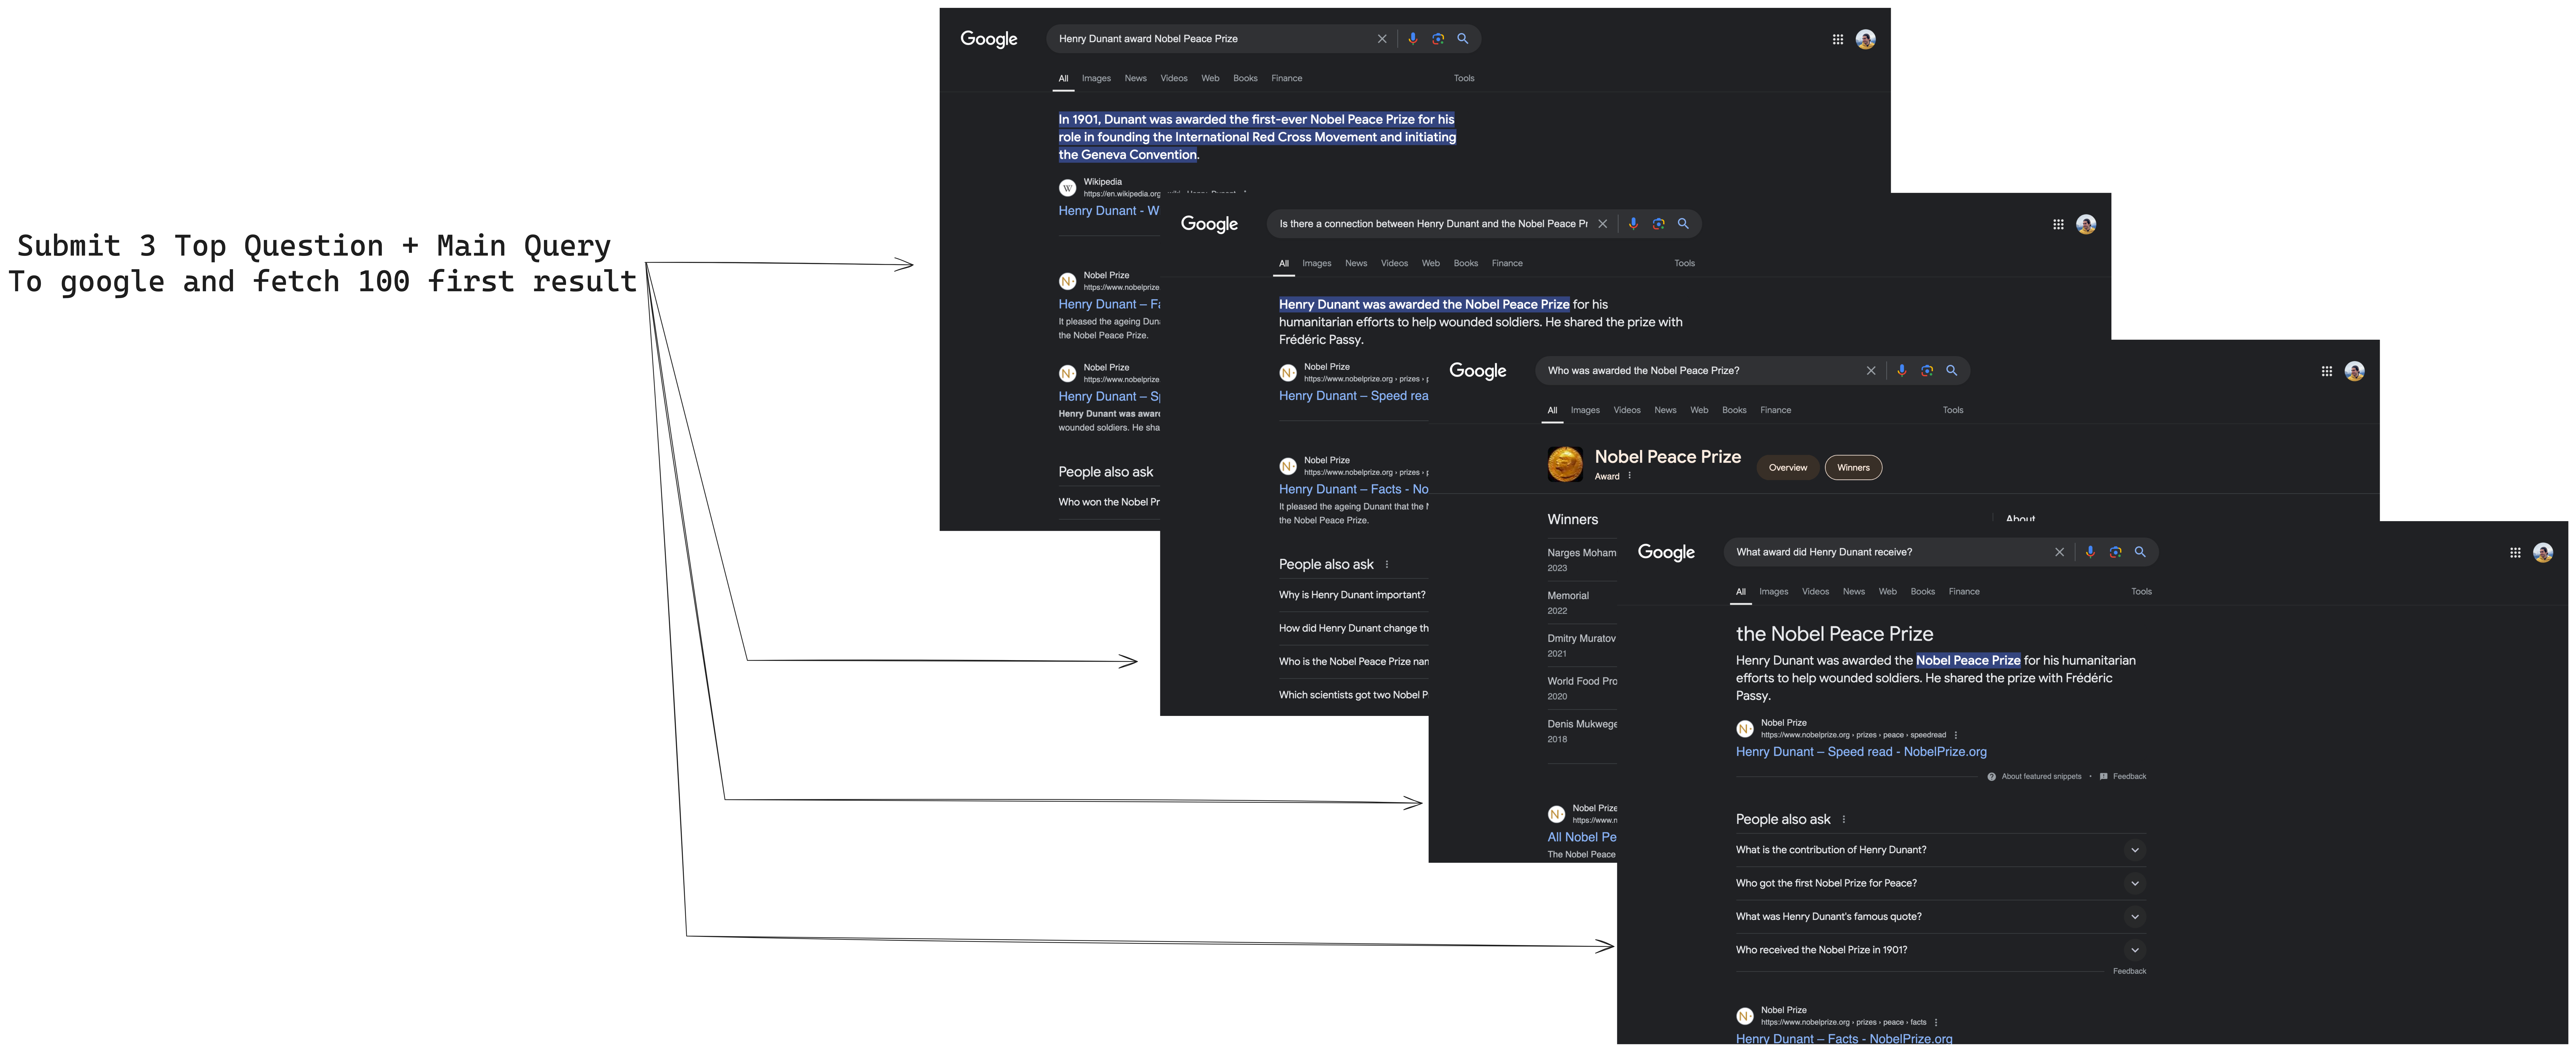
\includegraphics[width=\textwidth]{res/Google-Search-Result}
        \caption{Fetching the results from Google Search}
        \label{fig:google-search-result}
    \end{minipage}
\end{figure}

Implementation considerations:
\begin{itemize}
    \item The system may employ proxies or other mechanisms to manage rate limits and ensure uninterrupted access to search results.
    \item The search query may be customized based on the specific requirements of the pipeline, such as language restrictions, geolocation preferences, or result quantity. parameters are lr, hl, gl, and num.
\end{itemize}

Take note that the code base is generic, and it means that you can use any search engine, not only Google Search.

\subsection{Process and Extract Links}\label{subsec:process-and-extract-links}
Following the retrieval of search results, the pipeline incorporates a crucial step of processing and extracting links from the gathered information.
This process likely involves:
\begin{itemize}
    \item \textbf{Parsing \ac{HTML} Content:} Extracting relevant textual information from the retrieved web pages.
    \item \textbf{Link Analysis:} Identifying and cataloging hyperlinks within the content, potentially uncovering additional relevant sources.
\end{itemize}

After Parsing the HTML content of the Google Search results, the system use HTML selectors to extract the links from the search results.
In this case we also extract the title, url, description, price, date, duration, missing, rating, availability, and extra details from the search results.
Some of the information mentioned above may not be available as it depends on the search results.

Then there is a need to crawl the extracted links to get the content of the page, for doing this we use the Python library called \textit{GRequests}\footnote{\url{https://pypi.org/project/grequests/}}.
\textit{GRequests} is a Python library that combines the power of gevent for asynchronous I/O with the simplicity of the Requests library for HTTP operations. It allows developers to perform concurrent HTTP requests easily, significantly speeding up operations that involve multiple API calls or web scraping tasks.

\begin{lstlisting}[language=Python, caption=Crawling the Extracted URLs, label=lst:crawling-urls]
import os
import grequests
from fake_useragent import UserAgent

ua = UserAgent(
    os=['windows'],
    browsers=["chrome", "edge", "firefox"],
    platforms=["pc"]
)

urls = [...List of Extracted URLs...]

rs = [
    grequests.get(u['url'],
    timeout=3, headers={"User-Agent": ua.random}) for u in urls
]
for index, response in grequests.imap_enumerated(rs, size=50):
    if response is None or response.status_code != 200:
        continue
    # Process the response content ...
\end{lstlisting}

There are several faults in the mentioned approach~\ref{lst:crawling-urls} that need to be addressed:
\begin{itemize}
    \item \textbf{Site generated with javascript:} The provided approach does not handle sites that are generated with JavaScript and require dynamic rendering.
    \item \textbf{Protection against scraping:} Sites may have protection mechanisms against scraping, such as CAPTCHAs or IP blocking or behind spam protection services.
    \item \textbf{Login required:} Some sites require login credentials to access the content.
\end{itemize}

We can use the \textit{Selenium}\footnote{\url{https://www.selenium.dev/}} library to handle the first issue, and for the second and third issues, we can use the \textit{Scrapy}\footnote{\url{https://scrapy.org/}} library, but we stick with the provided approach for simplicity and speed.

With the extracted content, the system can now proceed to the next stage of the pipeline, where the information is further processed and analyzed.
For extracting the content of the page, as our webpage are from vast sources, we need to use a robust and efficient library to extract the content of the page.
We use \textit{newspaper4k}\footnote{\url{https://newspaper4k.readthedocs.io/en/latest/}} library to extract the content of the page.
\textit{newspaper4k} is a Python library designed for extracting and parsing newspaper articles. It's an updated and improved version of the original newspaper3k library, offering enhanced functionality and compatibility with modern Python versions.

Key features of the \textit{newspaper4k} library include:
\begin{itemize}
    \item \textbf{Article Extraction:} Easily extract articles from news websites.
    \item \textbf{Multi-language Support:} Capable of processing articles in various languages.
    \item \textbf{Full-text Extraction:} Extracts the full text of articles, removing ads and extraneous content.
    \item \textbf{Keyword Extraction:} Automatically identifies key topics and keywords from articles.
    \item \textbf{Summary Generation:} Creates concise summaries of article content.
    \item \textbf{Metadata Parsing:} Extracts metadata such as authors, publication dates, and tags.
    \item \textbf{Image Extraction:} Identifies and extracts images associated with articles.
\end{itemize}

\begin{figure}[ht!]
    \centering
    \begin{minipage}[b]{\textwidth}
        \centering
        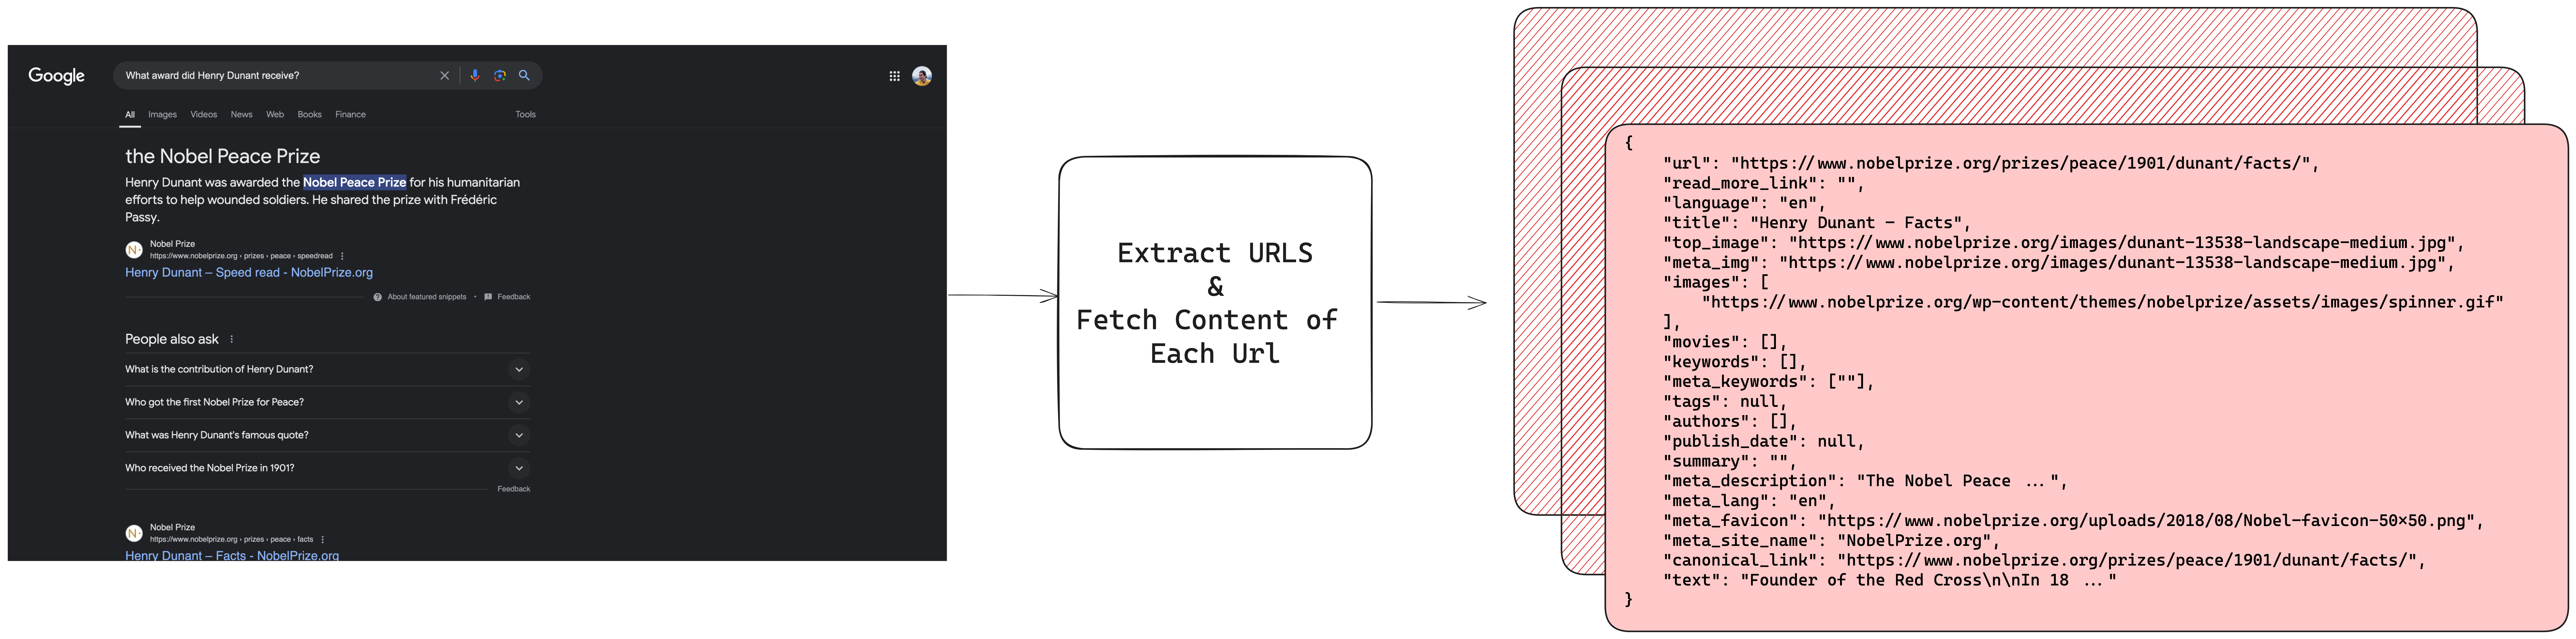
\includegraphics[width=\textwidth]{res/Google-Search-Result-Content}
        \caption{Extracted Content from the Crawled URLs using newspaper4k}
        \label{fig:google-search-result-content}
    \end{minipage}
\end{figure}

For our purpose, we only use the text content of the page.
\subsection{Data Pool Creation}\label{subsec:data-pool-creation}
The processed and extracted information culminates in the creation of a data pool, a centralized repository of relevant information that serves as the foundation for subsequent stages of the pipeline.

Key features of the data pool include:
\begin{itemize}
    \item \textbf{Structured Storage:} Organizing the retrieved information in a format that facilitates efficient querying and analysis.
    \item \textbf{Source Diversity:} Maintaining a balance between information from web searches and the internal Knowledge Graph.
    \item \textbf{Relevance Scoring:} Potentially implementing a scoring system to prioritize more relevant or authoritative pieces of information within the pool.
    \item \textbf{Deduplication:} Employing mechanisms to identify and merge duplicate or highly similar pieces of information to reduce redundancy.
\end{itemize}
\subsection{Data filtering}\label{subsec:data-filtering}
The data filtering process aims to refine our data pool by removing information from sources that are already part of creation of the Knowledge Graph.
This ensures the uniqueness and independence of our data, for example, when working with the FactBench dataset, we exclude data from the following sources: wikipedia.org, wikimedia.org, wikidata.org and other similar wiki-based platforms.

On the other hand, we just keep the top 10 relevant information for the pipeline using cross-encoders discussed in Section~\ref{subsec:cross-encoder-for-query-relevance-scoring}, this way we ensure about the quality of the data.
More details about the data filtering process methodology are provided in the section~\ref{sec:document-selction}.

Specifically:
\begin{itemize}
    \item We start with a larger pool of data.
    \item We identify sources that are already the source of the Knowledge Graph.
    \item We remove any data points that come from these identified sources.
\end{itemize}

\section{Embedding and Retrieval Tasks}\label{sec:embedding-and-retrieval-tasks}
An important step in our pipeline is the Embedding and Retrieval Tasks, which connect machine-interpretable vector representations to unprocessed textual input.
This component is essential for improving the efficiency and accuracy of information retrieval and subsequent processing stages.

This section emphasizes embedding for retrieval tasks, specifically for small information segments, as depicted in the pipeline diagram.

\subsection{Embedding Techniques for Smaller Chunks}\label{subsec:embedding-techniques-for-smaller-chunks}
The pipeline employs advanced embedding techniques to transform textual data into dense vector representations, facilitating more efficient and semantically aware retrieval processes.

Key aspects of this embedding process include:
\begin{itemize}
    \item \textbf{Granularity:} The focus on \"Smaller Chunks\" suggests a fine-grained approach to embedding, where text is broken down into manageable units. This granularity allows for more precise retrieval and relevance assessment.
    \item \textbf{Dimensionality Reduction:} Transforming high-dimensional textual data into lower-dimensional vector spaces while preserving semantic relationships.
\end{itemize}

we use the \textit{SentenceWindowNodeParser} to parse documents into single sentences per node.
Each node also contains a \textit{"window"} with the sentences on either side of the node sentence.
Then, after retrieval, before passing the retrieved sentences to the LLM, the single sentences are replaced with a window containing the surrounding sentences using the MetadataReplacementNodePostProcessor.
This is most useful for large documents/indexes, as it helps to retrieve more fine-grained details.

\begin{figure}[ht!]
    \centering
    \begin{minipage}[b]{\textwidth}
        \centering
        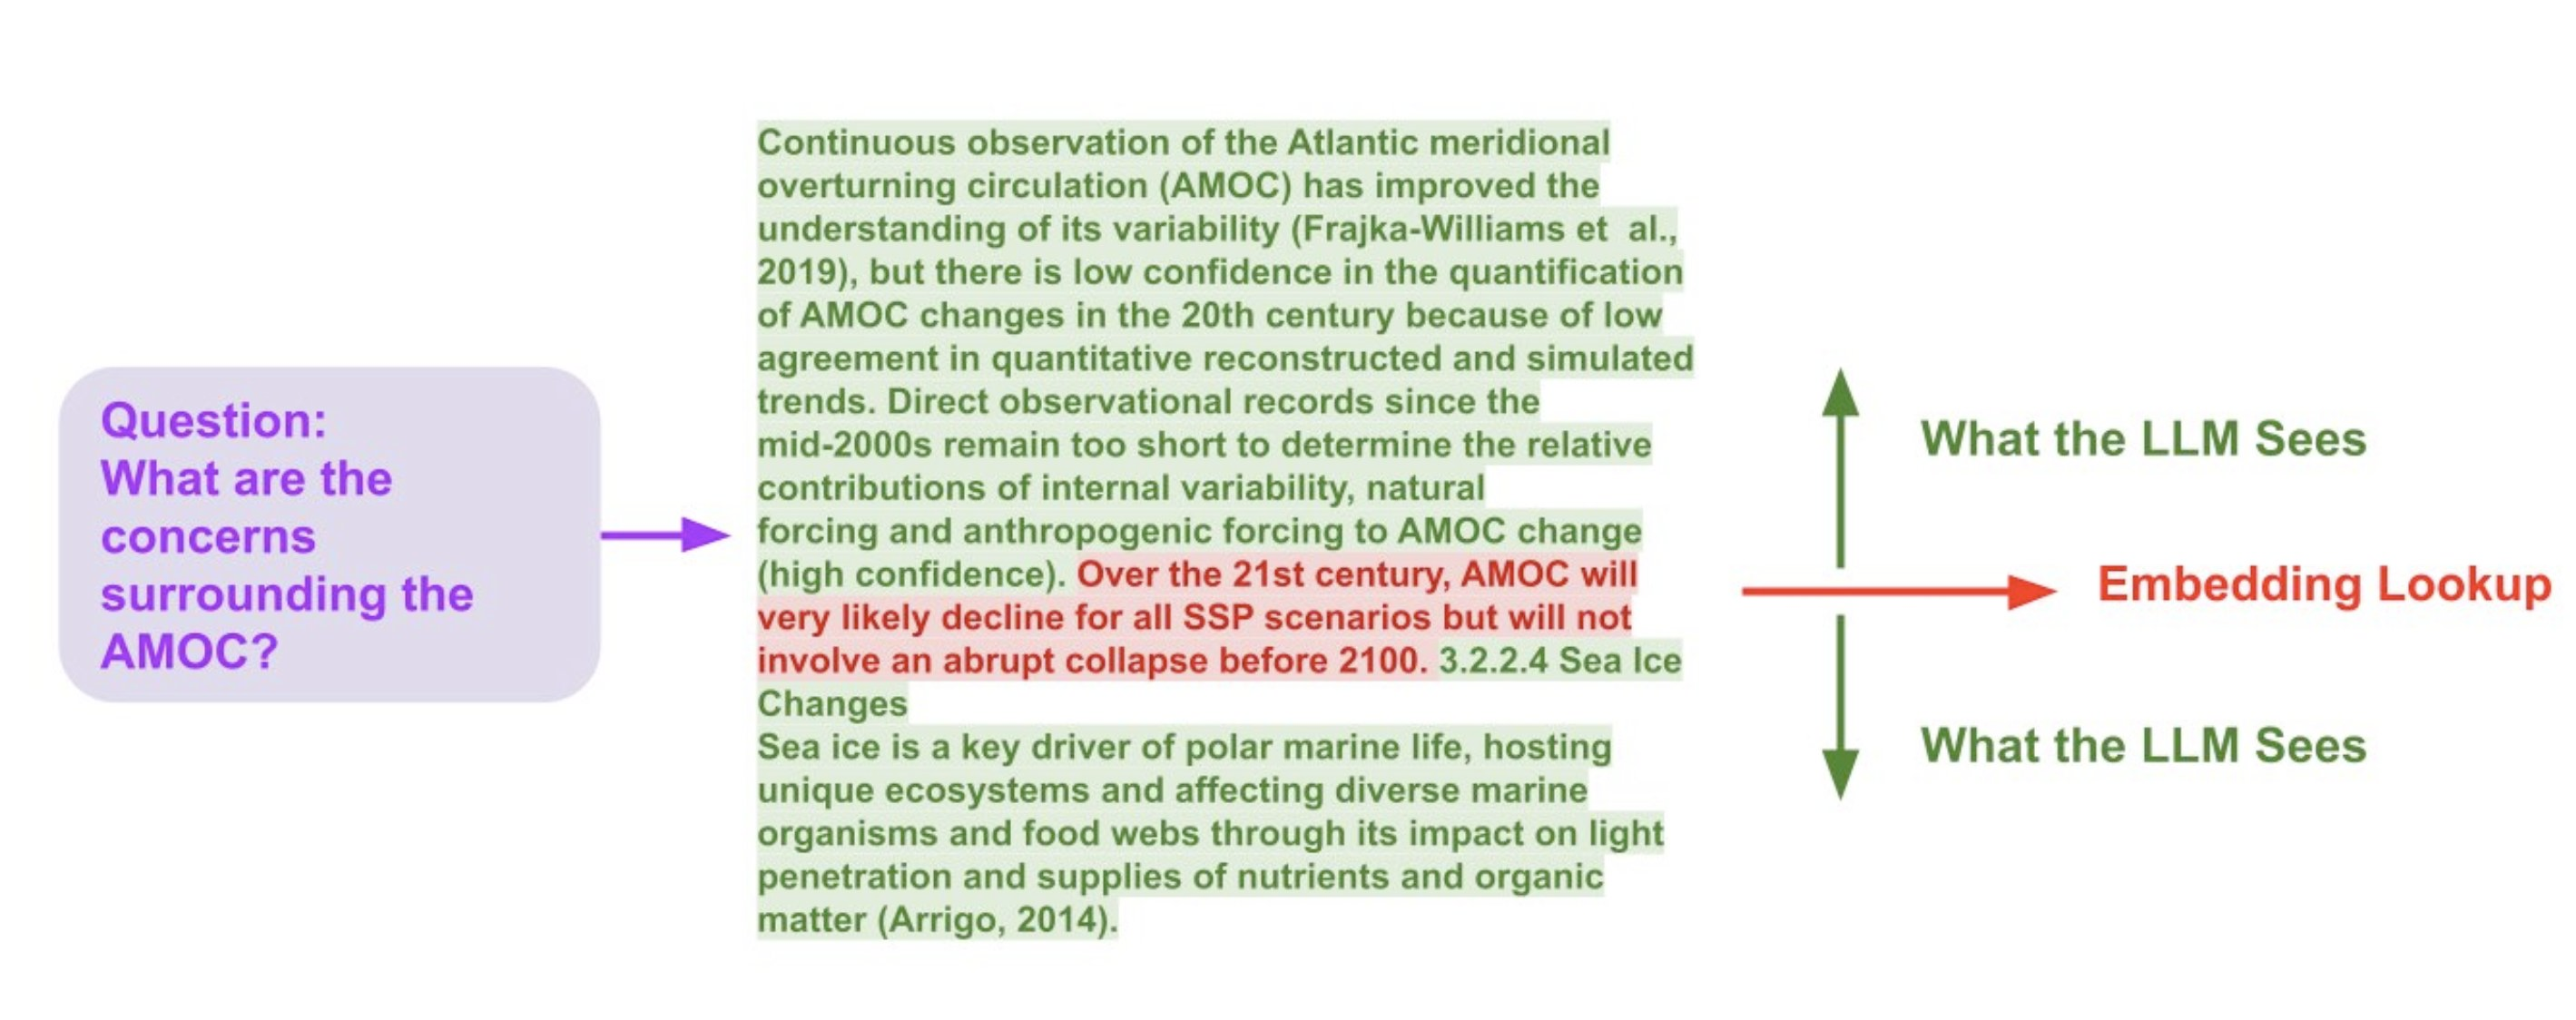
\includegraphics[width=\textwidth]{res/window-ret}
        \caption{Node sentence window replacement~\cite{liu2023tweet}}
        \label{fig:window-ret}
    \end{minipage}
\end{figure}

There is example of the \textit{SentenceWindowNodeParser} and \textit{MetadataReplacementNodePostProcessor} in the Appendix~\ref{sec:chunking:sliding-window}.

\subsubsection{Challenges and Considerations}
Several challenges and considerations are inherent in the Embedding and Retrieval Tasks:
\begin{itemize}
    \item \textbf{Multilingual Support:} Extending embedding capabilities to support multiple languages, potentially through multilingual or language-agnostic models.
    \item \textbf{Embedding Interpretability:} Balancing the trade-off between the performance of dense embeddings and the interpretability often associated with sparse representations.
    \item \textbf{Temporal Dynamics:} Addressing the challenge of embedding temporally sensitive information and ensuring retrieval mechanisms account for time-based relevance.
    \item \textbf{Scalability:} Designing the embedding and retrieval systems to efficiently handle growing volumes of data without compromising on speed or accuracy.
    \item \textbf{Ethical Considerations:} Mitigating potential biases inherent in pre-trained embedding models and ensuring fair representation across diverse topics and perspectives.
\end{itemize}

\subsection{Similarity Cutoff Strategy}\label{subsec:similarity-cutoff-strategy}
One of the most important aspects that is highlighted in the pipeline diagram is the "Similarity Cutoff Strategy," which is significant since it is responsible for filtering and prioritizing the information that is included.

This strategy likely involves:
\begin{itemize}
    \item \textbf{Threshold Definition:} Establishing a similarity threshold below which embedded chunks are considered insufficiently relevant or related to the query or context.
    \item \textbf{Similarity Metrics:} Employing appropriate similarity measures (e.g., cosine similarity, Euclidean distance) to quantify the relatedness between embedded representations.
    \item \textbf{Re-run Mechanism:} Potentially re-do the response generation process if the similarity cutoff is not met for all the documents and the response is not generated.
\end{itemize}

The Similarity Cutoff Strategy serves several critical functions:
\begin{itemize}
    \item \textbf{Noise Reduction:} Filtering out irrelevant or tangentially related information to improve the signal-to-noise ratio in subsequent processing stages.
    \item \textbf{Computational Optimization:} Reducing the volume of data processed in later stages, thereby enhancing overall system efficiency.
    \item \textbf{Relevance Enhancement:} Ensuring that only the most pertinent information is retained for query resolution and response generation.
\end{itemize}

It can be switched off if the dataset is small or if the similarity cutoff is not needed.

\section{LLMs}\label{sec:large-language-models-llms-in-the-pipeline}
\ac{LLMs} play a pivotal role in our advanced NLP pipeline, serving as the cornerstone for sophisticated information synthesis and response generation.
As illustrated in the pipeline diagram, multiple LLMs are employed, contributing to a robust and nuanced approach to question answering and information processing.

\subsection{Integration of Multiple LLMs}\label{subsec:integration-of-multiple-llms}
The pipeline incorporates multiple LLMs working in concert, a design choice that offers several significant advantages:
\begin{itemize}
    \item \textbf{Diversity of Perspectives:} By utilizing multiple models, the system can capture a broader range of interpretations and approaches to information synthesis.
    \item \textbf{Specialization:} Different LLMs may be fine-tuned or specialized for particular types of queries or domains, allowing for more targeted and accurate responses in specific contexts.
    \item \textbf{Robustness:} The multi-model approach provides redundancy and helps mitigate individual model biases or weaknesses.
    \item \textbf{Scalability:} Parallel processing of information through multiple LLMs can potentially improve the system's throughput and response time.
\end{itemize}

Implementation considerations:
\begin{itemize}
    \item \textbf{Model Selection:} Choosing a diverse set of LLMs that complement each other in terms of strengths and specializations.
    \item \textbf{Load Balancing:} Implementing efficient mechanisms to distribute workload across the available models.
    \item \textbf{Version Management:} Maintaining and updating multiple LLMs to ensure they remain current and aligned with the latest advancements in NLP.
\end{itemize}

For running open-source LLMs, we use \textit{Ollama}\footnote{\url{https://ollama.com/}}, Ollama is an open-source project that simplifies the process of setting up, running, and using large language models (LLMs) locally on your machine.
It provides a user-friendly area for managing and interacting with various LLMs, making it easier for developers and enthusiasts to experiment with AI without relying on cloud services.
Under the hood, \textit{Ollama} is just an API server written in go that serves GGUF models via llama.cpp~\footnote{\url{https://github.com/ggerganov/llama.cpp}} and a centralized hub of models/settings.

Performance Considerations and Limitations:
\begin{itemize}
    \item Performance Considerations
    \begin{itemize}
        \item Performance depends on your hardware, especially CPU and GPU capabilities.
        \item Larger models require more RAM and storage space.
        \item GPU acceleration can significantly improve inference speed.
    \end{itemize}
    \item Limitations
    \begin{itemize}
        \item Resource intensive for larger models.
        \item May not match the performance of cloud-based solutions for some use cases.
        \item Limited to models that are compatible with Ollama's framework.
    \end{itemize}
\end{itemize}

\subsection{Roles of LLMs in the Pipeline}\label{subsec:roles-of-llms-in-the-pipeline}
Based on the pipeline diagram, the LLMs serve several crucial functions:
\begin{itemize}
    \item \textbf{Information Synthesis:} Integrating and coherently combining information from various sources.
    \item \textbf{Context Processing:} Analyzing and interpreting the broader context of queries and retrieved information to generate more accurate and relevant responses.
    \item \textbf{Reasoning and Inference:} Drawing logical conclusions and making inferences based on the available information, potentially finding the correctness of the knowledge graph.
\end{itemize}

The prompt template used for RAG approach reported in Appendix~\ref{sec:prompt-templates:rag}, we use the selected chunks from the previous steps to feed the LLMs context and also provide few examples to the LLMs to generate the better response.

\section{Voting System and Conflict Resolution}\label{sec:model-diversity-and-conflict-resolution}
Our state-of-the-art pipeline for natural language processing relies heavily on the integration of many models and the deployment of procedures to resolve conflicts.
To ensure robust and trustworthy outcomes, this section covers the ways adopted to resolve disputes and harness model diversity.

\subsection{Majority Voting System}\label{subsec:majority-voting-system}
A significant aspect of the LLM integration, is the establishment of a majority voting mechanism for response creation.

This method provides numerous advantages:
\begin{itemize}
    \item \textbf{Consensus Building:} By aggregating outputs from multiple models, the system can identify areas of agreement, potentially leading to more reliable responses.
    \item \textbf{Error Mitigation:} Outlier responses or errors from individual models can be identified and potentially filtered out through the voting process.
    \item \textbf{Confidence Scoring:} The degree of consensus among models can serve as a proxy for the confidence level of the generated response.
    \item \textbf{Handling Ambiguity:} In cases where there's no clear majority, the system can potentially flag the response as uncertain or requiring further clarification.
\end{itemize}

Implementation challenges:
\begin{itemize}
    \item \textbf{Weighting Mechanism:} Determining whether all LLMs should have equal weight in the voting process or if some models should be prioritized based on their specific strengths or reliability.
    \item \textbf{Threshold Setting:} Establishing the criteria for what constitutes a "majority" and how to handle cases with no clear consensus.
    \item \textbf{Combining Diverse Outputs:} Developing methods to meaningfully aggregate potentially disparate outputs from different models into a coherent final response.
\end{itemize}
The pipeline incorporates several mechanisms for resolving conflicts that may arise from divergent model outputs:

\subsection{Conflict Resolution Strategies}\label{subsec:conflict-resolution-strategies}
As previously discussed~\ref{subsec:majority-voting-system}, the system employs a majority voting approach among LLMs to determine the most appropriate response.
This serves as a primary conflict resolution mechanism, leveraging the wisdom of the collective to mitigate individual model errors or biases.
\subsubsection{Final Judge Implementation:}
A crucial component in the conflict resolution process is the "final judge" module, as indicated in the pipeline diagram.
This element plays a pivotal role in resolving conflicts and ensuring coherence in the system's outputs.

Key aspects of the final judge implementation:
\begin{itemize}
    \item \textbf{Conflict Identification:} Detecting discrepancies or contradictions in outputs from different models.
    \item \textbf{Resolution Mechanisms:} Using predefined rules or algorithms to determine the final output based on the majority voting results.
    \item \textbf{Tie-Breaking:}Implementing strategies for scenarios where the majority voting system results in a tie or lacks a clear consensus.
    \item \textbf{Consistency Enforcement:} Ensuring that the final output maintains logical consistency and aligns with established knowledge bases.
\end{itemize}

The final judge module used a system named \textit{Adaptive Conflict Resolution}, which is an adaptive approach to conflict resolution based on the specified settings.

\subsubsection{Adaptive Conflict Resolution}
The pipeline demonstrates an adaptive approach to conflict resolution, as evidenced by the following feature:
"When two of the language models believe the answer is correct, and two believe it is wrong, we switch to a more advanced model, such as a commercial one or a model with more parameters."
There are two ways to apply this adaptive method: 1) Directly selecting paid models (e.g., GPT-4), or 2) Using a more advanced, open-source model with more parameters (e.g., Gemma2:27b).
For the second option, we use the algorithm shown in Algorithm~\ref{alg:model-selection}.
This algorithm uses the mapping between the already used and final models to select the final model.
It utilizes parameters to identify either the most stable model or the least stable model to choose based on a majority vote across the entire system.

This adaptive strategy offers several advantages:
\begin{itemize}
    \item \textbf{Escalation Mechanism:} Provides a structured approach for handling ambiguous cases where simpler resolution methods are insufficient.
    \item \textbf{Resource Optimization:} Reserves the use of more advanced (and potentially more computationally expensive) models for cases that truly require their capabilities.
    \item \textbf{Accuracy Enhancement:} Leverages more sophisticated models to resolve complex conflicts, potentially leading to higher-quality outputs in challenging scenarios.
    \item \textbf{Flexibility:} Allows for the integration of specialized or proprietary models in a targeted manner, enhancing the system's overall capabilities without relying on these models for every query.
\end{itemize}

Implementation challenges:
\begin{itemize}
    \item \textbf{Threshold Definition:} Determining the exact criteria for when to invoke the more advanced models.
    \item \textbf{Model Selection:} Choosing which advanced model to use based on the nature of the conflict and the query context.
    \item \textbf{Integration:} Ensuring smooth handover and result incorporation from the advanced models back into the main pipeline.
\end{itemize}

\begin{algorithm}
    \caption{Resolve Ties in Majority Voting System}
    \begin{algorithmic}[1]
        \Require
        \Statex $data$ - A list of dictionaries, each representing a model's response
        \Statex $finalJudger$ - A dictionary mapping file indices to final model
        \Statex $atLeast$ - A boolean flag:
        \Statex \hspace{1em} True: select model with the highest agreement score
        \Statex \hspace{1em} False: select model with the lowest agreement score

        \Procedure{ProcessFiles}{$data, finalJudger, atLeast$}
            \State $majorityValues \gets \emptyset$
            \State $keys \gets $ keys from first element of $data$
            \For{each $key$ in $keys$}
                \State $values \gets $ list of values for $key$ from all data
                \State $count \gets $ count occurrences of 1's and 0's in $values$
                \If{count of 1's $>$ count of 0's}
                    \State $majorityValues[key] \gets 1$
                \ElsIf{count of 1's $<$ count of 0's}
                \State $majorityValues[key] \gets 0$
                \Else
                    \State continue to next key
                \EndIf
            \EndFor

            \State $modelScores \gets \emptyset$
            \For{$i \gets 0$ to $|data| - 1$}
                \State $trueCount \gets 0$
                \For{each $(k, v)$ in $data[i]$}
                    \If{$majorityValues[k] = v$}
                        \State $trueCount \gets trueCount + 1$
                    \EndIf
                \EndFor
                \State Add $(i, trueCount)$ to $modelScores$
            \EndFor

            \If{$atLeast$ is True}
                \State $maxScore \gets $ maximum score in $modelScores$
                \State $candidates \gets $ indices with score equal to $maxScore$
            \Else
                \State $minScore \gets $ minimum score in $modelScores$
                \State $candidates \gets $ indices with score equal to $minScore$
            \EndIf

            \State $chosenIndex \gets $ random choice from $candidates$
            \State \Return $finalJudger[chosenIndex]$
        \EndProcedure
    \end{algorithmic}\label{alg:model-selection}
\end{algorithm}

\section{Pipeline Flow and Decision Points}\label{sec:pipeline-flow-and-decision-points}
The architecture of our pipeline is characterized by a sophisticated flow of information and a series of critical decision points.
This structure enables the system to process complex queries, retrieve and synthesize relevant information, and generate accurate responses.
This section provides a comprehensive analysis of the pipeline's flow and the key decision points that guide the processing of information.

The pipeline flow can be broadly categorized into several main stages, each with its own set of processes and decision points:
\begin{itemize}
    \item Input Processing and Query Generation
    \item Information Retrieval and Enrichment
    \item Embedding and Relevance Assessment
    \item Multi-Model Processing and Synthesis
    \item Conflict Resolution and Final Output Generation
\end{itemize}
Let's examine each of these stages in detail in table~\ref{tab:pipeline-decision-points}, focusing on the flow of information and the critical decision points within each.
\begin{table}[ht!]
    \noindent
    \resizebox{\textwidth}{!}{
        \begin{tabular}{lp{11cm}}
            \toprule
            \textbf{Component} & \textbf{Decision Point} \\
            \midrule
            \multicolumn{2}{c}{\colorbox{pink}{\textit{Input Processing and Query Generation}}} \\
            Knowledge Graph Dataset Integration & Extent and nature of knowledge graph integration based on input complexity. \\
            Human-Understandable Text Generation & Selection of the most appropriate natural language generation technique based on input and context. \\
            Question Generation & Assessment of the quality and relevance of generated questions. \\
            Cross-Encoder for Query Relevance & Determination of whether the top question score exceeds the upper threshold. \\
            \hdashline
            \multicolumn{2}{c}{\colorbox{pink}{\textit{Information Retrieval and Enrichment}}}  \\
            Information Source Selection & Determining the most relevant and reliable sources for information retrieval. \\
            Google Search Integration & Balancing between the breadth of search (number of questions submitted) and depth (number of results retrieved). \\
            Process and Extract Links & Determining the relevance and quality of extracted information for inclusion in the data pool. \\
            Data Pool Creation & Structuring the data pool for optimal accessibility in subsequent stages. \\
            \hdashline
            \multicolumn{2}{c}{\colorbox{pink}{\textit{Embedding and Relevance Assessment}}} \\
            Embedding for Retrieval Tasks & Selection of the most appropriate embedding technique based on the nature of the data. \\
            Similarity Cutoff Strategy & Determination of the similarity cutoff threshold. \\
            Context Processing & Determining the optimal chunk size and processing method. \\
            \hdashline
            \multicolumn{2}{c}{\colorbox{pink}{\textit{Multi-Model Processing and Synthesis}}} \\
            Parallel LLM Processing & Allocation of specific tasks or aspects of the query to different models based on their strengths. \\
            Synthesis of Information & Determination of the method of synthesis (e.g., concatenation, abstraction, or hybrid approaches). \\
            Majority Voting System & Assessment of the level of agreement among models. \\
            \hdashline
            \multicolumn{2}{c}{\colorbox{pink}{\textit{Conflict Resolution and Final Output Generation}}} \\
            Conflict Identification & Determination of the threshold for what constitutes a significant conflict requiring resolution. \\
            Adaptive Model Selection & When two models believe the answer is correct and two believe it's wrong, switching to a more advanced model. \\
            Selection of Commercial Models & Choose the commercial model based on the user specified settings. \\
            Final Judge Implementation & Determination of the final response based on aggregated model outputs and conflict resolution results. \\
            Response Generation & Selection of the most appropriate format and level of detail for the response. \\
            \bottomrule
        \end{tabular}}\caption{Comprenhensive list of decision points in the pipeline flow.}
    \label{tab:pipeline-decision-points}
\end{table}

Several challenges and considerations are associated with managing the pipeline flow and decision points:
\begin{itemize}
    \item \textbf{Computational Efficiency:} Balancing the depth of processing at each stage with the need for timely responses.
    \item \textbf{Error Propagation:} Ensuring that errors or biases introduced at early stages don't disproportionately affect the final output.
    \item \textbf{Adaptability:} Designing decision points that can adapt to different query types and complexity levels.
    \item \textbf{Transparency:} Maintaining traceability of decisions made throughout the pipeline for accountability and debugging purposes.
    \item \textbf{Scalability:} Ensuring that the pipeline can handle increasing query volumes without significant degradation in performance or accuracy.
\end{itemize}

In conclusion, the Pipeline Flow and Decision Points represent a complex yet well-structured approach to natural language processing and question answering.
By implementing a series of carefully designed stages and critical decision points, the system aims to process information in a manner that maximizes accuracy, relevance, and reliability.
The adaptive nature of the pipeline, particularly in its approach to conflict resolution and model selection, demonstrates a commitment to handling a wide range of query complexities and scenarios.
However, the intricate nature of this flow also underscores the importance of ongoing optimization, monitoring, and refinement to ensure that the system continues to perform effectively and ethically in the face of evolving challenges and requirements in the field of AI and natural language processing.
\section{Performance Report}\label{sec:performance-report}
In Tables~\ref{tab:pipeline-performance-report},~\ref{tab:pipeline-performance-report-2}, we provide a detailed performance report, highlighting key metrics that demonstrate the pipeline's efficiency.
Other sections of the pipeline, such as RAG and conflict resolution mechanisms, will be evaluated in future chapters.
\begin{table}[ht!]
    \noindent
    \resizebox{\textwidth}{!}{
        \begin{tabular}{lcc}
            \toprule
            \textbf{Task} & \textbf{Avg. Request Duration} & \textbf{Avg. tokens per request} \\
            \midrule
            Human understandable text~\ref{subsec:human-understandable-text-generation} & 1.3164 sec & 343.16 \\
            Question Generation~\ref{subsec:question-formulation-techniques} & 9.6076 sec & 672.58 \\
            \bottomrule
        \end{tabular}}
    \caption{Performance of our LLM applications in production, generated by Openlit~\footnote{\url{https://openlit.io/}} with \textit{Gemma2} model.}
    \label{tab:pipeline-performance-report}
\end{table}

\begin{table}[ht!]
%    \noindent
    \centering
    \begin{tabular}{lc}
        \toprule
        \textbf{Task} & \textbf{Avg. Duration} \\
        \midrule
        Sorting the questions by similarity~\ref{subsec:cross-encoder-for-query-relevance-scoring} & 0.013 sec \\
        Get documents (Google pages)~\ref{subsec:google-search-integration} & 3.6 sec \\
        Fetch documents for each triple~\ref{subsec:process-and-extract-links} & 350 sec \\
        \bottomrule
    \end{tabular}
    \caption{Performance of our Information Retrieval Mechanisms.}
    \label{tab:pipeline-performance-report-2}
\end{table}



\section{Ethical Considerations and Limitations}\label{sec:ethical-considerations-and-limitations}
The development and deployment of advanced pipelines, such as the one described in this thesis, necessitate a thorough examination of ethical considerations and an acknowledgment of system limitations.
This section explores the ethical implications of our fact-checking system and discusses its inherent constraints.

\subsection{Ethical Considerations}\label{subsec:ethical-considerations}
While the pipeline diagram does not explicitly highlight ethical components, several aspects of the system raise important ethical considerations:

\subsubsection{Misinformation and Harmful Content}\label{subsubsec:misinformation-and-harmful-content}
The system's ability to synthesize information from various sources poses risks related to misinformation:
\begin{itemize}
    \item \textbf{Propagation of False Information:} Potential for the system to inadvertently spread misinformation present in retrieved data.
    \item \textbf{Generation of Harmful Content:} Risk of producing responses that could be considered harmful, offensive, or inappropriate.
\end{itemize}

%Mitigation Strategies:
%\begin{itemize}
%    \item Implementation of fact-checking mechanisms and reliable source prioritization.
%    \item Content filtering systems to detect and prevent the generation of harmful or inappropriate responses.
%    \item Regular updates to the system to address emerging misinformation trends.
%\end{itemize}

\subsubsection{Environmental Considerations}\label{subsubsec:environmental-considerations}
The computational resources required to run multiple LLMs and process large volumes of data raise environmental concerns:
\begin{itemize}
    \item \textbf{Energy Consumption:} High energy usage associated with running complex AI models and large-scale data processing.
    \item \textbf{Carbon Footprint:} Environmental impact of the infrastructure required to support the pipeline.
\end{itemize}

%Mitigation Strategies:
%\begin{itemize}
%    \item Optimization of model efficiency and resource utilization.
%    \item Exploration of more energy-efficient hardware and green computing practices.
%    \item Consideration of the trade-offs between model complexity and environmental impact.
%\end{itemize}

\subsection{Limitations}\label{subsec:limitations}
Understanding and acknowledging the limitations of the system is crucial for ethical deployment and user trust:

\begin{table}[h!]
    \noindent
    \resizebox{\textwidth}{!}{
        \begin{tabular}{lp{11cm}}
            \toprule
            \textbf{Limitation} & \textbf{Description} \\
            \midrule
            \multicolumn{2}{c}{\colorbox{pink}{\textit{Scope of Knowledge}}} \\
            Temporal Limitations & The system's knowledge base and models have a cutoff date, potentially leading to outdated information. \\
            Domain Specificity & Gaps in specialized or niche areas of knowledge may limit performance. \\
            \hdashline
            \multicolumn{2}{c}{\colorbox{pink}{\textit{Language and Cultural Limitations}}} \\
            Language Coverage & Biases towards languages well-represented in training data, challenges in handling less common languages. \\
            Cultural Context & Limitations in understanding and responding to culturally specific queries or contexts. \\
            \hdashline
            \multicolumn{2}{c}{\colorbox{pink}{\textit{Reasoning and Inference Capabilities}}} \\
            Complex Reasoning & Challenges in handling queries requiring advanced logical reasoning or domain-specific expertise. \\
            Causal Understanding & Difficulties in inferring causal relationships. \\
            \hdashline
            \multicolumn{2}{c}{\colorbox{pink}{\textit{Handling of Ambiguity and Context}}} \\
            Contextual Nuances & Difficulties in capturing subtle contextual cues that humans naturally understand. \\
            Disambiguation & Challenges in resolving ambiguities in queries without additional user input. \\
            \hdashline
            \multicolumn{2}{c}{\colorbox{pink}{\textit{Real-time Adaptation}}} \\
            Static Knowledge Base & Limitations in adapting to real-time changes without system updates. \\
            Learning from Interactions & Inability to learn and improve from individual user interactions due to privacy and architectural constraints. \\
            \bottomrule
            \end{tabular}}\caption{Limitions of the pipeline.}
    \label{tab:pipeline-limitations}
\end{table}

% TODO: MAYBE FUTURE WORK
%3.10.3 Addressing Ethical Concerns and Limitations
%To address these ethical considerations and limitations, several approaches can be implemented:
%
%Ethical Oversight:
%
%Establishment of an ethics board to guide development and deployment decisions.
%Regular ethical audits of the system's performance and impacts.
%
%
%User Education:
%
%Clear communication to users about the system's capabilities, limitations, and potential biases.
%Promotion of critical thinking and fact-checking when using AI-generated information.
%
%
%Continuous Improvement:
%
%Ongoing research and development to address identified limitations and ethical concerns.
%Regular updates to the Knowledge Graph Dataset and model fine-tuning to improve accuracy and reduce biases.
%
%
%Collaborative Development:
%
%Engagement with diverse stakeholders, including ethicists, domain experts, and potential user groups, in the ongoing development and refinement of the system.
%
%
%Regulatory Compliance:
%
%Proactive alignment with emerging AI regulations and ethical guidelines.
%Participation in industry initiatives for responsible AI development.
%
%
%
%In conclusion, while the advanced natural language processing pipeline presented in this thesis offers powerful capabilities for information retrieval and question answering, it also comes with significant ethical considerations and inherent limitations. Acknowledging these challenges is crucial for responsible development and deployment. By actively addressing ethical concerns, transparently communicating limitations, and continuously striving for improvement, we can work towards a system that not only advances the field of AI but also aligns with societal values and ethical standards. The complexity of these considerations underscores the need for ongoing dialogue and collaboration between technologists, ethicists, policymakers, and the broader public to ensure that AI systems like this pipeline contribute positively to society while minimizing potential harms.


% TODO: FUTURE WORK MAYBE
%\subsection{Integration with Other Pipeline Components}\label{subsec:integration-with-other-pipeline-components}
%
%The LLMs interact closely with other components of the pipeline:
%
%Input from Embedding and Retrieval: The LLMs receive contextualized, relevant information chunks from the embedding and retrieval stages, ensuring they have access to the most pertinent data for response generation.
%Feedback to Information Retrieval: The LLMs may potentially provide feedback to refine or guide further information retrieval based on initial processing results.
%Interface with Final Judge: As indicated in the diagram, the output from the LLM majority voting system feeds into a "final judge" component, suggesting an additional layer of quality control or decision-making.
%
%3.6.5 Challenges and Considerations
%
%Several challenges and ethical considerations are associated with the use of LLMs in the pipeline:
%
%Bias Mitigation: Addressing and mitigating potential biases inherent in the training data of LLMs.
%Explainability: Developing methods to provide transparency and explanations for the reasoning behind generated responses, especially crucial in a multi-model voting system.
%Consistency: Ensuring consistency in responses across multiple queries and different combinations of activated LLMs.
%Computational Resources: Managing the significant computational requirements of running multiple LLMs concurrently.
%Privacy and Data Handling: Ensuring that sensitive information is handled appropriately and that the LLMs do not inadvertently reveal private data.
%Ethical Use: Implementing safeguards to prevent the generation of harmful, false, or misleading content.
%
%3.6.6 Future Directions
%
%The integration of LLMs in the pipeline opens up several avenues for future enhancements:
%
%Dynamic Model Selection: Implementing systems that can dynamically select the most appropriate combination of LLMs based on the specific query and context.
%Continuous Learning: Exploring methods for ongoing fine-tuning or adaptation of the LLMs based on user interactions and feedback, while maintaining ethical boundaries.
%Multi-modal Integration: Expanding the capabilities of the pipeline to incorporate LLMs that can process and generate multi-modal content (text, images, audio).
%Enhanced Reasoning Capabilities: Developing techniques to improve the logical reasoning and inference capabilities of the LLMs, potentially through integration with symbolic AI approaches.
%
%In conclusion, the incorporation of multiple Large Language Models into the pipeline represents a sophisticated approach to natural language processing and question answering. By leveraging the strengths of diverse models and implementing a majority voting system, the pipeline aims to generate more accurate, nuanced, and reliable responses. This approach, while powerful, also necessitates careful consideration of ethical implications and ongoing efforts to address challenges related to bias, consistency, and explainability. The central role of LLMs in this pipeline underscores their transformative potential in advancing the field of artificial intelligence and natural language understanding.
%

    \chapter{Empirical Evaluation}\label{ch:empirical-evaluation}

\section{Dataset Analysis}\label{sec:empirical-evaluation:dataset-analysis}
This section presents an analysis of the three datasets used in our empirical evaluation: \textit{FactBench}, \textit{YAGO}, and \textit{DBpedia}.
Each dataset offers unique characteristics and challenges, providing a comprehensive basis for assessing our knowledge graph fact verification system.
\subsection{FactBench Dataset}\label{subsec:empirical-evaluation:dataset-analysis:factbench}
\textit{FactBench} is a multilingual dataset specifically designed for fact-checking in knowledge graphs~\footnote{\url{https://github.com/DeFacto/FactBench}}~\cite{GERBER201585}.
It comprises 2,800 facts, 1.500 true and 1.300 false, across three languages: English, German, and French.
The dataset covers various domains, including geography, politics, and entertainment.
The data was automatically extracted from Wikipedia\footnote{\url{https://www.wikipedia.org/}} (DBpedia respectively) and Freebase\footnote{\url{https://developers.google.com/freebase}}.

To obtain positive examples, the authors leverages facts from both DBpedia and Freebase.
For each property under consideration, they generated these examples by issuing either a SPARQL (for DBpedia) or MQL (for Freebase) query.
They then selected the top 150 results.
In Freebase, results are ranked using an internal relevance score, while in \textit{DBpedia}, the results are sorted by the number of inbound links to the resource’s corresponding Wikipedia page.
In total, 1500 correct statements were collected, with 750 allocated to both the test and training sets, ensuring that each relation had 150 positive facts equally distributed between the test and training sets.

For generating incorrect facts (negative examples), the authors modified correct ones while adhering to domain and range constraints.
To ensure that the negative examples closely resemble true statements (\ie, meaningful triples), the team altered the positive examples while still adhering to domain and range restrictions.
Given a triple (s, p, o) and its timespan (from, to) from the knowledge base, they used different methods to generate sets of negative examples.
These methods include modifying the subject, object, both subject and object, or the property.
Additionally, they included random modifications, a 20\% mix of these methods, and variations in the date.

We don't consider the time aspect in our evaluation, as our system is not designed to handle time-sensitive issues.
We consider a configuration where incorrect facts are a mix produced using different negative example generation strategies, resulting in a ground-truth accuracy of $\mu$ = 0.54.
Key characteristics of \textit{FactBench} include:
\begin{itemize}
    \item Multilingual support (English, German, and French)
    \item Diverse fact types, including domain-specific and temporal facts
    \item Manually curated for high-quality ground truth
\end{itemize}

In our analysis, we found that \textit{FactBench} presents a balanced challenge for our system, with a mix of straightforward and complex fact verification tasks.
\subsection{YAGO Dataset}\label{subsec:empirical-evaluation:dataset-analysis:yago}
YAGO (Yet Another Great Ontology) is a large-scale knowledge base derived from Wikipedia, WordNet~\footnote{\url{https://wordnet.princeton.edu/}}, and GeoNames~\footnote{\url{https://www.geonames.org/}}.
For our evaluation, we use \textit{YAGO2-sample}~\footnote{\url{https://aclanthology.org/attachments/D17-1183.Attachment.zip}}~\cite{ojha-talukdar-2017-kgeval}, a subset of the full YAGO2 knowledge graph derived from AMIE horn clauses~\cite{Yago_AMIE}.
This sample consists of 1,386 beliefs spanning 16 unique predicates.

Key characteristics of the \textit{YAGO} dataset in our evaluation include:
\begin{itemize}
    \item High accuracy: The gold standard accuracy of the \textit{YAGO2-sample} is 99.20\%, indicating a very high-quality dataset.
    \item Diverse predicates: The sample covers 16 different predicates, allowing for evaluation across a range of relationship types.
    \item Balanced distribution: Unlike domain-specific datasets, \textit{YAGO2-sample} covers a broad range of topics, reflecting the diverse nature of Wikipedia.
\end{itemize}

The high accuracy of the \textit{YAGO2-sample} presents a unique challenge for our evaluation system.
\subsection{DBpedia Dataset}\label{subsec:empirical-evaluation:dataset-analysis:dbpedia}
\textit{DBpedia} serves as a comprehensive, large-scale knowledge base derived from Wikipedia, offering structured information about millions of entities.
For our evaluation, we utilize \textit{DBpedia} version 2015-10 which contains approximately 6.2M entities and 1.1B triplets.
Following Marchesin et al.'s approach~\cite{Marchesin_Silvello_Alonso_2024} to entity-oriented research, several filtering criteria were applied to ensure high-quality data for evaluation.

The analysis was restricted to subject entities that include both: 1) rdfs:label predicate and 2) rdfs:comment predicate

Additionally, they focused exclusively on A-Box triplets (assertional knowledge) while excluding T-Box triplets (terminological knowledge).
The T-Box encompasses ontological entities and relationships, while A-Box contains the actual assertions that need verification.
After applying these filters, their working dataset consisted 4.6M entities with 170M triplets.

From this filtered dataset, they conducted a comprehensive annotation study on 9,930 facts, which were carefully selected to represent diverse types of relationships and knowledge domains within \textit{DBpedia}.
To ensure annotation quality, Marchesin et al. implemented several measures:
\begin{itemize}
    \item Multiple annotators per fact (minimum of three annotations per triplet)
    \item Expert consensus requirement for final labels
    \item Binary validation approach treating all incorrect facts equally regardless of error type
    \item Documented agreement rates between expert annotators (77\% agreement with Cohen's κ score of 0.51)
    \item Third-party resolution for 82\% of initial disagreements
\end{itemize}

The dataset was carefully curated to ensure a manageable yet representative evaluation set, derived from the vast scale of \textit{DBpedia}.
By utilizing this curated subset of \textit{DBpedia}, we benefit from a balance between the richness of a real-world knowledge graph and the practicality required for thorough empirical evaluation.
For our evaluation system, we use subset of this annotated dataset, by removing facts with \textit{<UNK>} labels, resulting in 9,344 facts.

\paragraph{Dataset Summary:}\label{par:summary}
To conclude, our empirical evaluation utilizes three distinct datasets: \textit{FactBench}, \textit{YAGO}, and \textit{DBpedia}.
Each dataset offers unique characteristics that allow us to assess our knowledge graph veracity framework across diverse scenarios.
Table~\ref{tab:dataset-summary} summarizes the key features of these datasets:

\begin{table}[h!]
    \centering
    \caption{Statistical summary of FactBench, YAGO, and DBpedia datasets}
    \begin{tabular}{lccc}
        \toprule
        & \textbf{FactBench} & \textbf{YAGO} & \textbf{DBpedia} \\
        \midrule
        Num. of Facts & 2,800 & 1,386 & 9,344 \\
        Num. of Predicates & 10 & 16 & 1,092 \\
%        Query-Entity Pairs & N/A & N/A & N/A \\
        Avg. Facts per Entity & 2.42 & 1.69 & 3.18 \\
        Gold Accuracy ($\mu$) & 0.54 & 0.99 & 0.85 \\
        \bottomrule
    \end{tabular}
    \label{tab:dataset-summary}
\end{table}

\textit{FactBench} provides a good distribution of true and false statements across multiple domains, offering a robust testbed for fact verification.
\textit{YAGO}, with its high accuracy, challenges our framework to detect subtle inaccuracies in an otherwise highly reliable knowledge graph.
The \textit{DBpedia} subset, curated specifically for entity-oriented search tasks, allows us to evaluate our framework in the context of query-dependent fact checking.
This diverse selection of datasets enables a comprehensive evaluation of our veracity estimation framework.

\section{Candidate Models}\label{sec:empirical-evaluation:candidate-models}
\subsection{Gemma2}\label{subsec:empirical-evaluation:candidate-models:gemma2}
Gemma is a family of lightweight, state-of-the-art open models from Google, built from the same research and technology used to create the Gemini models~\footnote{\url{https://deepmind.google/technologies/gemini/#introduction}}.
They are text-to-text, decoder-only large language models, available in English, with open weights for both pre-trained variants and instruction-tuned variants.
Gemma 2 implements a similar architecture to the original Gemma model, with a few key differences.
The model alternates between local sliding window attention with a 4096-token span and global attention with an 8192-token span in alternate layers.
Logits are capped within a specified range to stabilize the values during attention and final layers, with soft\_cap set to 50 for self-attention layers and 30 for the final layer.
RMSNorm is used for normalization in transformer sub-layers, and \ac{GQA} with two groups enhances inference speed without sacrificing performance.
This hybrid approach aims to balance efficiency with the ability to capture long-range dependencies in the input.

We selected the \textit{Gemma2-9B} model for our evaluation, which has 9 billion parameters.
The 9B model learns from a larger teacher model during initial training in pre-training and use on-policy distillation to refine its performance post-training.
This approach allows \textit{Gemma2-9B} to capture the knowledge and capabilities of the larger model while maintaining a more compact size.
As a result, \textit{Gemma2-9B} delivers competitive performance relative to models 2-3 times its size, making it an attractive choice for applications with computational constraints.

\subsection{Qwen2.5}\label{subsec:empirical-evaluation:candidate-models:qwen2.5}
\textit{Qwen2.5} is the latest series of Qwen LLMs~\cite{qwen2}.
For \textit{Qwen2.5}, Alibaba Cloud~\footnote{\url{https://www.alibabacloud.com/en?_p_lc=7}} release a number of base language models and instruction-tuned language models ranging from 0.5 to 72 billion parameters.
All models are pre-trained on our latest large-scale dataset, encompassing up to 18 trillion tokens.
Compared to \textit{Qwen2}, \textit{Qwen2.5} has acquired significantly more knowledge and has greatly improved capabilities in coding and mathematics.
Additionally, the new models achieve significant improvements in instruction following, generating long texts (over 8K tokens), understanding structured data (\eg, tables), and generating structured outputs especially JSON.
\textit{Qwen2.5} models are generally more resilient to the diversity of system prompts, enhancing role-play implementation and condition-setting for chatbots.
Like \textit{Qwen2}, the \textit{Qwen2.5} language models support up to 128K tokens and can generate up to 8K tokens.
They also maintain multilingual support for over 29 languages~\cite{qwen2.5}.

We selected the \textit{Qwen2.5-7b} model for our evaluation, which has 7 billion parameters.

\subsection{Llama3.1}\label{subsec:empirical-evaluation:candidate-models:llama3.1}
The Meta \textit{Llama3.1} collection of multilingual LLMs is a collection of pre-trained and instruction tuned generative models in 8B, 70B and 405B sizes (text in/text out).
The \textit{Llama3.1} instruction tuned text only models (8B, 70B, 405B) are optimized for multilingual dialogue use cases and outperform many of the available open source and closed chat models on common industry benchmarks.

\textit{Llama3.1} is an auto-regressive language model that uses an optimized transformer architecture.
\textit{Llama3.1} was pre-trained on ~15 trillion tokens of data.
In post-training The models produced by doing several rounds of alignment on top of the pre-trained model.
Each round involves \ac{SFT}, \ac{RS}, and \ac{DPO}.
Meta use synthetic data generation to produce the vast majority of our SFT examples, iterating multiple times to produce higher and higher quality synthetic data across all capabilities.
Additionally, they invest in multiple data processing techniques to filter this synthetic data to the highest quality.
This enables model to scale the amount of fine-tuning data across capabilities.
Compared to previous versions of Llama, developers improved both the quantity and quality of the data we use for pre and post-training.
These improvements include the development of more careful pre-processing and curation pipelines for pre-training data, the development of more rigorous quality assurance, and filtering approaches for post-training data~\cite{dubey2024llama3herdmodels,meta2023llama3}.

We selected the \textit{Llama3.1-8b} model for our evaluation, which has 8 billion parameters.

\subsection{Mistral}\label{subsec:empirical-evaluation:candidate-models:mistral}
The \textit{Mistral} model, released by Mistral AI~\footnote{\url{https://mistral.ai/}}, is a high-performance LLM, designed to outperform larger models in efficiency and effectiveness.
With innovations such as \ac{GQA} and \ac{SWA}, Mistral offers faster inference and better handling of long sequences, reducing computation costs while maintaining high performance~\cite{jiang2023mistral7b,mistral7b_2023}.

We selected the \textit{Mistral-7b} model for our evaluation, which has 7.3 billion parameters, its structure allows it to be both cost-effective and memory efficient, making it suitable for a wide variety of real-world applications

\paragraph{Candidate Model Summary:}\label{par:summary2}
The selection of candidate models for our system was guided by the need for diversity, efficiency, and reliability in processing fact verification tasks within knowledge graphs.
We chose \textit{Gemma2}, \textit{Qwen2.5}, \textit{Llama3.1}, and \textit{Mistral} for their specific strengths in handling diverse linguistic queries, reasoning capabilities, and compatibility with RAG pipelines.
Each of these models brings unique advantages to our verification framework, as summarized in Table~\ref{tab:candidate_models}.

\begin{table}[h!]
    \footnotesize
    \caption{Summary of key strengths of selected candidate LLMs for knowledge graph fact verification.}
    \begin{xltabular}{\linewidth}{cp{3.6cm}X}
        \toprule
        \textbf{Model} & \textbf{Key Strengths} & \textbf{Description} \\
        \midrule
        \multirow{3}{*}{Gemma2} & \multirow{3}{*}{\shortstack{Dense Retrieval \\\& Query Processing}} & Optimized for dense retrieval tasks, Gemma2 processes complex linguistic structures, making it well-suited for entity-rich query generation and document ranking. \\
        \hline
        \multirow{4}{*}{Qwen2.5} & \multirow{4}{*}{\shortstack{Logical Reasoning \\\& Prompt Efficiency}} & Excels in reasoning tasks with minimal prompting. Its accuracy in logical inference supports consistent veracity assessments, especially for ambiguous or conflicting evidence. \\
        \hline
        \multirow{5}{*}{Llama3.1} & \multirow{5}{*}{Efficiency \& Versatility} & Offers a balance of efficiency and accuracy, with robust performance across fact-checking benchmarks. Llama3.1's lower computational demands ensure responsive processing without compromising output quality. \\
        \hline
        \multirow{4}{*}{Mistral} & \multirow{4}{*}{\shortstack{Context Sensitivity \\\& Interpretability}} & Known for nuanced, context-driven outputs and interpretability. Mistral’s language generation capabilities provide clear, human-like explanations, making it ideal for understanding the facts like a human. \\
        \bottomrule
    \end{xltabular}
    \label{tab:candidate_models}
\end{table}

For model selection, we can choose either instruction-tuned and quantized models with similar architectures or with different architectures.
Here, we opted for models with varied architectures to make the ensemble more versatile and capable of handling a wide range of query scenarios.
Using diverse models in the ensemble offers a balanced approach to complex fact verification tasks across knowledge graphs.
This multi-model setup enhances adaptability and reliability, allowing the system to respond accurately to diverse verification scenarios, even when they differ in nature.

\section{Experimental Setup}\label{sec:empirical-evaluation:experimental-setup}
\subsection{Performance Metrics and Evaluation}\label{subsec:empirical-evaluation:experimental-setup:performance-metrics-and-evaluation}
Performance metrics are essential in assessing the efficacy, efficiency, and reliability of a system or model.
The selection of metrics mostly depends on the characteristics of the task, the data, and the objectives.
This section emphasizes the principal performance metrics typically employed in systems utilizing LLMs, information retrieval, and various machine learning tasks.
\paragraph{Correct and Incorrect Criteria:}
The system incorporates explicit CORRECT and INCORRECT states, indicating a binary evaluation mechanism for overall performance.
This fundamental assessment provides a clear, high-level indication of the system's success in handling queries.
\paragraph{Relevance and Accuracy Metrics:}
The evaluation of a fact-checking system typically involves assessing both the correctness and relevance of responses.

Potential metrics include:
\begin{itemize}
    \item \textbf{F1 Score:} The harmonic mean of precision and recall, providing a balanced measure of accuracy.
    \item \textbf{Accuracy:} The proportion of correct responses generated by the system.
\end{itemize}
\paragraph{Latency and Efficiency Measures:}
Given the complexity of the pipeline, evaluating its operational efficiency is crucial:
\begin{itemize}
    \item \textbf{Response Time:} Measuring the end-to-end time from query input to response generation.
    \item \textbf{Component-wise Latency:} Assessing the processing time of individual pipeline components (\eg, embedding generation, LLM processing). Fully reported in ablation study in chapter~\ref{ch:ablation} and performance report in section~\ref{sec:performance-report}.
    \item \textbf{Cost Efficiency:} Evaluating the cost-effectiveness of the pipeline in terms of computational resources and infrastructure by reporting the average token used per query.
\end{itemize}

\paragraph{Consistency Evaluation:}
The use of multiple models and a conflict resolution mechanism necessitates specific evaluation of output consistency:

\begin{itemize}
    \item \textbf{Stability Across Models:} Assessing the consistency of responses generated by different LLMs for the same query, refer to Algorithm~\ref{alg:stability-across-queries}.
\end{itemize}
\begin{algorithm}
    \footnotesize
    \caption{Calculate Model Consistency Per Model}
    \begin{algorithmic}[1]
        \Procedure{ModelStabilityCal}{$models$} \Comment{Containing binary results}
            \State $m\_len \gets \text{length}(models)$, $stabilityScores \gets []$

            \For{$i \gets 0$ to $m\_len - 1$}
                \State $m1 \gets models[i]$, $mStabilities \gets []$

                \For{$j \gets 0$ to $m\_len - 1$}
                    \If{$i \neq j$}
                        \State $m2 \gets models[j]$, $matchCount \gets 0$
                        \State $totPreds \gets \text{length}(m1)$

                        \For{$k \gets 0$ to $totalPredictions - 1$}
                            \If{$m1[k] = m2[k]$}
                                \State $matchCount \gets matchCount + 1$
                            \EndIf
                        \EndFor

                        \State $mStabilities$ \gets $\dfrac{matchCount}{totPreds}$ \Comment{Append the stability score}
                    \EndIf
                \EndFor

                \State $stabilityScores[i] \gets \text{mean}(mStabilities)$
            \EndFor

            \State \Return $stabilityScores$ \Comment{Dictionary with model stability scores}
        \EndProcedure
    \end{algorithmic}
    \label{alg:stability-across-queries}
\end{algorithm}

\subsection{System Configurations}\label{subsec:empirical-evaluation:experimental-setup:system-configurations}
The system configurations are selected based on the best results obtained from black-box testing the pipeline through a series of experiments, detailed in chapter~\ref{ch:ablation}.
Table~\ref{tab:system-configurations} summarizes the key system configurations used in our empirical evaluation.

{
    \noindent
    \centering
    \footnotesize
    \begin{tabularx}{\linewidth}{lp{2.9cm}X}
        \caption{System configurations for empirical evaluation} \\
        \toprule
        \textbf{Section} & \textbf{Parameter} & \textbf{Considerations} \\
        \midrule
        \multirow{4}{*}{Human Understanble Text} & \multirow{4}{*}{Gemma2:9b} & Other LLMs can be used, but using instruction-tuned models is recommended. This is skipped for \textit{FactBench} dataset as discussed on~\ref{subsec:human-understandable-text-generation}. \\
        \hline
        \multirow{3}{*}{Question Generation} & \multirow{3}{*}{Gemma2:9b} & Other LLMs can be used, but using instruction-tuned models is recommended. \\
        \hline
        \multirow{2}{*}{Question Relevance} & Jina-reranker-v1-turbo-en & Cross-encoder models are recommended for this task. \\
        \hline
        Question RelevanceThreshold  & 0.5 & -- \\
        \hline
        Num. of Selected Questions & 3 & -- \\
        \hline
        \multirow{6}{*}{Google Search} & \multirow{6}{*}{--} & Used query params: \textit{lr} = 'lang\_en', \textit{gl} = 'us', \textit{hl} = 'en', \textit{num} = '100'. The lr parameter is set to the language of the query, gl to the country, hl to the language, and num to the number of results. \\
        \hline
        Num. of Selected Documents & 10 & -- \\
        \hline
        \multirow{8}{*}{Document Selection} & \multirow{8}{*}{\shortstack{ms-marco-MiniLM\\-L-6-v2}} & Filtered out the documents from these origins: dbpedia, wikipedia, wikimedia, wikidata, quora, britannica, scholarpedia, newworldencyclopedia, everipedia, encyclopedia, wikibooks, wiktionary, wikiversity, wikisource, wikiquote, wikivoyage, academia, and nytimes \\
        \hline
        Embedding Model & bge-small-en-v1.5 & -- \\
        \hline
        \multirow{2}{*}{Chunking Strategy} & Sliding Window window size 3 & -- \\
        \hline
        Similarity Cut-off & Simple & Use the threshold to filter out irrelevant documents. \\
        \hline
        Similarity Cut-off Threshold & 0.3 & -- \\
        \hline
        Top\_k & 6 & -- \\
        \hline
        \multirow{4}{*}{Tie-Breaking} & \multirow{4}{*}{--} & Use model with higher-param for each model, for llama3.1:8b~$\rightarrow$~70b, gemma2:9b~$\rightarrow$~27b, qwen2.5:7b~$\rightarrow$~14b, and mistral:7b~$\rightarrow$~mistral nemo:12b. \\
        \bottomrule
        \label{tab:system-configurations}
    \end{tabularx}
}

The tests are run on a server with the following specifications:
\begin{itemize}
    \item \textbf{Model Name:} Mac Studio
    \item \textbf{Model Identifier:} Mac14,14
    \item \textbf{Model Number:} Z180000M3T/A
    \item \textbf{Chip:} Apple M2 Ultra
    \item \textbf{Total Number of Cores:} 24 (16 performance and 8 efficiency)
    \item \textbf{Memory:} 192 GB
    \item \textbf{System Firmware Version:} 11881.1.1
    \item \textbf{OS Loader Version:} 11881.1.1
\end{itemize}

\section{Comparative Analysis}\label{sec:empirical-evaluation:comparative-analysis}
\begin{table}[ht!]
    \noindent
    \caption{Empirical evaluation results of the proposed system and candidate LLMs over the FactBench, YAGO, and DBpedia.}
    {\scriptsize ms-marco-MiniLM-L-6-v2, BAAI/bge-small-en-v1.5, Sliding Window (ws 3), Similarity Cut-off (Original), Top\_k 6}
    \resizebox{\textwidth}{!}{
        \begin{threeparttable}
            \begin{tabular}{llcccc||cc}
                \toprule
                \textbf{Dataset}            & \textbf{Model}                     & \textbf{Consistency}\tnote{*}  & \shortstack{\textbf{Avg.}\\\textbf{request time}}                                & \shortstack{\textbf{Avg.}\\\textbf{input tokens}} & \shortstack{\textbf{Avg.}\\\textbf{output tokens}} & \textbf{Acc} & \textbf{F1} \\
                \midrule
                \multirow{6}{*}{FactBench}  & Gemma2                             & 0.8738                         & 2.32s                            & 1509.30                                       & 19.95            & 0.9014    & 0.9085   \\
                                            & Qwen2.5                            & 0.8747                         & 2.46s                            & 1509.18                                       & 67.73            & 0.8746    & 0.8910   \\
                                            & LLama3.1                           & 0.8296                         & 2.87s                            & 1509.24                                       & 104.65           & 0.8243    & 0.8378   \\
                                            & Mistral                            & 0.8686                         & 1.73s                            & 1509.17                                       & 8.81             & 0.8507    & 0.8729   \\ \cline{2-8}
                                            & Most (Qwen2.5:14b)                 & --                             & 27.66s                           & 1509.18                                       & 57.44            & 0.9057    & 0.9145   \\
                                            & Least (Llama3.1:70b)               & --                             & 12.70s                           & 1749.14                                       & 8.73             & 0.9025    & 0.9124   \\ \hline \hline
                \multirow{6}{*}{YAGO}       & Gemma2                             & 0.8882                         & 2.15s                            & 1508.83                                       & 17.06            & 0.8506    & 0.9191   \\
                                            & Qwen2.5                            & 0.8884                         & 2.50s                            & 1509.35                                       & 72.87            & 0.8600    & 0.9246   \\
                                            & LLama3.1                           & 0.8552                         & 7.20s                            & 1509.25                                       & 104.58           & 0.8333    & 0.9089   \\
                                            & Mistral                            & 0.8920                         & 1.67s                            & 1509.31                                       & 8.03             & 0.9221    & 0.9594   \\ \cline{2-8}
                                            & Most (Mistral-nemo:12b)            & --                             & 2.31s                            & 1560.97                                       & 9.13             & 0.8701    & 0.9304   \\
                                            & Least (Llama3.1:70b)               & --                             & 11.60s                           & 1560.97                                       & 10.19            & 0.8853    & 0.9391   \\ \hline \hline
                \multirow{6}{*}{DBpedia}    & Gemma2                             & 0.8207                         & 7.80s                            & 1551.69                                       & 27.15            & 0.6821    & 0.7865   \\
                                            & Qwen2.5                            & 0.8247                         & 2.63s                            & 1552.02                                       & 73.41            & 0.7236    & 0.8211   \\
                                            & LLama3.1                           & 0.7573                         & 3.06s                            & 1551.98                                       & 110.82           & 0.6224    & 0.7377   \\
                                            & Mistral                            & 0.8162                         & 1.81s                            & 1551.95                                       & 8.76             & 0.7201    & 0.8192   \\ \cline{2-8}
                                            & Most (Qwen2.5:14b)                 & --                             & 6.48s                            & 1695.92                                       & 84.47            & 0.7014    & 0.8020   \\
                                            & Least (Llama3.1:70b)               & --                             & 12.82s                           & 1701.77                                       & 8.99             & 0.7099    & 0.8089   \\
                \bottomrule
            \end{tabular}
            \begin{tablenotes}
                \item[*] Consistency score for each individual model is calculated across all models, excluding the ensemble models.
%                \item[b] Each query uses two requests, so the average request duration is calculated based on the two requests.
            \end{tablenotes}
        \end{threeparttable}}
    \label{tab:evaluation_results-full-wo-category-all-datasets}
\end{table}

\subsection{Discussion of Results}\label{subsec:discussion-of-results}
Evaluation across three distinct datasets - \textit{FactBench}, \textit{YAGO}, and \textit{DBpedia} - shows significant insights into the performance and efficiency of different language models for knowledge graph fact verification.

Based on Table~\ref{tab:evaluation_results-full-wo-category-all-datasets}, in the \textit{FactBench} dataset, \textit{Gemma2} emerged as the strongest individual performer, achieving an accuracy of 0.9014 and an F1 score of 0.9085.
These results were further enhanced by the ensemble approach using \textit{Qwen2.5:14b}, which improved the accuracy to 0.9057 and F1 score to 0.9145.
On the \textit{YAGO} dataset, Mistral demonstrated exceptional performance, reaching an accuracy of 0.9221 and an F1 score of 0.9594.
The consistent high performance across models on this dataset suggests that well-structured, high-quality knowledge graphs can be effectively verified using our approach.
The ensemble method with \textit{Mistral-nemo:12b} maintained strong results while providing additional verification confidence in ambiguous cases.
The \textit{DBpedia} dataset proved more challenging, with overall lower performance across all models.
\textit{Qwen2.5} achieved the best individual results with an accuracy of 0.7236 and an F1 score of 0.8211.
This performance difference highlights the impact of dataset complexity and structure on verification accuracy.

\begin{table}[ht!]
    \noindent
    \caption{Statistical analysis of output tokens and request times per query across FactBench, YAGO, and DBpedia datasets for each used model.}
    \resizebox{\textwidth}{!}{
        \begin{tabular}{lcccccccc||ccccccc}
            \toprule
                            & \multicolumn{2}{c}{\textbf{Gemma2}}       & \multicolumn{2}{c}{\textbf{Qwen2.5}}          & \multicolumn{2}{c}{\textbf{Llama3.1}}     & \multicolumn{2}{c||}{\textbf{Mistral}}      & \multicolumn{2}{c}{\textbf{Mistral-nemo}}     & \multicolumn{2}{c}{\textbf{Qwen2.5:14b}}  & \multicolumn{2}{c}{\textbf{Llama3.1:70b}} \\ \cmidrule(lr){2-3} \cmidrule(lr){4-5} \cmidrule(lr){6-7} \cmidrule(lr){8-9} \cmidrule(lr){10-11} \cmidrule(lr){12-13} \cmidrule(lr){14-15}
                            & \textbf{Avg} & \textbf{Std}               & \textbf{Avg} & \textbf{Std}                   & \textbf{Avg} & \textbf{Std}               & \textbf{Avg} & \textbf{Std}               & \textbf{Avg} & \textbf{Std}                   & \textbf{Avg} & \textbf{Std}               & \textbf{Avg} & \textbf{Std} \\
            \midrule
            Output tokens   & 24.98           & 24.91                   & 72.32     & 29.78                             & 108.11    & 87.26                         & 9.85      & 21.12                         & 9.13      & 12.83                             & 73.64      & 60.80                        & 10.06         & 13.94 \\
            Request time    & 6.11s           & 51.38                   & 2.59s     & 0.68                              & 3.44s     & 19.59                         & 1.79s     & 0.55                          & 2.31      & 0.77                              & 11.18s     & 68.12                        & 13.94s        & 6.48 \\
            \bottomrule
        \end{tabular}}
    \label{tab:evaluation_results-full-for-llms}
\end{table}

In terms of computational efficiency as showed in Tables~\ref{tab:evaluation_results-full-wo-category-all-datasets}, and~\ref{tab:evaluation_results-full-for-llms} , Mistral demonstrated remarkable performance, generating minimal output tokens (average 8.81-9.85) while maintaining competitive accuracy.
This efficiency is especially remarkable when compared to \textit{LLama3.1}, which generated considerably more tokens (average 104.58-110.82) without any significant improvement in accuracy.
Additionally, it suggests that \textit{LLama3.1} often failed to follow instructions closely, opting to reason through every fact rather than verifying correctness.
Input token counts remained relatively consistent across models, ranging from approximately 1500 to 1700 tokens.

The processing time analysis reveals that \textit{Mistral} consistently achieved the fastest request times (1.73-1.81s), while ensemble methods required longer processing times.
However, it's important to note that ensemble methods were only employed for tie-breaking scenarios, affecting approximately 5--10\% of the total queries.
This selective application of ensemble methods effectively balances the trade-off between computational cost and accuracy improvement.

\begin{table}[ht!]
    \noindent
    \centering
    \caption{Statistical analysis of request time per query across FactBench, YAGO, and DBpedia datasets.}
    \resizebox{0.45\textwidth}{!}{
        \begin{threeparttable}
            \begin{tabular}{lcccccc}
                \toprule
                & \multicolumn{2}{c}{\textbf{FactBench}}    & \multicolumn{2}{c}{\textbf{YAGO}}             & \multicolumn{2}{c}{\textbf{DBpedia}} \\ \cmidrule(lr){2-3} \cmidrule(lr){4-5} \cmidrule(lr){6-7}
                & \textbf{Avg} & \textbf{Std}               & \textbf{Avg} & \textbf{Std}                   & \textbf{Avg}      & \textbf{Std}     \\
                \midrule
                Request time\tnote{*}   & 4.59s           & 20.17                   & 4.55s     & 33.03                             & 6.32s             & 39.04            \\
                \bottomrule
            \end{tabular}
            \begin{tablenotes}
                \item[*] Time taken for the embedding phase and LLM request.
            \end{tablenotes}
        \end{threeparttable}}
    \label{tab:evaluation_results-full-for-datasets}
\end{table}

The analysis from Tables~\ref{tab:evaluation_results-full-wo-category-all-datasets} and~~\ref{tab:evaluation_results-full-for-datasets} show notable patterns in the performance specific to each dataset.
Models generally achieved better results on more structured datasets like \textit{FactBench} and \textit{YAGO} compared to \textit{DBpedia}.
This pattern suggests that the clarity and consistency of the underlying knowledge graph significantly influence verification accuracy.
Request times also varied across datasets, with \textit{DBpedia} queries requiring longer processing times (6.32s) compared to \textit{FactBench} (4.59s) and \textit{YAGO} (4.55s), likely due to its greater complexity and size.

The ensemble approach proved particularly effective in resolving ambiguous cases.
While the computational cost of ensemble methods is higher, their selective application only to uncertain cases (5-10\% of queries) makes this trade-off acceptable in practice.
The high consistency scores observed in ensemble methods (>0.91) suggest more reliable predictions for challenging cases, justifying the additional computational investment for these specific instances.

\subsection{Qualitative Error Analysis}\label{subsec:empirical-evaluation:discussion-of-results:error-analysis}
\begin{figure}[ht!]
    \centering
    \begin{minipage}[b]{\textwidth}
        \centering
        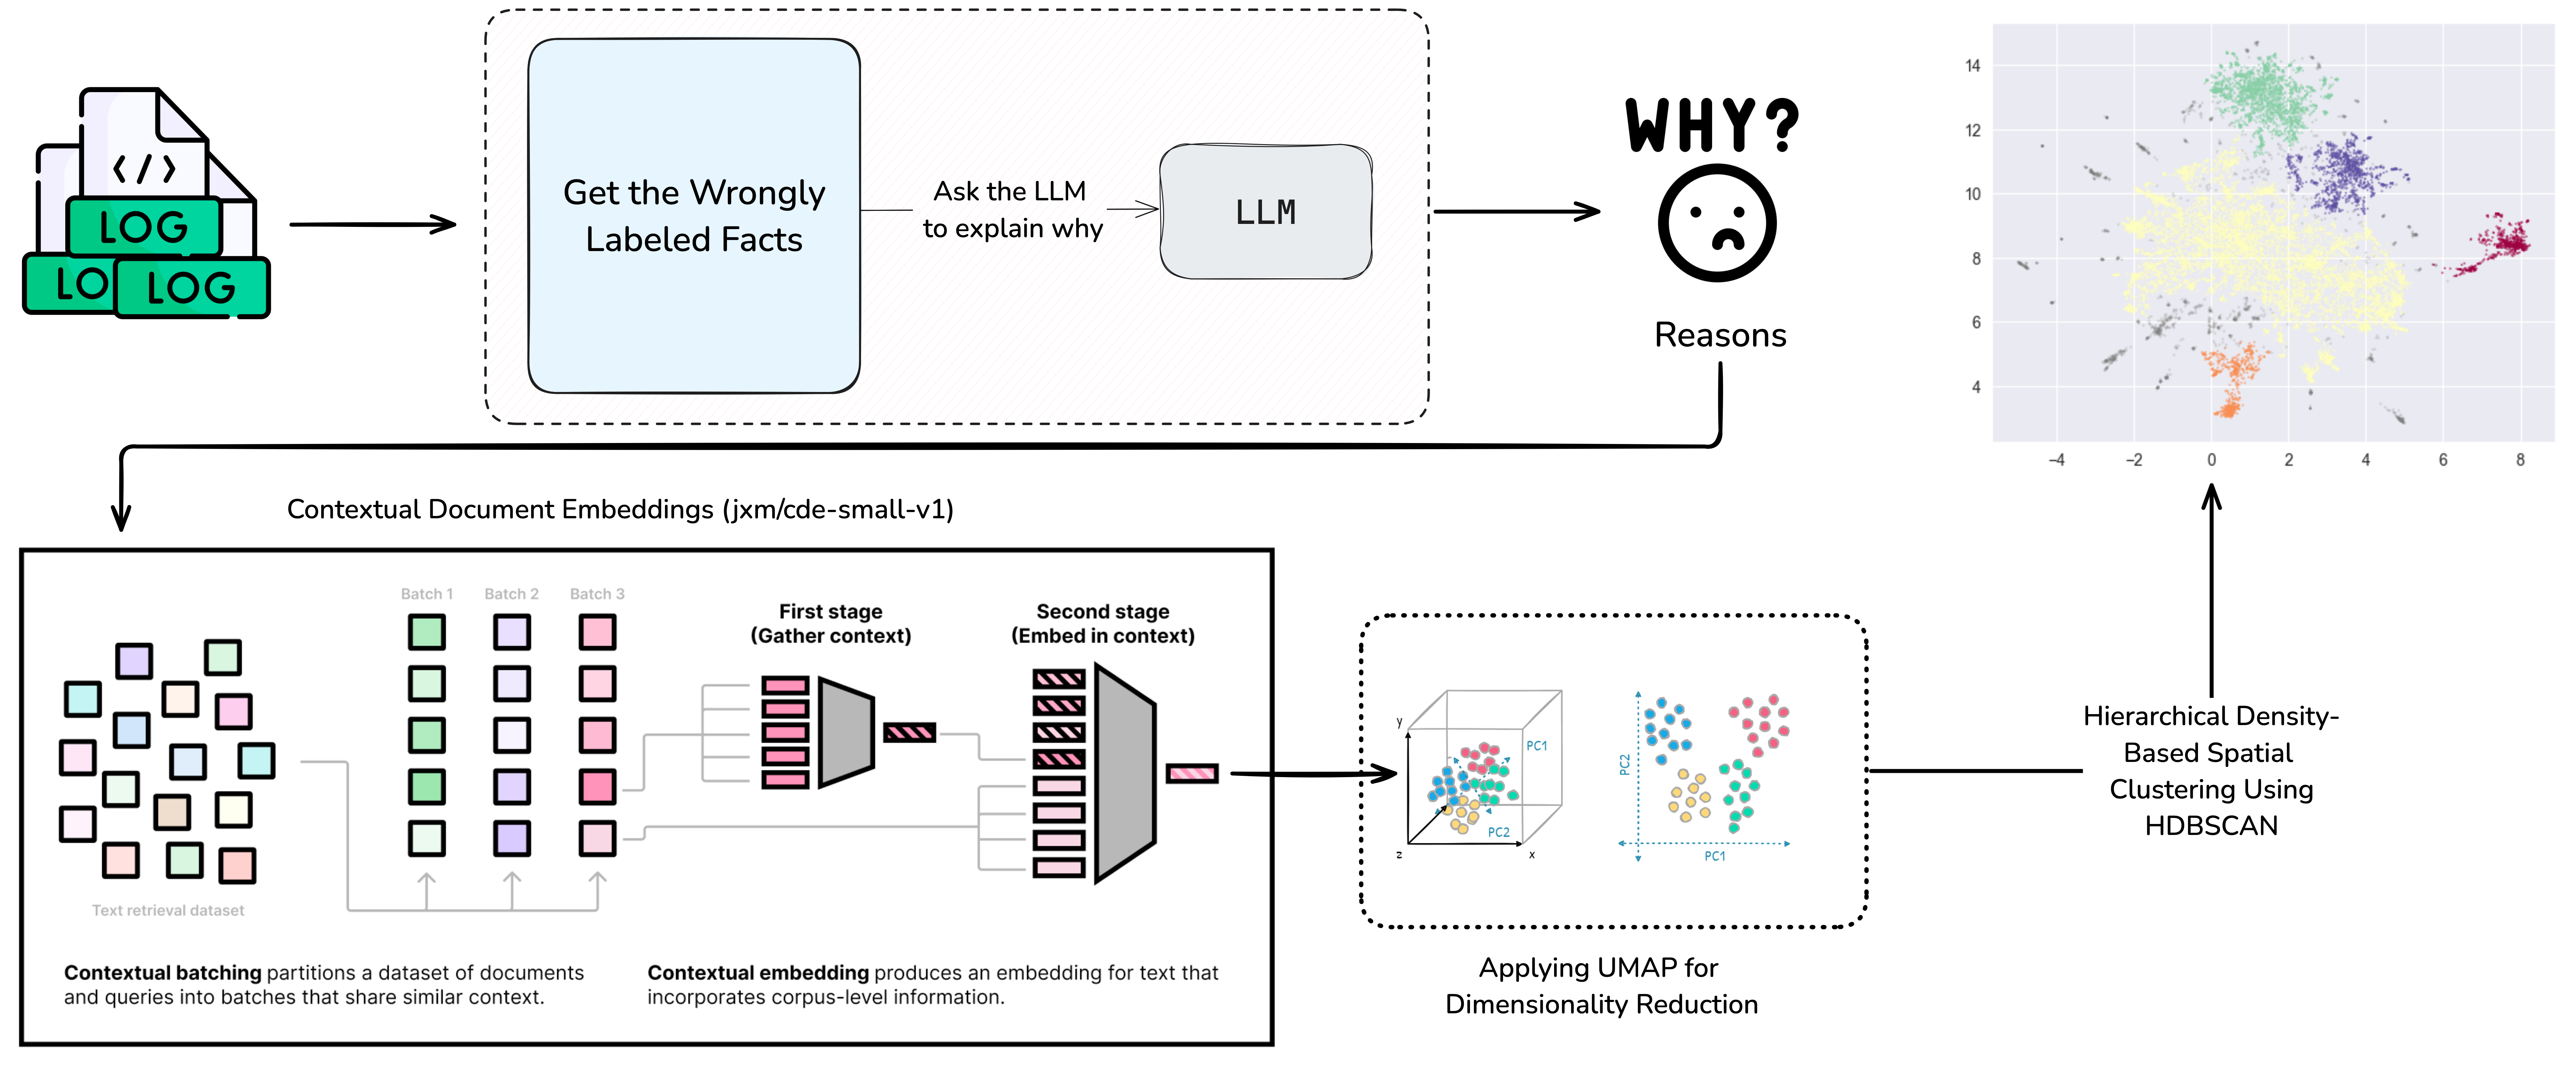
\includegraphics[width=\textwidth]{res/clustering}
    \end{minipage}
    \caption{Collecting logs and leveraging LLM-generated reasoning, combined with contextual document embeddings (jxm/cde-small-v1)~\cite{morris2024contextualdocumentembeddings}, to cluster errors using a hierarchical density-based spatial technique.}
    \label{fig:error-clustering-task}
\end{figure}

As depicted in Figure~\ref{fig:error-clustering-task}, our objective is to categorize errors by LLMs and text embedding model.
This approach helps reveal common error types and patterns by clustering explanations into distinct groups.
The process begins by gathering logs of incorrectly labeled data, referred to here as "wrongly labeled facts."
These logs are analyzed, and we then prompt an LLM to generate explanations, or "reasons," for each error.
This step provides context and may highlight underlying patterns or causes that contribute to these errors.
The prompt template used for this reasoning process is detailed in Appendix~\ref{sec:prompt-templates:reasoning}.
After obtaining explanations from the LLM, we use a specialized text embedding model named "jxm/cde-small-v1"~\footnote{\url{https://huggingface.co/jxm/cde-small-v1}}.
We selected cde-small-v1 because it is the highest-ranked small model (under 400 million parameters) on the MTEB leaderboard for text embedding models, as of October 1, 2024.
This model transforms each explanation into a contextualized embedding, capturing both semantic meaning and specific instruction-driven nuances for each error's context~\cite{morris2024contextualdocumentembeddings}.
Next, these embeddings undergo dimensionality reduction using Uniform Manifold Approximation and Projection (UMAP), a technique that projects high-dimensional data into two or three dimensions while preserving local and some global structure.
UMAP's visualization helps identify potential clusters or groupings of similar errors, making it easier to observe patterns that might be difficult to see in higher dimensions.
Once reduced in dimensionality, the embeddings are fed into Hierarchical Density-Based Spatial Clustering of Applications with Noise (HDBSCAN), a clustering algorithm well-suited for discovering clusters in data with varying density.
HDBSCAN clusters the error embeddings based on their density, identifying groups of similar errors and isolating outliers.
Following clustering, we identify some reasons from each dataset.
These representative reasons are then provided to an LLM to assign descriptive labels to each error category, which encapsulate the main types of errors across the dataset.

The labeling data for each cluster is as follows:
\begin{itemize}
    \item \textbf{UnLabeled:} The information or context provided does not contain the claimed details, such as references to specific individuals, places, or events that are purportedly associated with the topic.
    \item \textbf{Relationship Errors:} Errors arise from misstatements regarding relationships between people, such as marital status or religious affiliations that conflict with the provided details.
    \item \textbf{Role Attribution Errors:} Errors are due to incorrect associations of individuals with particular roles, places, or teams that do not match the details in the context.
    \item \textbf{Geographic/Nationality Errors:} This category includes errors related to locations, national affiliations, or settings that do not align with the context or provide contradictory information.
    \item \textbf{Genre/Classification Errors:} Misclassifications of films, genres, or roles are highlighted here, especially when certain works are wrongly associated with people, studios, or genres.
    \item \textbf{Identifier/Biographical Errors:} These errors involve incorrect identifiers or biographical details, such as award titles, label names, or authorship that don’t match the context.
\end{itemize}


\begin{table}[ht!]
    \noindent
    \caption{Dataset-wise error clustering based on LLM-generated reasoning, using Contextual Document Embeddings for embeddings, UMAP, and HDBSCAN.}
    \resizebox{\textwidth}{!}{
    \begin{threeparttable}
        \begin{tabular}{llcccccc||c}
            \toprule
            \textbf{Dataset}            & \textbf{Model} & \textbf{UnLabeled} & \textbf{Relationship} & \textbf{Role Errors} & \textbf{Geo Errors} & \textbf{Classification} & \textbf{Identifiers} & \textbf{Total}\tnote{*} \\
            \midrule
            \multirow{5}{*}{FactBench}  & Gemma2                             & 4    & 36    & 45    & 176  & 13     & 1     & 275 \\
                                        & Qwen2.5                            & 33   & 27    & 60    & 194  & 34     & 1     & 349 \\
                                        & Llama3.1                           & 38   & 44    & 73    & 295  & 38     & 3     & 491 \\
                                        & Mistral                            & 53   & 27    & 53    & 242  & 40     & 2     & 417 \\ \cline{2-9}
                                        & Unique. Ratio (\%)                 & 0.62 & 0.72  & 0.44  & 0.52 & 0.63   & 0.57  & 0.53 \\ \hline
            \multirow{5}{*}{YAGO}       & Gemma2                             & 6        & 134   & 0   & 14      & 51    & 2     & 207   \\
                                        & Qwen2.5                            & 7        & 109   & 0   & 13      & 63    & 2     & 194   \\
                                        & Llama3.1                           & 8        & 98    & 0   & 19      & 104   & 2     & 231   \\
                                        & Mistral                            & 7        & 54    & 0   & 10      & 34    & 3     & 108   \\ \cline{2-9}
                                        & Unique. Ratio (\%)                 & 0.35     & 0.52  & --   & 0.46    & 0.51  & 0.33  & 0.50  \\ \hline
            \multirow{5}{*}{DBpedia}    & Gemma2                             & 353      & 22    & 98  & 1729    & 459   & 299   & 2960  \\
                                        & Qwen2.5                            & 339      & 19    & 91  & 1525    & 357   & 237   & 2568 \\
                                        & Llama3.1                           & 382      & 28    & 109 & 2172    & 509   & 318   & 3518 \\
                                        & Mistral                            & 325      & 20    & 94  & 1487    & 438   & 241   & 2605 \\ \cline{2-9}
                                        & Unique. Ratio (\%)                 & 0.41     & 0.43  & 0.44 & 0.42   & 0.42  & 0.40  & 0.41 \\
            \bottomrule
        \end{tabular}
    \begin{tablenotes}
         \item[*] Some errors may not be included in this analysis because we did not receive any responses for them. While we classify these as incorrect predictions, they are not considered in the error analysis section.
    \end{tablenotes}
    \end{threeparttable}}
    \label{tab:error_results-full-wo-category-all-datasets}
\end{table}

\begin{figure}[ht!]
    \centering
    \begin{minipage}[b]{\textwidth}
        \centering
        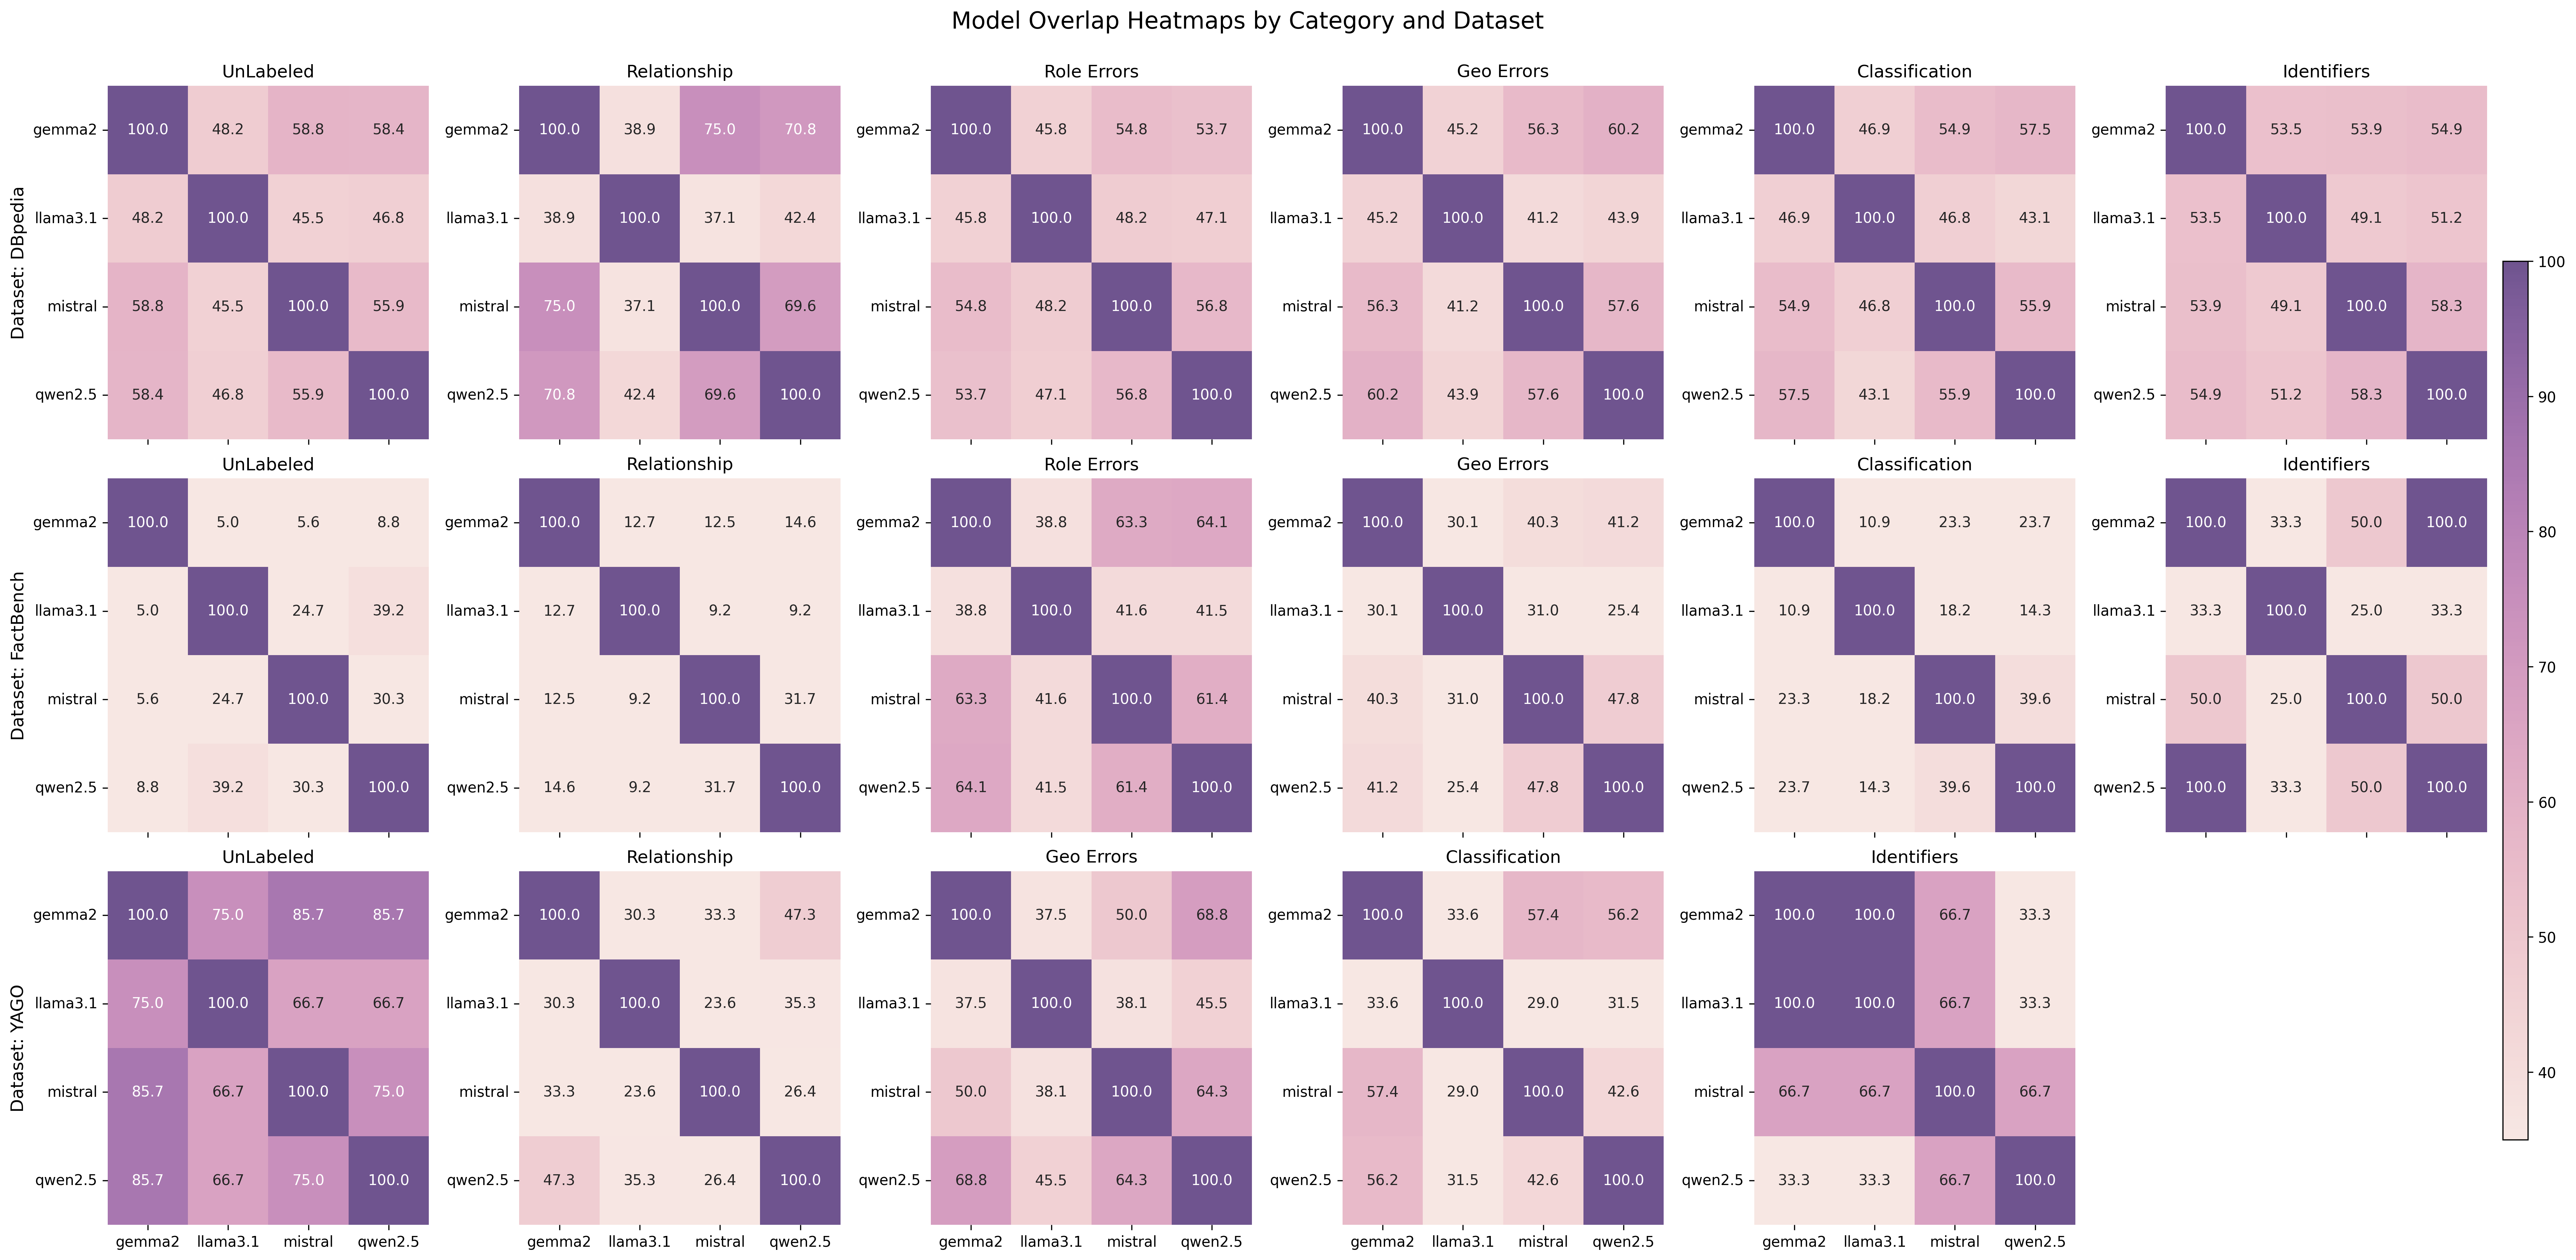
\includegraphics[width=\textwidth]{res/overlap_heatmaps_by_dataset}
    \end{minipage}
    \caption{Model overlap heatmaps by category and dataset. Each cell shows the percentage overlap in errors between model pairs. Matrices are organized by error category (UnLabeled, Relationship, Role Errors, etc.) and dataset (DBpedia, FactBench, YAGO), revealing patterns in how models agree or disagree when making verification errors.}
    \label{fig:overlap_heatmaps_by_dataset}
\end{figure}

The heatmaps in Figure~\ref{fig:overlap_heatmaps_by_dataset} visualize the overlap in error patterns between different models across error categories and datasets.
The overlap matrices reveal distinct patterns of agreement and disagreement between models when making errors, with darker colors indicating higher overlap percentages.
For \textit{DBpedia}, we observe moderate to high overlap (45-75\%) between models across most error categories, suggesting similar challenges in handling complex factual relationships.
The \textit{FactBench} dataset shows lower overlap percentages (30-40\% typical), indicating more independent error patterns between models.
\textit{YAGO} exhibits variable overlap, with particularly high agreement in unlabeled errors (75-85\% overlap) but lower overlap in relationship errors (23-35\%).
These patterns suggest that while models often struggle with similar types of facts, they also make distinct errors, supporting the value of ensemble approaches.
The lower overlap in \textit{FactBench} errors particularly validates our multi-model verification strategy.

\begin{figure}[ht!]
    \centering
    \begin{minipage}[b]{0.42\textwidth}
        \centering
        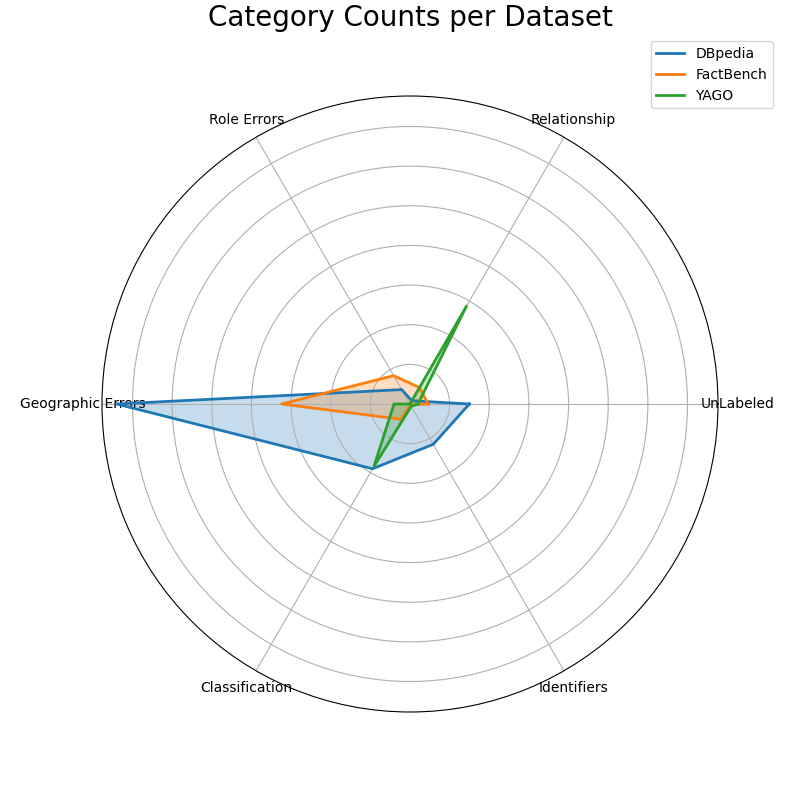
\includegraphics[width=\textwidth]{res/radarChart-normalized}
        \caption{Normalized distribution of error clusters across datasets.}
        \label{fig:normalized_distribution_of_error_clusters}
    \end{minipage}
    \hspace{0.05\textwidth} % Space between the images
    \begin{minipage}[b]{0.42\textwidth}
        \centering
        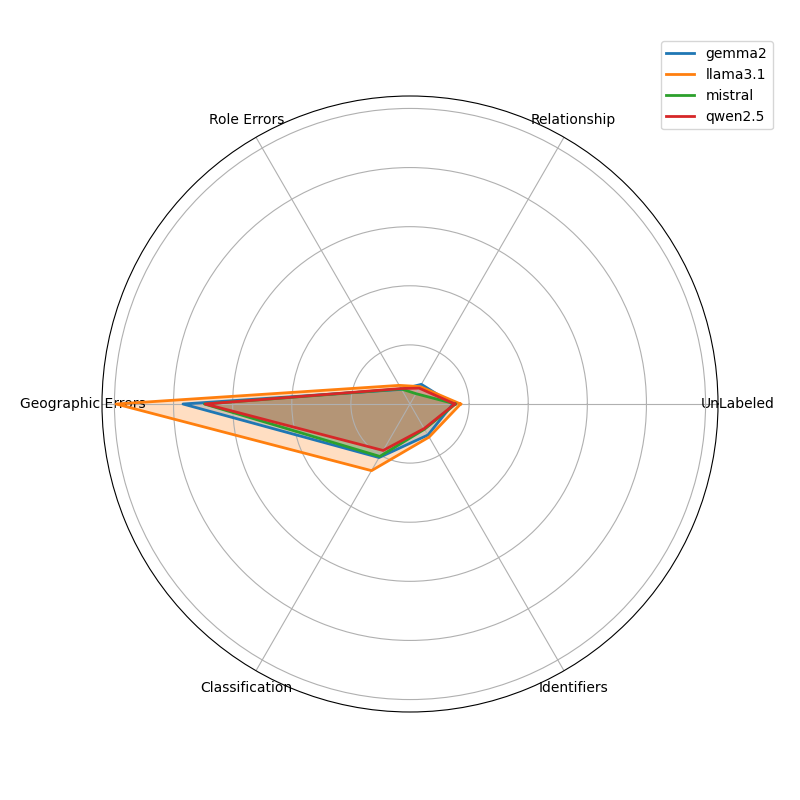
\includegraphics[width=\textwidth]{res/radarChart-normalized-llms}
        \caption{Distribution of error clusters across selected LLMs.}
        \label{fig:distribution_of_error_clusters}
    \end{minipage}
\end{figure}

\begin{figure}[ht!]
    \centering
    \begin{minipage}[b]{0.42\textwidth}
        \centering
        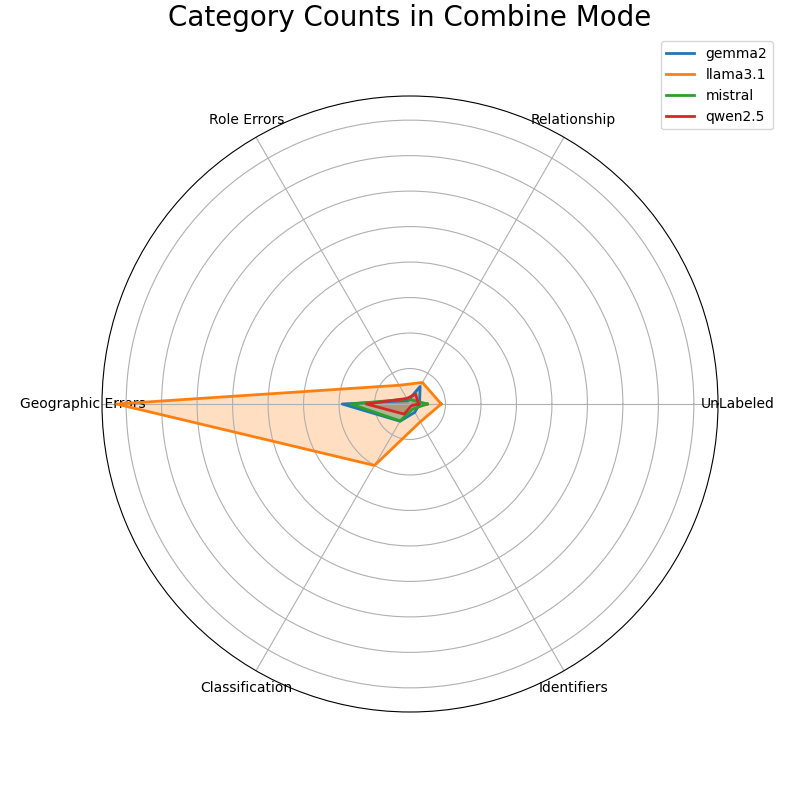
\includegraphics[width=\textwidth]{res/radarChart-normalized-llms-1}
    \end{minipage}
    \hspace{0.05\textwidth} % Space between the images
    \begin{minipage}[b]{0.42\textwidth}
        \centering
        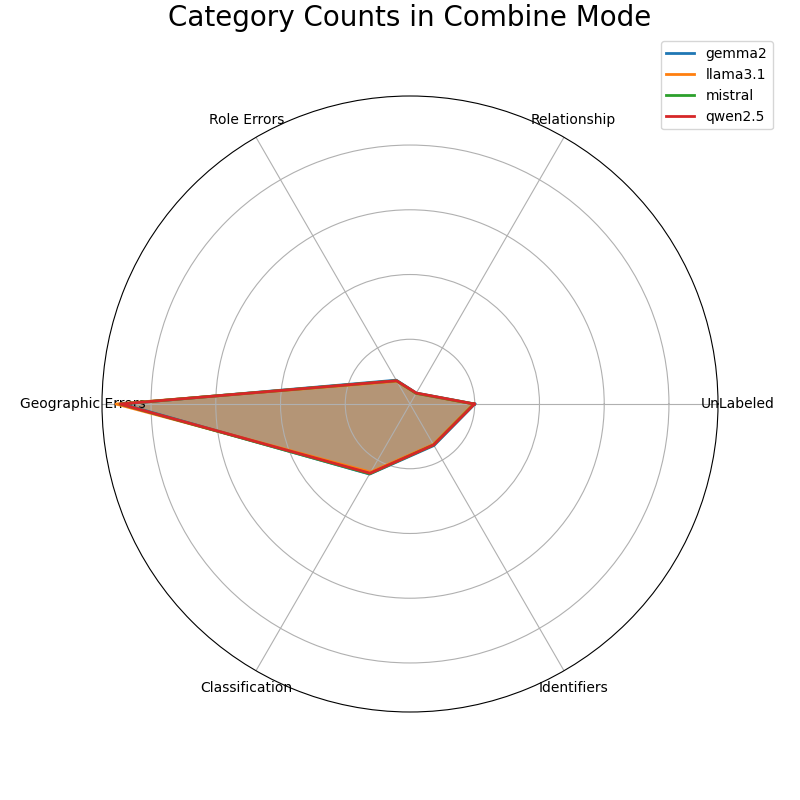
\includegraphics[width=\textwidth]{res/radarChart-normalized-llms-4}
    \end{minipage}
    \caption{Distribution of tendency to be wrong across gemma2, qwen2.5, LLama3.1 and mistral models. The right chart illustrates the distribution of fully incorrect predictions (4/4) detailing the instances where all predictions made by the models were incorrect. The left chart depicts the distribution of just one wrong predictions (1/4).}
    \label{fig:distribution_of_error_clusters_1_4}
\end{figure}

Results from Table~\ref{tab:error_results-full-wo-category-all-datasets} alongside Figures~\ref{fig:normalized_distribution_of_error_clusters}, ~\ref{fig:distribution_of_error_clusters}, and~\ref{fig:distribution_of_error_clusters_1_4} highlight both common challenges and model-specific characteristics in fact validation performance.

Geographic and nationality-related errors emerged as the predominant challenge, accounting for 56.9\% of total errors across all models and datasets.
This pattern was particularly pronounced in the \textit{DBpedia} dataset, where geographic errors constituted 58.5\% of all errors, suggesting a systematic challenge in processing and validating location-based information.
This pervasive difficulty across all models indicates a fundamental challenge in handling geographic relationships and facts.

The analysis of dataset-specific patterns revealed distinct characteristics and challenges.
The \textit{DBpedia} dataset proved to be the most challenging, generating the highest error count and showing particular vulnerability to geographic and classification errors.
In contrast, the \textit{FactBench} dataset demonstrated a more balanced distribution of errors across categories, though still showing a predominance of geographic errors.
The \textit{YAGO} dataset exhibited a unique pattern, with relationship errors being the most frequent, followed by classification errors, and notably showing no role attribution errors a distinctive characteristic that sets it apart from other datasets.

When examining model-specific performance, \textit{LLama3.1} consistently generated the highest error counts across datasets, showing particular vulnerability to geographic errors in the \textit{DBpedia} dataset and elevated classification errors compared to other models.
\textit{Mistral}, on the other hand, demonstrated stronger overall performance, particularly in the \textit{YAGO} dataset.
\textit{Gemma2} and \textit{Qwen2.5} showed similar error patterns and counts, positioning themselves between \textit{LLama3.1} and \textit{Mistral} in terms of performance.

The hierarchical distribution of error types shows a consistent pattern across models.
This consistency in error distribution suggests that these challenges are inherent to the task rather than model-specific limitations.

Despite varying error counts, models maintained similar error distribution patterns within each dataset, indicating that these challenges are systematic rather than model-specific.
The analysis suggests several critical areas for future development in LLM fact validation capabilities.
Primary attention should be directed toward enhancing geographic and location-based reasoning capabilities, given their dominant role in error generation.
Additionally, improving classification tasks and the handling of insufficient context or ambiguous information could significantly enhance overall performance.
The consistent patterns across models suggest that these improvements would benefit the field broadly rather than being model-specific enhancements.

\subsection{DBpedia Analysis in Depth}\label{subsec:db}
Since \textit{DBpedia} proved to be the most challenging dataset in our evaluation, we performed a deeper analysis based on the dataset stratification established by Marchesin et al.~\cite{Marchesin_Silvello_Alonso_2024}.
Each knowledge graph triple was assigned to one of seven partitions, numbered 1--7, where partition 1 represents the least popular/common knowledge and partition 7 represents the most popular/common knowledge.
This stratification helps us understand how our verification system performs across different levels of fact popularity and complexity within \textit{DBpedia}.
The analysis can reveal whether the system's accuracy varies between common, well-documented facts versus more obscure or specialized knowledge.
This insight is valuable for identifying areas where the system needs improvement and understanding its real-world applicability across different types of knowledge.

\begin{table}[ht!]
    \noindent
    \caption{Partition-wise evaluation results of the proposed system and candidate LLMs over the DBpedia dataset.}
    \resizebox{\textwidth}{!}{
        \begin{tabular}{lcccccccccccccccc}
            \toprule
            & \multirow{2}{*}{\textbf{Weight}} & \multirow{2}{*}{\textbf{Size}} & \multicolumn{2}{c}{\textbf{Gemma2}}       & \multicolumn{2}{c}{\textbf{Qwen2.5}}          & \multicolumn{2}{c}{\textbf{Llama3.1}}         & \multicolumn{2}{c}{\textbf{Mistral}}     & \multicolumn{2}{c}{\textbf{Qwen2.5:14b}}         & \multicolumn{2}{c}{\textbf{Llama3.1:70b}} \\ \cmidrule(lr){4-5} \cmidrule(lr){6-7} \cmidrule(lr){8-9} \cmidrule(lr){10-11} \cmidrule(lr){12-13} \cmidrule(lr){14-15}
            & & & \textbf{Acc}         & \textbf{F1}       & \textbf{Acc}          & \textbf{F1}           & \textbf{Acc}            & \textbf{F1}         & \textbf{Acc}             & \textbf{F1}     & \textbf{Acc}               & \textbf{F1}         & \textbf{Acc}                & \textbf{F1} \\
            \midrule
            Stratum 1    &  0.9120   & 2223 & 0.672                & 0.773             & 0.708                 & 0.804                 & 0.600                   & 0.712               & 0.710                   & 0.806          & 0.688                      & 0.786               & 0.700                       & 0.797       \\
            Stratum 2    &  0.0616   & 1695 & 0.697                & 0.796             & 0.720                 & 0.816                 & 0.627                   & 0.738               & 0.726                   & 0.820          & 0.711                      & 0.807               & 0.720                       & 0.814       \\
            Stratum 3    &  0.0177   & 1588 & 0.689                & 0.791             & 0.736                 & 0.828                 & 0.632                   & 0.743               & 0.719                   & 0.819          & 0.708                      & 0.806               & 0.719                       & 0.815       \\
            Stratum 4    &  0.0044   & 1327 & 0.689                & 0.797             & 0.737                 & 0.835                 & 0.628                   & 0.747               & 0.709                   & 0.815          & 0.706                      & 0.811               & 0.714                       & 0.817       \\
            Stratum 5    &  0.0029   & 1058 & 0.666                & 0.780             & 0.705                 & 0.813                 & 0.638                   & 0.758               & 0.724                   & 0.826          & 0.690                      & 0.800               & 0.695                       & 0.804       \\
            Stratum 6    &  0.0010   & 814  & 0.692                & 0.800             & 0.719                 & 0.822                 & 0.614                   & 0.739               & 0.733                   & 0.833          & 0.709                      & 0.813               & 0.708                       & 0.812       \\
            Stratum 7    &  0.0001   & 629  & 0.671                & 0.776             & 0.779                 & 0.864                 & 0.650                   & 0.762               & 0.754                   & 0.848          & 0.731                      & 0.826               & 0.747                       & 0.838       \\
            \bottomrule
        \end{tabular}}
    \label{tab:evaluation_results-partition-wise-dbpedia}
\end{table}

The weights declared in Table~\ref{tab:evaluation_results-partition-wise-dbpedia} are gathered by Marchesin et al.~\cite{Marchesin_Silvello_Alonso_2024}, stratum 1 contains the vast majority of the triplets in DBpedia.
This makes sense because stratum 1 represents the lowest-utility facts - those that are rarely used in queries.

\begin{figure}[ht!]
    \centering
    \begin{minipage}[b]{\textwidth}
        \centering
        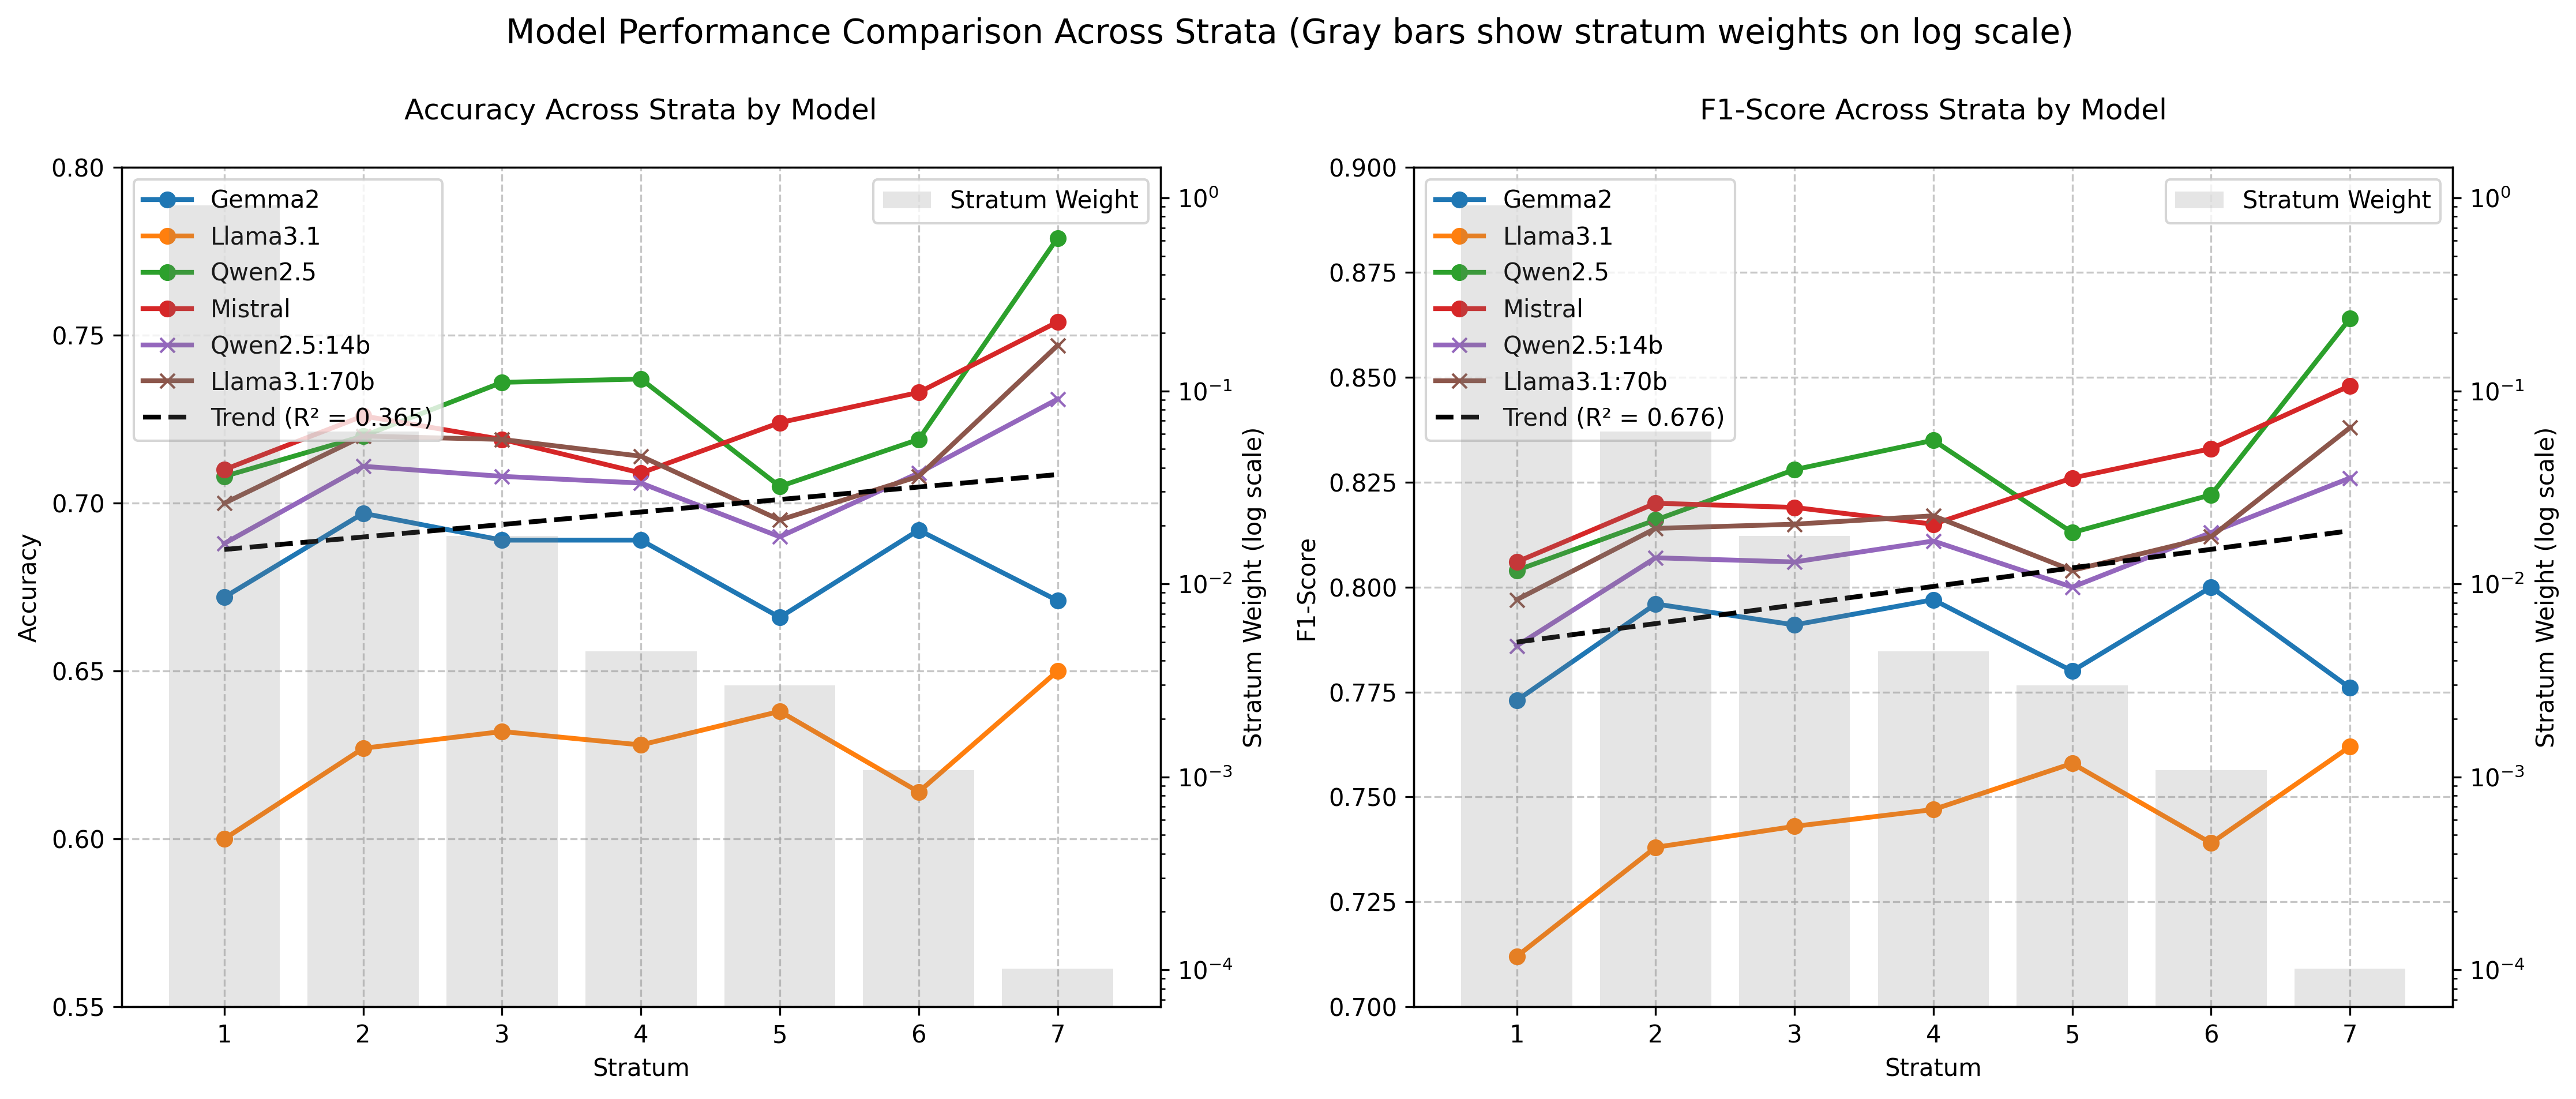
\includegraphics[width=\textwidth]{res/F1_ACC_Analysis_Across_Stratum}
    \end{minipage}
    \caption{Partition-wise model performance comparison: Accuracy and F1-scores for knowledge graph fact verification on DBpedia dataset. Gray bars indicate stratum weights (log scale).}
    \label{fig:F1_ACC_Analysis_Across_Stratum}
\end{figure}

Table~\ref{tab:evaluation_results-partition-wise-dbpedia} and Figure~\ref{fig:F1_ACC_Analysis_Across_Stratum}, demonstrate that the models have a clear trend of improved performance on more common knowledge.
\textit{Qwen2.5} exhibits particularly strong performance, with accuracy increasing from 0.708 in Stratum 1 to 0.779 in Stratum 7, and F1-scores following a similar upward trajectory.
This suggests that the model benefits from the richer context and more consistent representation of popular facts in the knowledge base.

The performance disparity between lower and higher strata highlights a common challenge in knowledge graph verification: the system's reliability varies with fact popularity.
This insight is particularly valuable for real-world applications, where handling both common and specialized knowledge is crucial.

Building on our previous analysis of \textit{DBpedia} results, we conducted a stratum-wise error analysis to better understand how error distributions vary across different data partitions.
Our analysis of error patterns across knowledge strata showed in Figure~\ref{fig:error_model-comparison_partition-wise} declares distinct performance characteristics among the four LLMs.
The models demonstrated varying levels of effectiveness in handling knowledge from different popularity strata, with error rates showing notable patterns across the commonality spectrum.

\begin{figure}[ht!]
    \centering
    \begin{minipage}[b]{\textwidth}
        \centering
        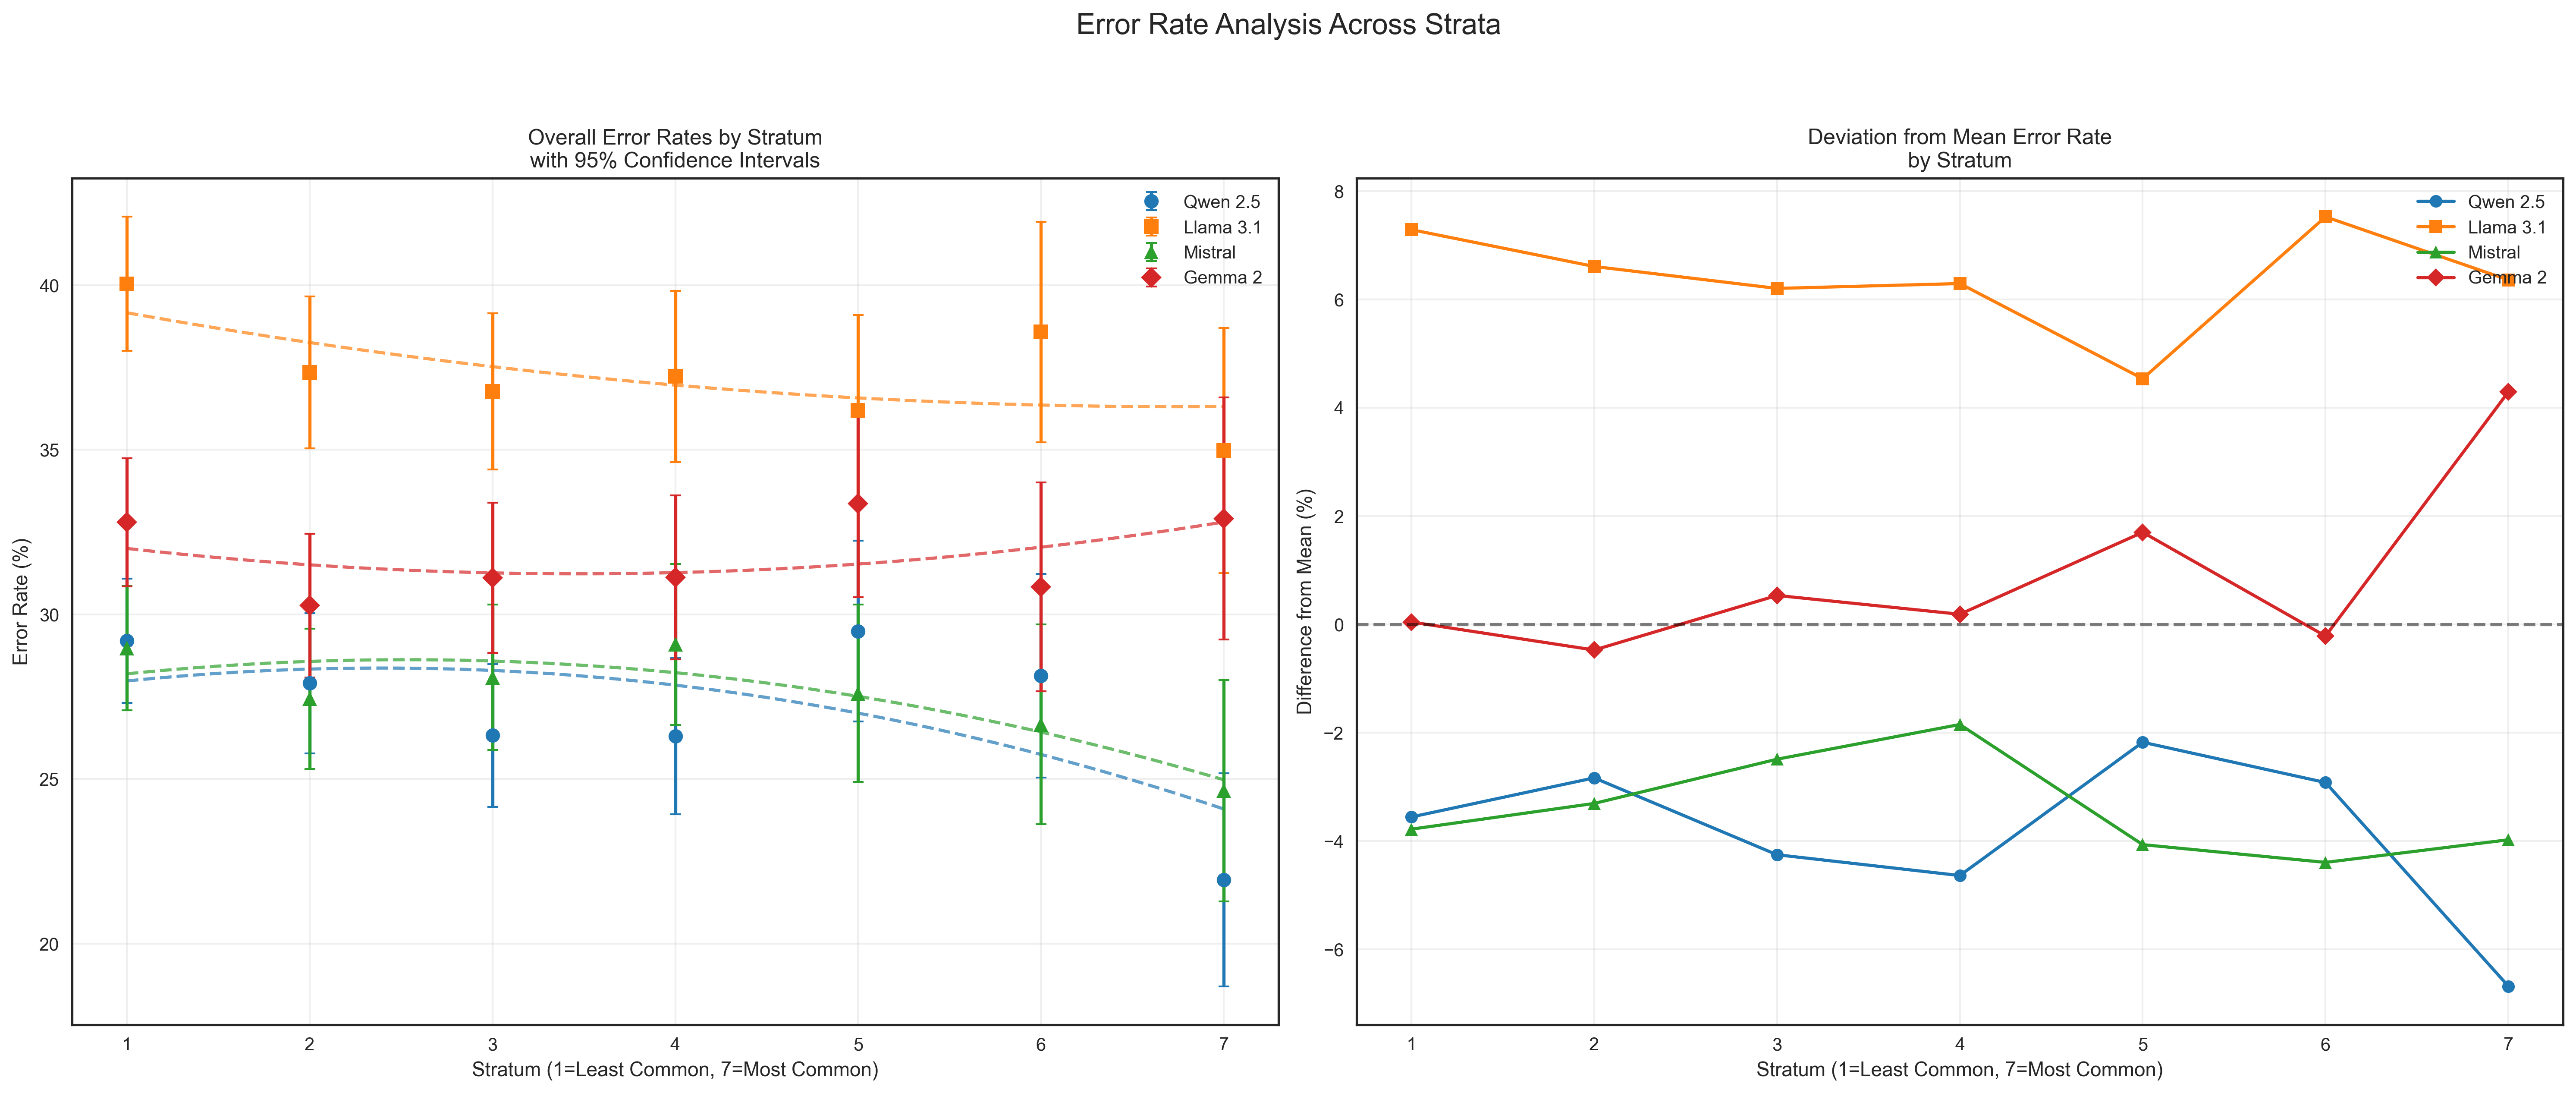
\includegraphics[width=\textwidth]{res/error_rates_analysis}
    \end{minipage}
    \caption{Error distribution analysis across different language models and frequency strata.}
    \label{fig:error_model-comparison_partition-wise}
\end{figure}

\textit{Llama3.1} exhibited the highest overall error rate (37.31\% ± 1.51\%), significantly exceeding other models' error rates.
Despite its higher error rate, \textit{Llama3.1} maintained relatively consistent performance across strata (range: 34.98\% - 40.04\%), suggesting uniform handling of both common and rare knowledge.
The model showed a slight negative correlation with stratum number (r=-0.628, p=0.1309), indicating a modest tendency to perform better with more common knowledge, though this trend was not statistically significant.

In contrast, \textit{Qwen2.5} and \textit{Mistral} demonstrated notably lower error rates (27.04\% ± 2.38\% and 27.50\% ± 1.41\% respectively), with \textit{Mistral} showing the most pronounced negative correlation with stratum number (r=-0.761, p=0.0470).
This statistically significant correlation indicates that \textit{Mistral's} performance improves substantially as knowledge becomes more common.
\textit{Qwen2.5} showed the widest range of error rates (21.94\% - 29.49\%), suggesting more variable performance across different knowledge types.

\textit{Gemma2} maintained an intermediate position with a mean error rate of 31.77\% ± 1.13\% and showed the most stable performance across strata (range: 30.27\% - 33.36\%).
Uniquely among the models, \textit{Gemma2} exhibited a slight positive correlation with stratum number (r=0.237, p=0.6083), though this trend was not statistically significant.
In general, it has the most uniform error distribution across strata.

\begin{figure}[ht!]
    \centering
    \begin{minipage}[b]{\textwidth}
        \centering
        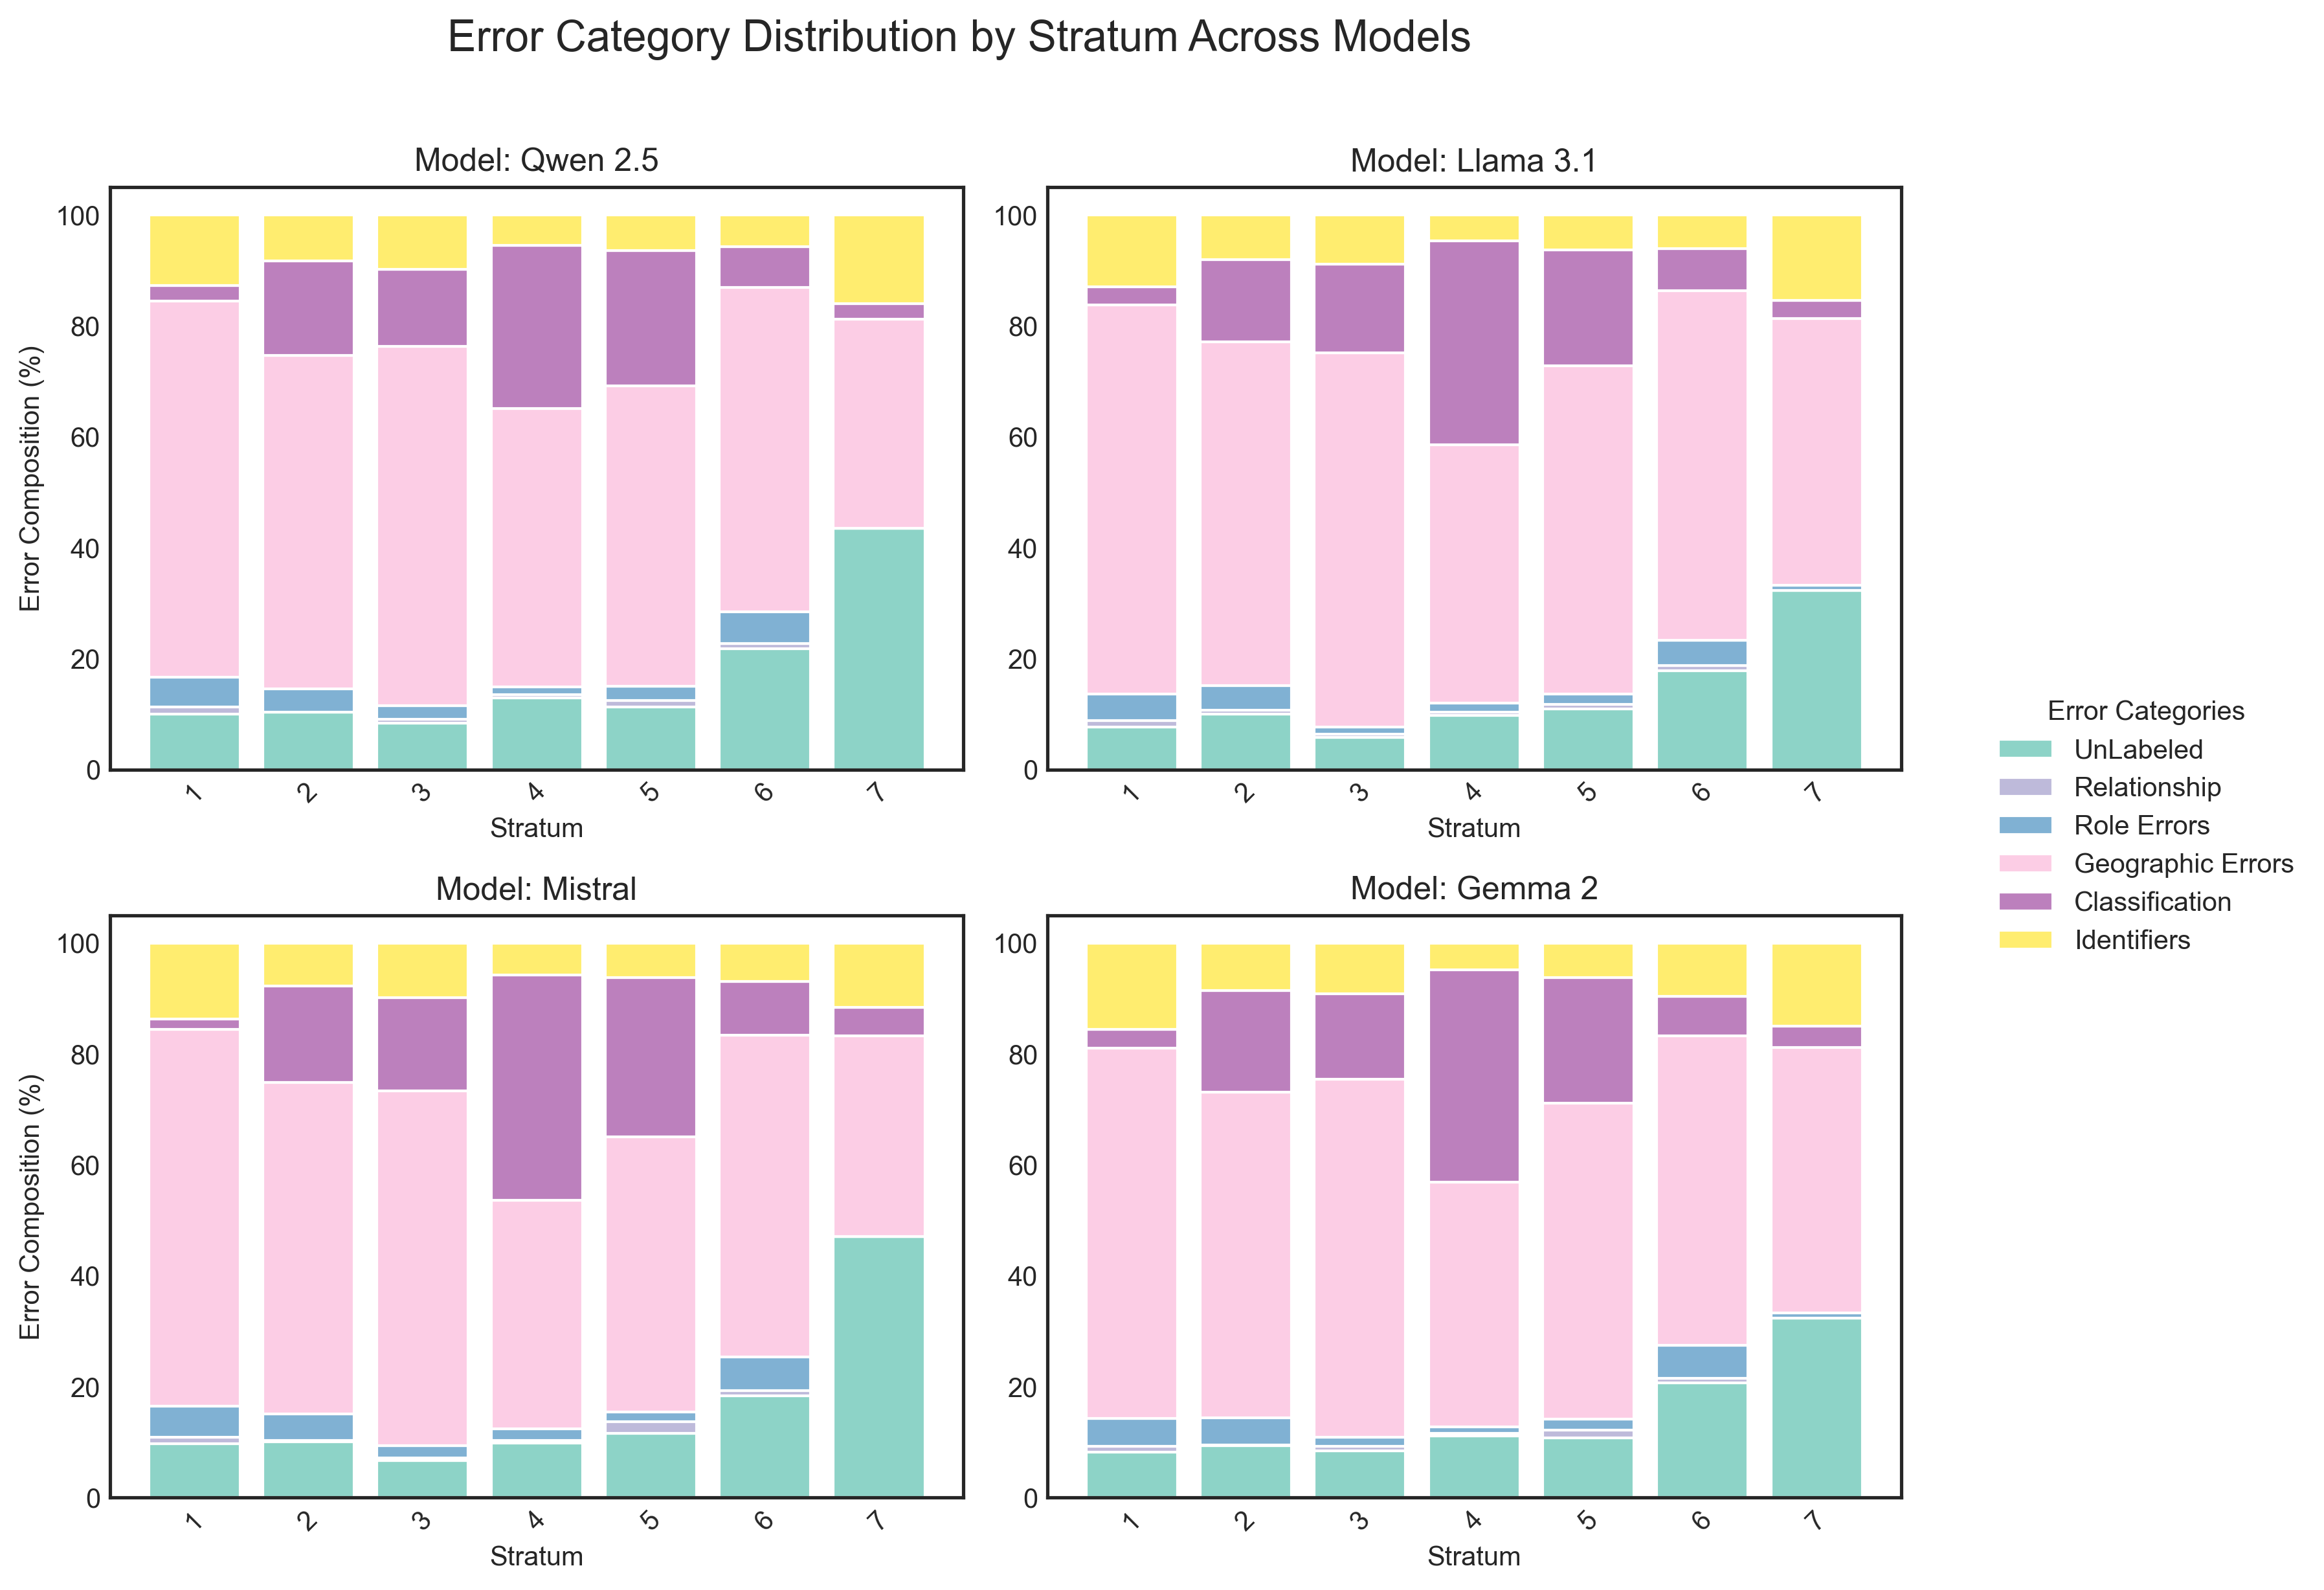
\includegraphics[width=\textwidth]{res/category_distribution_analysis}
    \end{minipage}
    \caption{distribution of error categories across different language models and frequency strata}
    \label{fig:category_distribution_analysis}
\end{figure}

Analysis of error categories in Figure~\ref{fig:category_distribution_analysis} reported separate patterns across strata, with certain error types becoming more prevalent in specific knowledge domains.
The proportion of unLabeled errors increased notably in the most common knowledge strata (6-7), while geographic errors showed higher prevalence in less common knowledge strata (1-3).
Classification errors maintained relatively consistent proportions across all strata, suggesting that this type of error is less influenced by knowledge commonality.

These findings suggest that while newer models like \textit{Qwen2.5} achieve lower overall error rates, they may be more sensitive to knowledge popularity, performing notably better with common knowledge.
In contrast, models like \textit{Gemma2} offer more consistent performance across knowledge types, potentially making them more reliable for applications requiring uniform handling of both common and rare knowledge.

\begin{figure}[ht!]
    \centering
    \begin{minipage}[b]{\textwidth}
        \centering
        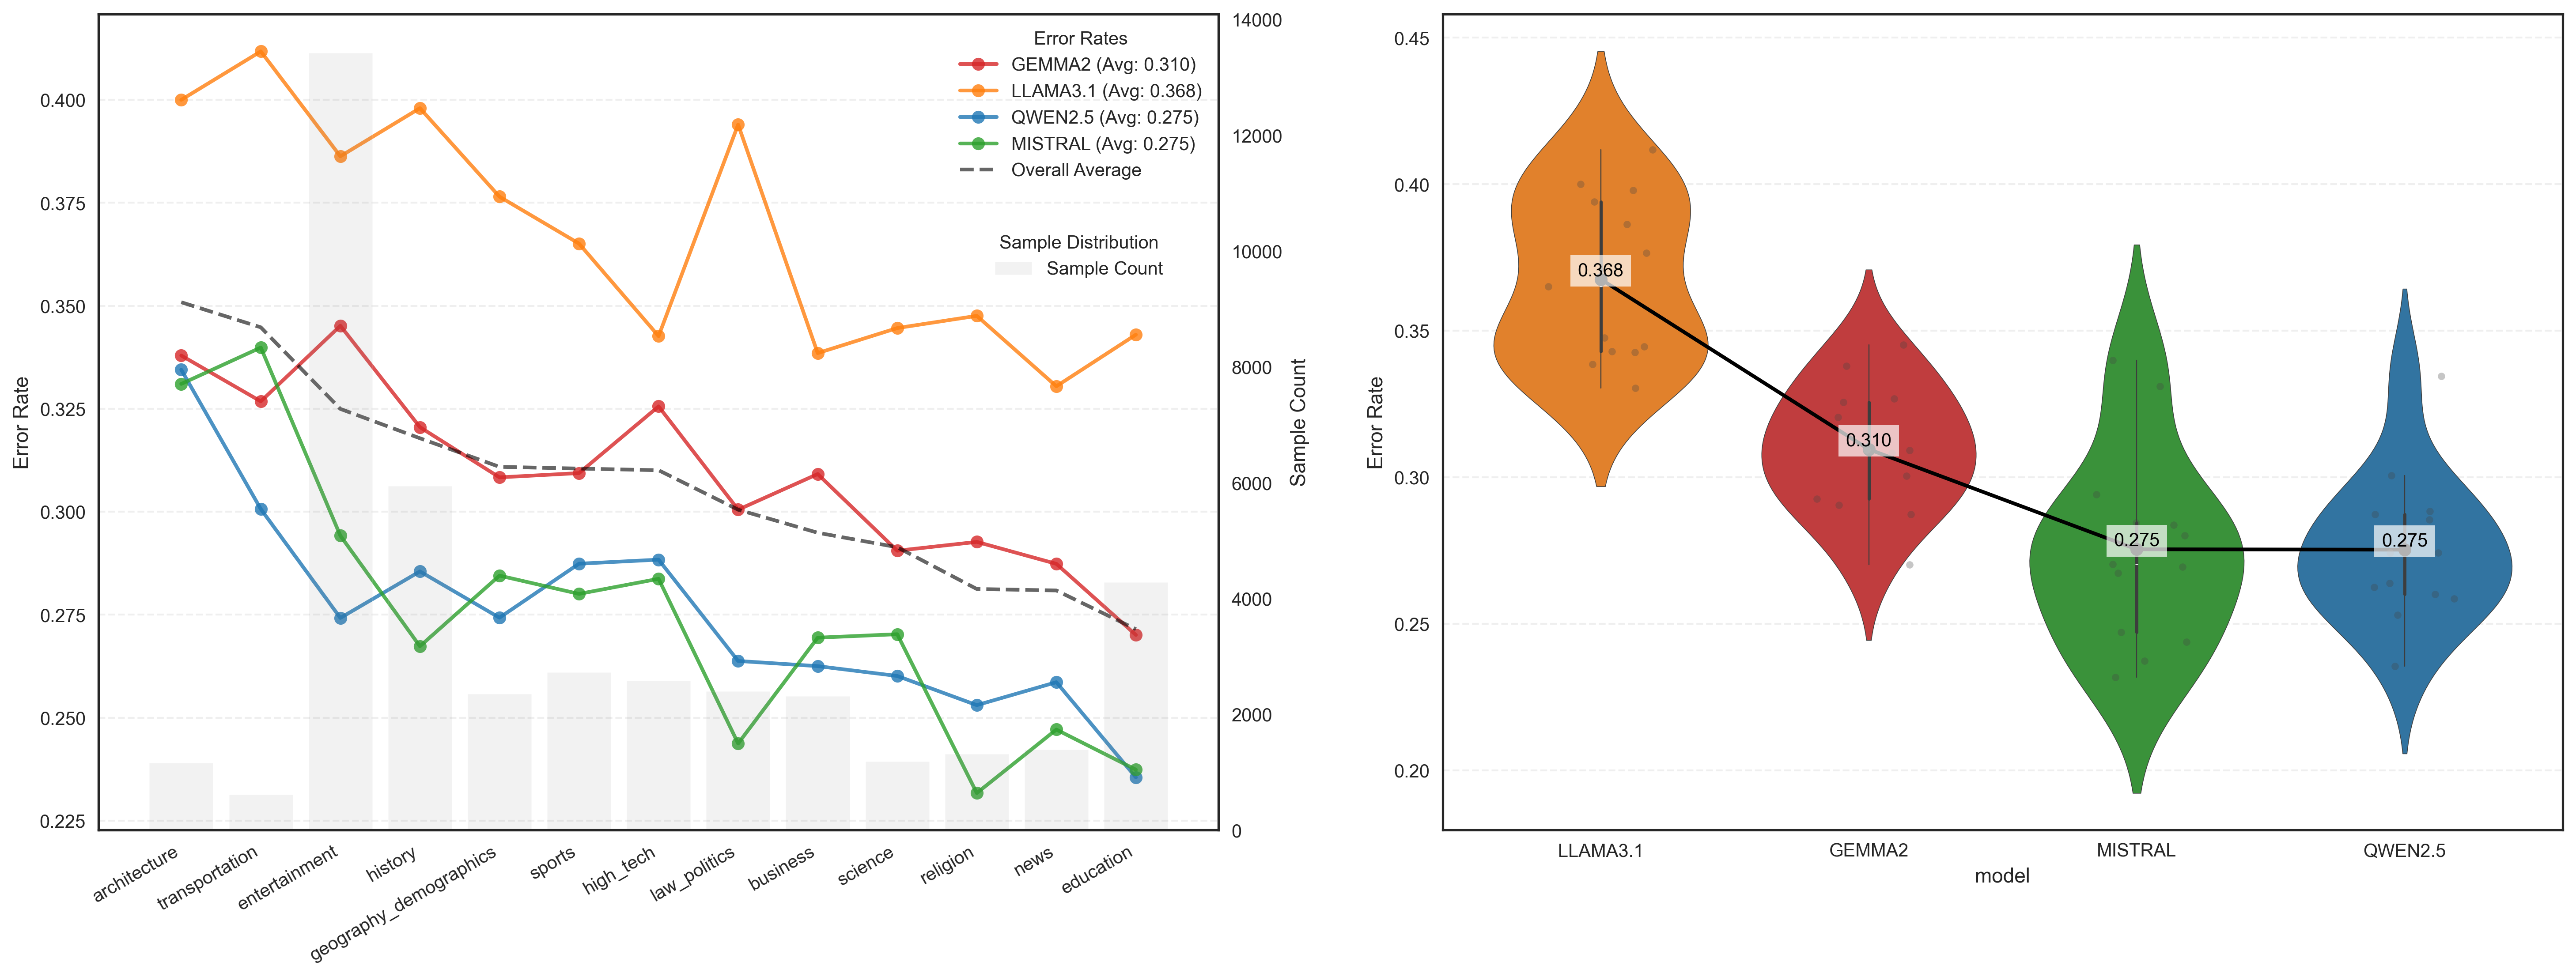
\includegraphics[width=\textwidth]{res/combined-model-analysis}
    \end{minipage}
    \caption{Comparative analysis of language model error rates across knowledge domains. (Left) domain-specific error ratesacross 13 knowledge categories, with overlaid sample distribution bars. (Right) distribution of error rates for each model}
    \label{fig:topic_distribution_analysis}
\end{figure}

By employing BERTopic from the work of Marchesin et al.~\cite{Marchesin_Silvello_Alonso_2024} to generate interpretable clusters, we obtained 64 distinct clusters, which were manually scrutinized and aggregated to form a set of 13 broad topics.
These topics encompass “Architecture", "Business", "Education", "Entertainment", "Geography", "High Tech", "History", "Law and Politics", "News", "Religion", "Science", "Sports", and  "Transportation".
Some facts were not assigned to any topic or were assigned to multiple topics.

As showed in Figure~\ref{fig:topic_distribution_analysis} "Education" and "News" domains consistently show lower error rates across all models.
"Architecture" and "Transportation" categories present higher error rates, particularly for \textit{Llama3.1}.
High variance is observed in the "Business" and "Law and Politics" domains, suggesting these may be more challenging areas for current models.
Also we figured out that \textit{Qwen2.5} and \textit{Mistral} have compact distributions, indicating consistent performance, but \textit{Llama3.1} exhibits the broadest distribution, suggesting more variable performance across domains

Correlation analysis reveals varying relationships between sample count and error rates.
\textit{Gemma2} shows a strong positive correlation (0.410), suggesting lower reliability in less-sampled domains.
\textit{Llama3.1} exhibits a weak positive correlation (0.204).
\textit{Mistral} shows negligible correlation (0.006), indicating consistent performance regardless of sample size.
\textit{Qwen2.5} demonstrates a slight negative correlation (-0.101), hinting at better performance in less-sampled domains.
    \chapter{Ablation Study}
\label{ch:ablation}
Our proposed framework for knowledge graph fact verification utilizes a unique combination of web search and language model processing.
However, to ensure the robustness and effectiveness of our approach, it is crucial to compare our methods with state-of-the-art RAG techniques, particularly in the critical areas of chunking, embedding, and retrieval.

This section aims to provide a comprehensive comparison between our approach and the RAG-based methods.
We will focus on four key components of our framework: 1) the retrieval mechanisms utilized to fetch relevant information, 2) the chunking strategies used to segment information, 3) the embedding models employed for representation, and 4) different hyper parameters and configurations.
By analyzing these components in light of RAG recommendations, we aim to identify potential areas for improvement and validate the strengths of our current approach.

Through this comparison, we seek to situate our work within the broader context of retrieval-augmented fact verification systems and provide insights into the trade-offs and benefits of our methodological choices.
This analysis will not only contribute to the refinement of our framework but also offer valuable perspectives on the application of RAG principles to knowledge graph fact verification tasks.
\section{Evaluation Methodology}\label{sec:evaluation-methodology}
This study employs a systematic approach to evaluate and optimize various components of our framework, with the ultimate goal of determining the best methods for each section.
Our methodology is designed to isolate and assess the impact of different techniques and parameters on overall system performance.
For our ablation study, we focus specifically on the \textit{FactBench} dataset.

\subsection{Iterative Optimization Process}\label{subsec:iterative-optimization-process}
The evaluation process follows an iterative strategy, focusing on specific sections of the framework in each iteration:

\begin{enumerate}
    \item \textbf{Section Isolation:} In each iteration, we isolate a particular section of the framework for investigation, keeping other components constant.
    This \("\)enclosed box\("\) approach allows for a controlled examination of individual elements.
    \item \textbf{Parameter Variation:} Within the isolated section, we systematically vary relevant parameters or methods.
    \item \textbf{Performance Evaluation:} For each configuration, we assess the system's performance using predefined metrics (detailed in Sections~\ref{subsec:ablation-metrics} and~\ref{subsec:empirical-evaluation:experimental-setup:performance-metrics-and-evaluation}).
    \item \textbf{Best Method Selection:} Based on the evaluation results, we identify the best-performing method or configuration for the section under investigation.
    \item \textbf{Incremental Optimization:} The optimal configuration from each iteration is incorporated into the framework for subsequent iterations, gradually refining the entire system.
\end{enumerate}

\subsection{Evaluation Metrics}\label{subsec:ablation-metrics}
The performance of each configuration is assessed using the following metrics, it's same as the metrics in the empirical evaluation section~\ref{subsec:empirical-evaluation:experimental-setup:performance-metrics-and-evaluation}:

\begin{itemize}
    \item \textbf{Accuracy (Acc):} Measures the overall correctness of predictions:
    \begin{equation}
        \text{Acc} = \frac{\text{TP} + \text{TN}}{\text{TP} + \text{TN} + \text{FP} + \text{FN}}
    \end{equation}
    where TP, TN, FP, and FN are True Positives, True Negatives, False Positives, and False Negatives, respectively.
    \item \textbf{F1 Score:} Provides a balanced measure of precision and recall:
    \begin{equation}
        \text{F1} = 2 \cdot \frac{\text{Precision} \cdot \text{Recall}}{\text{Precision} + \text{Recall}}
    \end{equation}
    \item \textbf{Average Time:} Measured in seconds per query to assess computational efficiency, measured on the Macbook Pro with M2 Max chip and 32GB of RAM\@.
    \begin{equation}
        \text{Avg Latency} = \frac{\text{Total Processing Time}}{\text{Number of Queries}}
    \end{equation}
\end{itemize}

\subsection{Significance of the Methodology}\label{subsec:significance-of-the-methodology}
This methodical approach serves several key purposes:

\begin{enumerate}
    \item \textbf{Optimization of Individual Components:} By isolating sections, we can fine-tune each part of the framework independently.
    \item \textbf{Holistic System Improvement:} The iterative process ensures that optimizations in one section complement the overall system performance.
    \item \textbf{Efficiency-Accuracy Trade-off Analysis:} Comparing sampling methods to full data runs helps balance computational efficiency with result accuracy.
    \item \textbf{Scalability Assessment:} This approach informs decisions on system scalability as data volumes increase.
\end{enumerate}

By employing this rigorous evaluation methodology, we aim to identify the best methods for each section of our framework, potentially enabling more efficient and accurate data processing.
The inclusion of sampling method comparisons adds an extra dimension to our optimization efforts, potentially offering insights into cost-effective alternatives to full data processing where applicable.

\section{Document Selection}\label{sec:document-selection}
We explore various techniques for retrieving relevant documents from search engine results, with a specific focus on Google search engine.
The goal is to identify the most effective methods for finding documents that perfectly match the information need expressed in the query.
We consider both unsupervised and supervised approaches.
Using these methods, we aim to find the most relevant documents from the data pool we have collected through web scraping~\ref{subsec:data-pool-creation}.
\subsection{Unsupervised Methods}\label{subsec:unsupervised-methods}
\subsubsection{BM25}
BM25~\cite{bm25} is a widely used unsupervised retrieval method that relies on term frequency and inverse document frequency (TF-IDF) weighting.
It estimates the relevance of documents to a query based on the frequency of query terms in each document, offset by the rarity of those terms across the full document collection.
BM25 has proven to be a robust baseline for many retrieval tasks.
However, it relies on lexical matching between query and document terms, which can limit its effectiveness for queries and documents that use different vocabulary to express similar concepts.
\begin{align*}
    \text{BM25}(D,Q) &= \sum_{i=1}^n \text{IDF}(q_i) \cdot \frac{f(q_i, D) \cdot (k_1 + 1)}{f(q_i, D) + k_1 \cdot (1 - b + b \cdot \frac{|D|}{\text{avgdl}})} \\[2ex]
    \text{where:} \\
    D &: \text{document} \\
    Q &: \text{query containing keywords } q_1, ..., q_n \\
    f(q_i, D) &: \text{frequency of } q_i \text{ in } D \\
    |D| &: \text{length of document } D \\
    \text{avgdl} &: \text{average document length in the corpus} \\
    k_1, b &: \text{free parameters} \\[2ex]
    \text{IDF}(q_i) &= \log \frac{N - n(q_i) + 0.5}{n(q_i) + 0.5} \\[2ex]
    \text{where:} \\
    N &: \text{total number of documents in the corpus} \\
    n(q_i) &: \text{number of documents containing } q_i
\end{align*}

\subsubsection{Contriever}
\textit{Contriever} is a more recently proposed unsupervised method by Izacard et al.\cite{izacard2022unsuperviseddenseinformationretrieval} that leverages contrastive learning to train dense retrieval models.
Rather than relying on term matching, Contriever learns to map semantically similar text pairs to nearby embeddings in a continuous vector space.
At query time, Contriever embeds the query and retrieves the documents whose embeddings are nearest to the query under cosine similarity.
By operating in this learned semantic space, Contriever can potentially identify relevant documents that use different surface forms than the query.
Contriever has shown promising results, outperforming BM25 on a range of benchmarks when large unsupervised pretraining datasets are available.
However, details on its performance in this specific multi-query retrieval setup are needed to fully assess its capabilities here.

While Contriever can be used as an unsupervised retriever, for our thesis project focusing on search-related data, we opt to use the \textit{MS-MARCO} fine-tuned version. \footnote{\url{https://huggingface.co/facebook/contriever-msmarco}}
Here's why:
\begin{itemize}
    \item \textbf{Relevance to Search Tasks:} MS-MARCO (Microsoft Machine Reading Comprehension) is a large-scale dataset specifically designed for search and question-answering tasks. It contains real queries from Bing search engine and human-annotated relevant passages. By fine-tuning Contriever on MS-MARCO, the model becomes particularly adept at understanding and representing search-like queries and documents.
    \item \textbf{Improved Performance:} Fine-tuning on MS-MARCO significantly boosts Contriever's performance on various retrieval benchmarks, especially those related to web search and question answering. This improvement is crucial for our project, which deals with search-term related data.
    \item \textbf{Domain Adaptation:} Although Contriever's unsupervised training on Wikipedia and CCNet provides a strong foundation, fine-tuning on MS-MARCO helps adapt the model to the specific nuances and patterns present in search queries and web documents. This domain adaptation is valuable for our search-centric application.
\end{itemize}

\subsection{Supervised Methods}\label{subsec:supervised-methods}
\subsubsection{Jina.ai Reranker}
The Jina.ai Reranker is a supervised neural ranking model.
Jina Reranker employs a cross-encoder architecture, which represents a paradigm shift from traditional bi-encoder models used in embedding-based search.
While bi-encoder models separately encode queries and documents, cross-encoders jointly process query-document pairs, allowing for more nuanced semantic understanding and relevance assessment.
The model generates a relevance score for each query-document pair, enabling a more precise ranking of search results.
This approach addresses limitations of vector similarity-based methods by capturing complex token-level interactions between queries and documents.

For our project, we use \textit{jina-reranker-v2-base-multilingual}\footnote{\url{https://huggingface.co/jinaai/jina-reranker-v2-base-multilingual}}.
This model has demonstrated exceptional performance across various benchmarks and practical applications.
In multilingual tasks, it achieved state-of-the-art recall@10 scores on the MKQA dataset~\cite{mkqa} spanning 26 languages, while also exhibiting superior NDCG@10 scores on English-language tasks in the BEIR benchmark~\cite{thakur2021beirheterogenousbenchmarkzeroshot}.
Notably, it secured the top position on the AirBench leaderboard upon its release \footnote{\url{https://huggingface.co/spaces/AIR-Bench/leaderboard}}.

These capabilities make the model particularly valuable for multilingual information retrieval, agentic RAG systems, and even in programming and software development support.
\subsubsection{MS MARCO MiniLM}
The \textit{MS MARCO MiniLM} is another supervised neural model, based on the popular BERT architecture trained on the MS MARCO dataset but distilled to a smaller size for efficiency.
\begin{table}[ht!]
    \centering
    \noindent
    \caption{Performance comparison of various distilled MS MARCO models based on BERT architecture, measured across NDCG@10 on TREC DL 2019 and MRR@10 on MS MARCO Dev benchmarks.}
    \resizebox{\textwidth}{!}{
        \begin{tabular}{lccc}
            \toprule
            \textbf{Model Name}      & \shortstack{\textbf{NDCG@10} \\ (TREC DL 19)} & \shortstack{\textbf{MRR@10} \\ (MS Marco Dev)} & \textbf{Docs / Sec} \\
            \midrule
            ms-marco-TinyBERT-L-2-v2 & 69.84                         & 32.56                          & 9000                \\
            ms-marco-MiniLM-L-2-v2   & 71.01                         & 34.85                          & 4100                \\
            ms-marco-MiniLM-L-4-v2   & 73.04                         & 37.70                          & 2500                \\
            ms-marco-MiniLM-L-6-v2   & 74.30                         & 39.01                          & 1800                \\
            ms-marco-MiniLM-L-12-v2  & 74.31                         & 39.02                          & 960                 \\
            \bottomrule
        \end{tabular}}
    \label{tab:ms-marco-model-comparison}
\end{table}
This comparison in Table~\ref{tab:ms-marco-model-comparison} highlights the trade-offs between model size, retrieval effectiveness, and processing speed (documents per second).
As model size increases from \textit{TinyBERT-L-2-v2} to \textit{MiniLM-L-12-v2}, there is a noticeable improvement in retrieval metrics (NDCG@10 and MRR@10), indicating higher relevance in retrieved documents.
However, this comes at the cost of reduced inference speed, with larger models processing fewer documents per second.
For our project, we use \textit{ms-marco-MiniLM-L-6-v2}\footnote{\url{https://huggingface.co/cross-encoder/ms-marco-MiniLM-L-6-v2}} Cross-Encoder model.
This model, trained on the extensive MS MARCO dataset comprising approximately 500,000 authentic search queries from the Bing search engine~\cite{reimers-2019-sentence-bert}, demonstrates superior performance within a two-stage Retrieve \& Re-rank framework.
In this paradigm, an initial retrieval phase employs either lexical search methods or dense retrieval techniques utilizing a bi-encoder to identify a broad set of potentially relevant documents.
Subsequently, the Cross-Encoder refines this candidate set through a simultaneous processing of the query and each retrieved document, generating a relevance score on a scale of 0 to 1.
\subsection{Evaluation with Large Language Models}\label{subsec:evaluation-with-large-language-models}
Figure~\ref{fig:document_retrieval_confusion_matrix} visualizes similarity patterns in document selection across models, using Jaccard Similarity to quantify the overlap in documents identified as relevant by different models.
Higher values indicate greater agreement between models in identifying similar documents, providing insights into consistency and variations in retrieval behavior across the models under evaluation.
\begin{figure}[ht!]
    \centering
    \begin{minipage}[b]{0.45\textwidth}
        \centering
        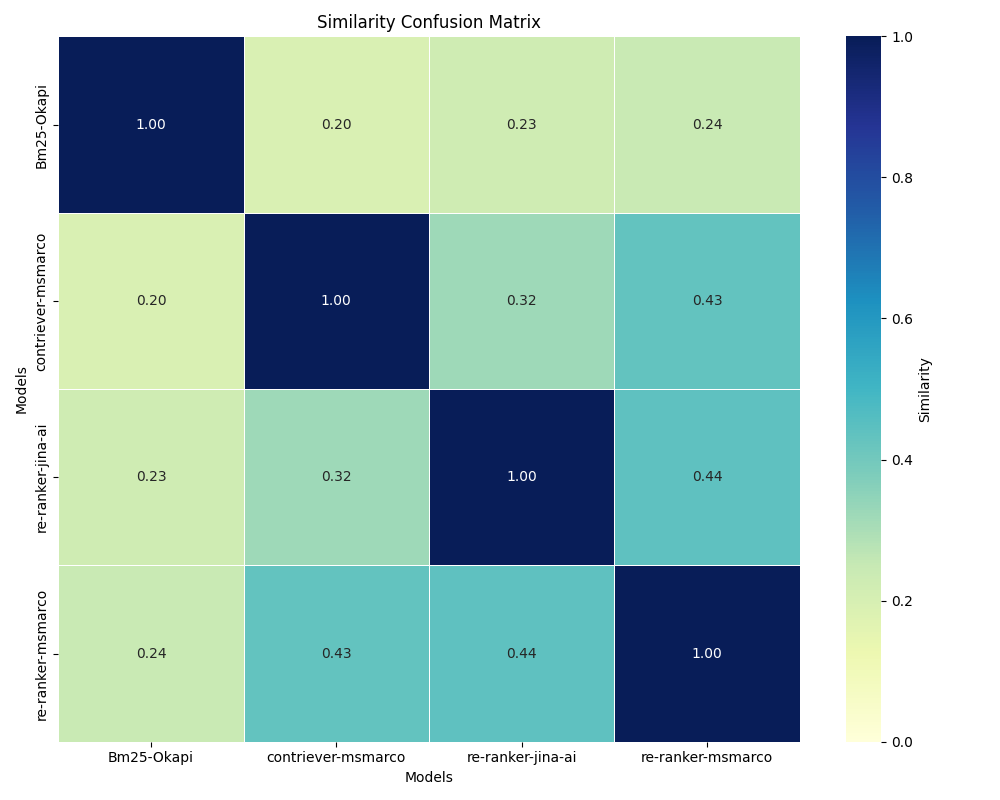
\includegraphics[width=\textwidth]{res/ret_result_sim_1}
    \end{minipage}
    \caption{Document Retrieval Confusion Matrix based on Jaccard Similarity between documents retrieved by each model.}
    \label{fig:document_retrieval_confusion_matrix}
\end{figure}
We can figure out that Bm25-Okapi stands out as the most distinct model, with low similarity scores (0.20-0.24) to the others, suggesting it employs fundamentally different retrieval mechanisms.
In contrast, the neural models show higher inter-model similarities, indicating shared approaches or architectures.
The strong relationship (0.43) between \textit{contriever-msmarco} and \textit{re-ranker-msmarco}, likely due to shared training data or similar optimizations.
The two re-ranker models gain the highest similarity (0.44), highlighting more consistent retrieval patterns.
However, they still exhibit differences in document selection.
In general, we can find out with different methods we have different result over the same query.
To assess the quality of the retrieved documents from each of the above methods, we are passing them through one of our models and evaluating the outputs.

\begin{table}[h!]
    \centering
    \noindent
    \caption{Performance evaluation of various document retrieval methods on the FactBench dataset, using the Gemma2 model.}
    {\scriptsize \fbox{\textit{Retrieval Method}}}\\
    \resizebox{0.7\textwidth}{!}{
        \begin{threeparttable}
        \begin{tabular}{lccc}
            \toprule
            \textbf{Method} & Acc & F1 & Latency\tnote{*} \\
            \midrule
            \textit{Unsupervised}               & & & \\
            Bm25                                & 0.8882          & 0.8940          & \textbf{0.4614s} \\
            contriever-msmarco                  & 0.8932          & 0.8988          & 25.903s \\
            \hline
            \textit{supervised}                 & & & \\
            jina-reranker-v2-base-multilingual  & 0.9004          & 0.9065          & 9.8958s \\
            ms-marco-MiniLM-L-6-v2              & \textbf{0.9014} & \textbf{0.9077} & 0.8172s \\
            \bottomrule
        \end{tabular}
        \begin{tablenotes}
            \item[*] It is measured in seconds on average per query.
        \end{tablenotes}
        \end{threeparttable}}
    \label{tab:evaluation_results}
\end{table}

The empirical results indicate that the model \textit{ms-marco-MiniLM-L-6-v2} achieved the highest F1 score, thus demonstrating superior performance among the evaluated models.
However, it is noteworthy that the performance metrics across all models were closely clustered, suggesting that even traditional methodologies applied within our pipeline yield satisfactory outcomes.

It is crucial to emphasize the significance of data quality in this context, as it substantially influences the efficacy of the results.
To validate the factual accuracy of the knowledge graph, we employed a multi-query information fetching through web search engines for each fact.
This approach provides a reasonable degree of verification for the facts contained within the knowledge graph.

For subsequent evaluations and analyzes, we will designate the model \textit{ms-marco-MiniLM-L-6-v2} as our baseline for retrieval tasks.
This decision is predicated on its superior accuracy and F1 score relative to the other models under consideration with acceptable latency.


\section{Embedding Models}\label{sec:embedding-models}
Text embeddings are dense vector representations that capture the semantic meaning and relationships between words, sentences, or documents in a low-dimensional space.
By mapping text to a continuous vector space, embeddings enable efficient similarity computations and have become a fundamental building block for many NLP applications, such as information retrieval, text classification, clustering, and semantic search.
This section provides an in-depth analysis and comparison of five state-of-the-art text embedding models:

\begin{itemize}
    \item Alibaba-NLP/gte-large-en-v1.5
    \item jinaai/jina-embeddings-v3
    \item dunzhang/stella\_en\_1.5B\_v5
    \item Nextcloud-AI/multilingual-e5-large-instruct
    \item BAAI/bge-small-en-v1.5
\end{itemize}

These models leverage recent advancements in transformer architectures, contrastive learning, and instruction fine-tuning to produce high-quality, general-purpose embeddings that excel across a wide range of downstream tasks.
We examine their model architectures, training methodologies, supported features, and empirical performance on standard benchmarks.
Through this comparative study, we aim to provide insights and guidance for practitioners to select the most suitable embedding model based on their specific use case and computational constraints.

\subsection{Gte-large-en-v1.5}\label{subsec:alibaba-nlp}
The Alibaba-NLP model \textit{gte-large-en-v1.5} is text embedding model designed for general text representation and retrieval tasks.
It is built upon a Transformer++ encoder architecture, combining the strengths of BERT~\cite{devlin2019bertpretrainingdeepbidirectional} with advanced techniques such as \ac{RoPE}~\cite{su2023roformerenhancedtransformerrotary} and Gated Linear Units (GLU).
This combination allows for highly efficient text encoding over long sequences, with a maximum context length of 8192 tokens, significantly surpassing previous models restricted to shorter context lengths (up to 512 tokens)~\cite{zhang2024mgtegeneralizedlongcontexttext}.

One of the major improvements in the gte-v1.5 series is its ability to process long-context text inputs, making it ideal for complex text retrieval and re-ranking tasks~\cite{li2023generaltextembeddingsmultistage}.
This series of models has demonstrated superior performance in multiple benchmarks, including the \ac{MTEB}~\cite{muennighoff-etal-2023-mteb} and the LoCo long-context retrieval benchmark~\cite{saadfalcon2024benchmarkingbuildinglongcontextretrieval}.
In particular, the tuned models of this model ranked second on the MTEB leaderboard and first in the Chinese version of MTEB (C-MTEB).

The model achieves these results by employing a hybrid architecture, including both a text representation model (TRM) and a cross-encoder reranker.
The TRM generates dense text embeddings for retrieval tasks, while the reranker refines results through more precise scoring of candidate texts.
This architecture is optimized for efficiency, allowing faster inference while maintaining high accuracy during both pretraining and fine-tuning stages.

The \textit{gte-large-en-v1.5} also includes instruction-tuned variants, such as \textit{gte-Qwen1.5-7B-instruct}, which is particularly effective for multilingual text embeddings, leveraging a wide range of unsupervised and supervised contrastive learning techniques.
These instruction-tuned models have outperformed various other large embedding models, making them highly suitable for industrial applications that require efficient, accurate text representation across diverse languages.

In summary, the \textit{gte-large-en-v1.5} model stands out in its category due to its ability to handle large context lengths, its efficient encoding techniques, and its strong performance on long-context benchmarks.
This makes it an invaluable tool for a variety of text retrieval, classification, and representation tasks in both academic research and real-world applications.

\subsection{Jina-embeddings-v3}\label{subsec:jinaai}
The \textit{Jina-embeddings-v3} model is a cutting-edge multilingual text embedding solution, developed by Jina AI, aimed at addressing a wide range of \ac{NLP} tasks.
Based on the \textit{Jina-XLM-RoBERTa} architecture, this model supports long-context inputs, handling sequences of up to 8192 tokens thanks to its integration of \ac{RoPE}~\cite{su2023roformerenhancedtransformerrotary,sturua2024jinaembeddingsv3multilingualembeddingstask}.

This ability to process extended sequences makes the model well-suited for tasks such as text retrieval, clustering, classification, and text matching across multiple languages.
One of the key innovations of \textit{Jina-embeddings-v3} is the introduction of task-specific \ac{LoRA}~\cite{hu2022lora} adapters.
These adapters are used to tailor the model's embeddings to specific tasks, such as query-document retrieval, clustering, re-ranking, and classification.
This task-specific optimization is achieved without significantly increasing the model's parameter size.

The model excels in multilingual environments, supporting wide range of languages, and is optimized for performance in long-context retrieval tasks.
Compared to LLMs like \textit{e5-mistral-7b-instruct}, \textit{jina-embeddings-v3} offers a more efficient solution with fewer parameters (570 million \vs 7.1 billion), while still achieving competitive or superior performance on several benchmarks.
For example, it surpasses proprietary models like OpenAI~\footnote{\url{https://openai.com/}} and Cohere~\footnote{\url{https://cohere.com/}} on English tasks and achieves high scores on multilingual benchmarks.

\textit{Jina-embeddings-v3} also features flexible \ac{MRL}~\cite{kusupati2024matryoshkarepresentationlearning}, allowing users to reduce the embedding size from 1024 to as low as 16 dimensions, making it adaptable to different resource constraints without significant loss of performance.

\subsection{Stella\_en\_1.5B\_v5}\label{subsec:dunzhang}
The Dunzhang \textit{Stella\_en\_1.5B\_v5}\footnote{\url{https://huggingface.co/dunzhang/stella_en_1.5B_v5}} is a powerful multilingual text embedding model, built upon the foundations of \textit{Alibaba-NLP/gte-large-en-v1.5}~\ref{subsec:alibaba-nlp} and \textit{gte-Qwen2-1.5B-instruct}.
This model supports two main prompts for diverse tasks: "s2p" (sentence-to-passage) for information retrieval, and "s2s" (sentence-to-sentence) for semantic textual similarity. 
These prompts simplify its application in NLP tasks, such as retrieving relevant passages or finding semantically similar text based on a given query.

One of the standout features of \textit{Stella\_en\_1.5B\_v5} is its implementation of \ac{MRL}~\cite{kusupati2024matryoshkarepresentationlearning}, allowing the model to output embeddings in multiple dimensions ranging from 512 to 8192, depending on user needs. 
Typically, a 1024-dimensional output offers an optimal balance between performance and efficiency. 
In benchmark tests, the model achieves highly competitive results, with only a minor performance difference between 1024-dimensional and 8192-dimensional embeddings.
The model can be employed using both SentenceTransformers and transformers libraries, supporting flexible input formats. 
It is trained on shorter sequences (up to 512 tokens), making it most effective for short-to-medium-length text tasks. 

\subsection{Multilingual-e5-large-instruct}\label{subsec:nextcloud-ai}
The Multilingual E5-Large-Instruct model is an advanced multilingual text embedding model introduced as part of the E5 model family, which aims to improve the quality and utility of multilingual text embeddings~\cite{wang2024multilinguale5textembeddings}.
It is specifically designed to support a wide range of languages and to deliver robust performance across various tasks such as text retrieval, semantic similarity, and multilingual retrieval.

The E5-Large-Instruct model contains 24 layers and features an embedding size of 1024.
It builds on the \textit{XLM-RoBERTa-large}~\cite{DBLP:journals/corr/abs-1911-02116} architecture, which supports 100 languages, albeit with varying performance depending on the resource richness of the language in question.
The model was initialized from XLM-RoBERTa-large and underwent two key stages of training:
\begin{itemize}
    \item \textbf{Contrastive Pre-training:} The model was pre-trained on approximately 1 billion weakly supervised multilingual text pairs using a InfoNCE contrastive loss with only in-batch negatives, while other hyperparameters remain consistent with the English E5 models.
    \item \textbf{Fine-tuning:} Following pre-training, the model was fine-tuned using high-quality labeled datasets from the E5-mistral paper~\cite{wang2024improvingtextembeddingslarge}. This second stage involved a more supervised approach, optimizing performance across specific tasks. During this phase, instruction-tuning was incorporated, where the model learned to generate better embeddings by using natural language task instructions.
\end{itemize}
The E5-Large-Instruct model was evaluated on BEIR and MTEB benchmarks, and its performance is on par with state-of-the-art English-only models.
Evaluation on the MIRACL~\cite{zhang-etal-2023-miracl} multilingual retrieval benchmark across 16 languages and on Bitext mining tasks across over 100 languages demonstrated its capability to handle diverse languages effectively.
Despite the excellent performance on high-resource languages, the model shows a little degradation in performance for low-resource languages, a common limitation of multilingual models, but still outperforms many other models in this category.
The use of contrastive learning and instruction tuning enables the model to generate highly effective embeddings for information retrieval tasks.
\subsection{bge-small-en-v1.5}\label{subsec:baai}
The \textit{\textit{bge-small-en-v1.5}} model is part of the BGE (BAAI General Embeddings) series developed by the Beijing Academy of Artificial Intelligence~\cite{bge_embedding}.
It is a compact English-specific model with just 33.4M parameters, making it highly efficient for deployment in resource-constrained environments.
The model architecture is BERT-like which goes through three-stage of training.
\textit{\textit{bge-small-en-v1.5}} follows a two-stage training pipeline similar to other BGE models:
\begin{itemize}
    \item \textbf{Pre-training:} Weakly-supervised contrastive pre-training on large-scale web data
    \item \textbf{Fine-tuning:} Supervised fine-tuning on a curated set of high-quality English NLP datasets
\end{itemize}

The model fine-tuned using a process of contrastive learning, where sentences are embedded to prioritize semantic similarity.
This technique enhances retrieval tasks by training the model to produce high similarity scores for semantically related sentences while keeping unrelated pairs distant in embedding space.
The fine-tuning emphasizes retrieval for short queries to long passages, optimized with a contrastive loss function and often utilizes mined hard negatives to improve differentiation between similar and unrelated sentence pairs.

Despite its small size, \textit{\textit{bge-small-en-v1.5}} punches above its weight on several English benchmarks and outperforms the base-sized BERT and RoBERTa models on most tasks while being more compact.
The model's strong performance can be attributed to the efficient architecture design and the use of high-quality fine-tuning data.
It presents an attractive option for applications requiring low-latency inference or deployment on edge devices.

\subsection{Comparative Analysis}\label{subsec:comparative-analysis}
We examine their model size and efficiency, language coverage, supported features, and overall performance to provide insights for selecting the most suitable model based on specific requirements.

\subsubsection{Model Size and Efficiency}
Table~\ref{tab:comparison-embeddings} compares the model size, memory usage, embedding dimensions, and maximum token length of the five models. 
The \textit{stella\_en\_1.5B\_v5} model has the largest size with 1,543 million parameters, while \textit{bge-small-en-v1.5} is the smallest with only 33 million parameters.
Larger models generally require more memory and computational resources, which may be a consideration for resource-constrained environments.
In terms of memory usage, \textit{stella\_en\_1.5B\_v5} requires 5.75 GB in fp32 precision, while \textit{bge-small-en-v1.5} only needs 0.12 GB.
This substantial difference in memory footprint can be a decisive factor when deploying models on edge devices or serving them in real-time applications with limited resources.
The embedding dimensions also vary among the models, ranging from 384 for \textit{bge-small-en-v1.5} to 8192 for \textit{stella\_en\_1.5B\_v5}.
Higher-dimensional embeddings can capture more fine-grained semantic information but may increase storage requirements and similarity computation costs.
Practitioners should consider the trade-off between embedding quality and efficiency based on their specific use case.

\begin{table}[ht!]
    \centering
    \noindent
    \caption{Comparison of characteristics of embedding models}
    \resizebox{\textwidth}{!}{
        \begin{tabular}{lcccc}
            \toprule
            \textbf{Model} & \shortstack{\textbf{Model Size} \\ (Million Parameters)}           & \shortstack{\textbf{Memory Usage} \\ (GB, fp32)}             & \shortstack{\textbf{Embedding}  \\ \textbf{Dimensions}}              & \shortstack{\textbf{Max}  \\ \textbf{Tokens}} \\
            \midrule
            stella\_en\_1.5B\_v5                & 1543  & 5.75  & 8192  & 131072    \\
            jina-embeddings-v3                  & 572   & 2.13  & 1024  & 8194      \\
            gte-large-en-v1.5                   & 434   & 1.62  & 1024  & 8192      \\
            multilingual-e5-large-instruct      & 560   & 2.09  & 1024  & 514       \\
            bge-small-en-v1.5                   & 33    & 0.12  & 384   & 51262     \\
            \bottomrule
        \end{tabular}}
    \label{tab:comparison-embeddings}
\end{table}

\subsubsection{Language Coverage}
Language coverage is a crucial aspect when selecting an embedding model for multilingual applications. The \textit{Multilingual-e5-large-instruct} model stands out in this regard, as it supports a wide range of languages.
This model leverages instruction fine-tuning on multilingual data, enabling it to generate high-quality embeddings for various languages.
The \textit{Jina-embeddings-v3} model also offers multilingual support, although the exact language coverage is not specified in the provided context. On the other hand, the \textit{Bge-small-en-v1.5}, \textit{Stella\_en\_1.5B\_v5}, and \textit{Gte-large-en-v1.5} models primarily focus on English embeddings, making them more suitable for monolingual English applications.
\subsubsection{Conclusion}
The choice of text embedding model depends on various factors, including the specific application, language coverage requirements, available computational resources, and desired features. For monolingual English applications, the \textit{Gte-large-en-v1.5} and \textit{Stella\_en\_1.5B\_v5} models offer high-quality embeddings with support for longer input sequences.
The \textit{Stella\_en\_1.5B\_v5} model, in particular, provides prompt-based adaptability for information retrieval and semantic similarity tasks.
For multilingual applications, the \textit{Multilingual-e5-large-instruct} and \textit{Jina-embeddings-v3} models are strong contenders.
The \textit{Multilingual-e5-large-instruct} model supports a wide range of languages, while \textit{Jina-embeddings-v3} offers task-specific LoRA adapters for enhanced performance across various NLP tasks.
When computational resources are limited, the \textit{Bge-small-en-v1.5} model presents a lightweight option with competitive performance.
Its small size and low memory footprint make it suitable for deployment on edge devices or real-time applications.
Ultimately, we should carefully evaluate our specific requirements and constraints before selecting an embedding model.
The comparative analysis provided in this section aims to assist in this decision-making process by highlighting the key differences and strengths of each model.
Now we will test these models through the pipeline and evaluate their performance.

\begin{table}[h!]
    \centering
    \noindent
    \caption{Performance evaluation of various embedding models on the FactBench dataset, using the Gemma2 model.}
    {\scriptsize ms-marco-MiniLM-L-6-v2,\fbox{\textit{Embedding Model}}}\\
    \resizebox{0.7\textwidth}{!}{
        \begin{threeparttable}
        \begin{tabular}{lccc}
            \toprule
            \textbf{Model} & Acc & F1 & Latency \\
            \midrule
            stella\_en\_1.5B\_v5                  & 0.8961          & 0.9028          & 17.692s \\
            multilingual-e5-large-instruct        & 0.8954          & 0.9018          & 5.0038s \\
            bge-small-en-v1.5                     & \textbf{0.9014} & 0.9077          & \textbf{1.6958s} \\\hline
            \rowcolor{gry}
            jina-embeddings-v3\tnote{*}           & 0.8852          & 0.9097          & 4.8745s \\
            \rowcolor{gry}
            gte-large-en-v1.5\tnote{*}            & 0.8971          & \textbf{0.9174} & 5.8571s \\
            \bottomrule
        \end{tabular}
        \begin{tablenotes}
            \item[*] The models were not able to complete the evaluation due to memory constraints, Jina evaluated on the 2238/2800 and Gte-large evaluated on the 2322/2800.
        \end{tablenotes}
    \end{threeparttable}}
    \label{tab:evaluation_results_embedding}
\end{table}

Based on the Table~\ref{tab:evaluation_results_embedding}, we use the \textit{bge-small-en-v1.5} model for the subsequent evaluations and analyses due to its superior performance across F1 and accuracy metrics.
The low latency of 1.6958 seconds per query also makes it an attractive choice for real-time applications.
The F1 score of \textit{gte-large-en-v1.5} is slightly higher, but the model is not able to complete the evaluation due to memory limitations in the same pipeline.

\section{Chunking Strategies}\label{sec:chunking-strategies}
A critical component of \ac{RAG} systems is the chunking strategy employed to divide documents into smaller, manageable pieces for efficient retrieval and processing.
This section examines three distinct chunking methods for \ac{RAG} systems, each with its unique characteristics and potential advantages.

\subsection{Parsing Documents into Text Chunks}\label{subsec:parsing-documents-into-text-chunks}
The first method we will explore involves parsing documents into text chunks, also referred to as nodes, of fixed sizes.
This approach is straightforward and widely used in many RAG implementations.
We will investigate three different chunk sizes: 256, 512, and 1024 tokens.
\subsubsection{Methodology}
In this method, documents are sequentially divided into chunks of the specified size.
If the final chunk is smaller than the designated size, it is typically padded or left as is, depending on the implementation.
\subsubsection{Chunk Sizes}
\begin{itemize}
    \item \textbf{256-token chunks:} This size offers fine granularity, potentially allowing for more precise retrieval of relevant information. However, it may result in a loss of context for more complex topics that require broader context.
    \item \textbf{512-token chunks:} This medium-sized chunk strikes a balance between granularity and context preservation. It is often considered a good default choice for many applications.
    \item \textbf{1024-token chunks:} Larger chunks preserve more context but may retrieve more irrelevant information and increase computational overhead during retrieval and processing.
\end{itemize}

\subsection{Smaller Child Chunks Referring to Bigger Parent Chunks (Small2Big)}\label{subsec:smaller-child-chunks-referring-to-bigger-parent-chunks}
The second method, which we will refer to as \textit{Small2Big}, involves creating a hierarchical structure of chunks, where smaller child chunks refer to larger parent chunks.
This approach aims to combine the benefits of fine-grained retrieval with the context preservation of larger chunks.
\subsubsection{Methodology}
In this method, we parsed documents into three levels of chunks with appending the original text chunk of size 1024:
\begin{itemize}
    \item Smallest children: 128-token chunks
    \item Intermediate parents: 256-token chunks
    \item Largest parents: 512-token chunks
\end{itemize}
Each smaller chunk maintains a reference to its parent chunks, allowing the system to retrieve additional context when needed.

\begin{lstlisting}[language=Python, caption=Small2Big Chunking Method, label=lst:small2big_chunking]
# ...previous code
sub_chunk_sizes = [128, 256, 512]
sub_node_parsers = [SimpleNodeParser.from_defaults(chunk_size=c) for c in sub_chunk_sizes]

all_nodes = []
for base_node in base_nodes:
    for n in sub_node_parsers:
        sub_nodes = n.get_nodes_from_documents([base_node])
        sub_inodes = [
            IndexNode.from_text_node(sn, base_node.node_id) for sn in sub_nodes
        ]
        all_nodes.extend(sub_inodes)

    original_node = IndexNode.from_text_node(base_node, base_node.node_id) # also add original node to node
    all_nodes.append(original_node)
all_nodes_dict = {n.node_id: n for n in all_nodes}
# ... continue processing
\end{lstlisting}

\subsection{Sentence Window Retrieval}\label{subsec:sentence-window-retrieval}
The third method, Sentence Window Retrieval, focuses on maintaining semantic coherence by chunking based on sentences and incorporating surrounding context through windows.
\subsubsection{Methodology}
In this approach, documents are first split into individual sentences.
For each sentence, a \textit{window} of surrounding sentences is included to provide context.
we use the \textit{SentenceWindowNodeParser} to parse documents into single sentences per node.
\begin{figure}[ht!]
    \centering
    \begin{minipage}[b]{\textwidth}
        \centering
        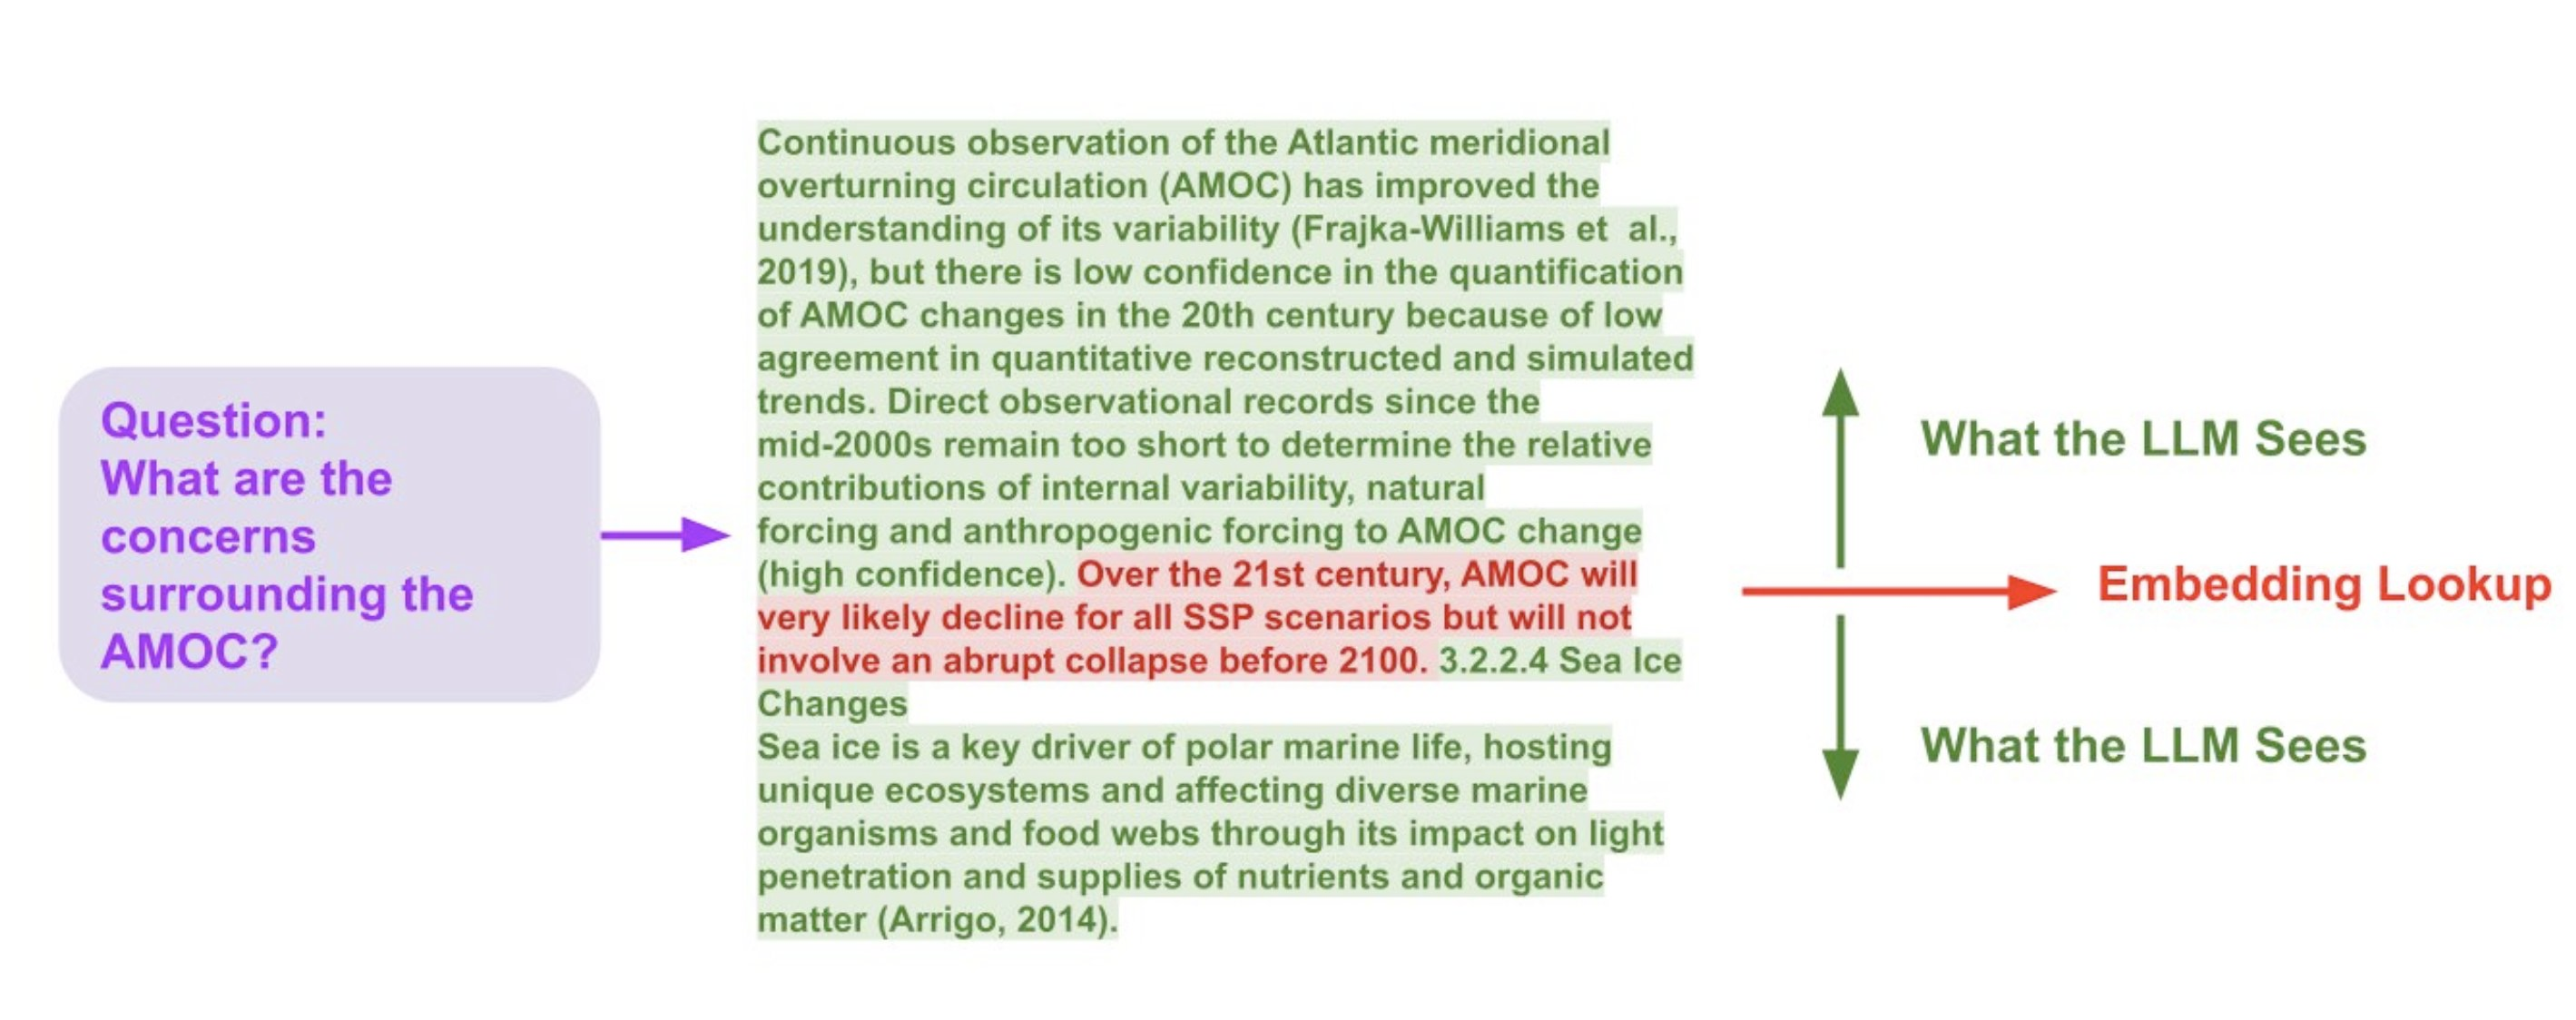
\includegraphics[width=\textwidth]{res/window-ret}
        \caption{Node sentence window replacement technique as described by Liu~\cite{liu2023tweet}.}
        \label{fig:window-ret}
    \end{minipage}
\end{figure}
Each node also contains a \textit{"window"} with the sentences on either side of the node sentence.
Then, after retrieval, before passing the retrieved sentences to the LLM, the single sentences are replaced with a window containing the surrounding sentences using the MetadataReplacementNodePostProcessor.
This is most useful for large documents/indexes, as it helps to retrieve more fine-grained details.
We will examine two window sizes: 3 and 6.
%There is example of the \textit{SentenceWindowNodeParser} and \textit{MetadataReplacementNodePostProcessor} in the Appendix~\ref{ch:chunking}.
\subsection{Advantages and Limitations}\label{subsec:advantages-and-limitations}
Table~\ref{tab:window-segmentation-analysis} provides an analysis of the advantages and limitations of each text segmentation method based on their methodological approach.
Each of the three chunking methods presented in this section offers distinct advantages and limitations for RAG systems.
The choice of method depends on factors such as the nature of the documents, the specific requirements of the application, and the computational resources available.
The fixed-size chunking method provides simplicity and consistency but may sacrifice semantic coherence.
The Small2Big hierarchical approach offers flexibility in retrieval granularity but introduces complexity in implementation and storage.
Sentence Window Retrieval preserves semantic units and adapts to text structure but may result in variable chunk sizes.

Examples of the three chunking methods are available in the Appendix~\ref{ch:chunking} for further reference.

\begin{table}[h!]
    \footnotesize
    \caption{Advantages and Limitations of different chunking strategies for RAG systems.}
    \begin{xltabular}{\linewidth}{lXX}
        \toprule
        \textbf{Method} & \textbf{Advantages} & \textbf{Limitations} \\
        \midrule
        \multirow{5}{*}{Fixed Chunking} &
        $\ast$ Simple to implement and understand \newline
        $\ast$ Consistent chunk sizes facilitate uniform processing
        &
        $\ast$ Fixed chunk sizes may not align with natural breaks in the text \newline
        $\ast$ Larger chunks can introduce irrelevant information and increase computational costs
        \\ \hline
        \multirow{5}{*}{Small2Big} &
        $\ast$ Allows for fine-grained retrieval with the option to expand context \newline
        $\ast$ Adapts to different levels of specificity required by queries
        &
        $\ast$ More complex to implement and manage \newline
        $\ast$ Increased storage requirements due to redundancy in the hierarchy
        \\\hline
        \multirow{5}{*}{Sentence Window} &
        $\ast$ Preserves semantic units (sentences) and their immediate context \newline
        $\ast$ Adapts to the natural structure of the text
        &
        $\ast$ Variable chunk sizes may complicate processing and indexing \newline
        $\ast$ Optimal window size may vary depending on the document type and content \\
        \bottomrule
    \end{xltabular}
    \label{tab:window-segmentation-analysis}
\end{table}

\subsection{Evaluation}\label{subsec:evaluation}
The Table~\ref{tab:table_chunking} illustrates that as the chunk size increases, there is a minor downtick in the average latency.
Consider that the pipeline's average response time increases as the chunk size increases, which is expected as the model has to process more tokens.
Interestingly, the faithfulness (\ie measuring how closely response is aligned with the source material) seems to reach its zenith at chunk\_size of 1024, whereas average relevancy shows a consistent improvement with larger chunk sizes, also peaking at 1024.
This suggests that a chunk size of 1024 might strike an optimal balance between response time and the quality of the responses, measured in terms of faithfulness and relevancy.
In the sliding window method, the window size of 3 outperforms the window size of 6 in terms of both accuracy and F1 score, while maintaining nearly the same average response time.
We can figure out that the baseline accuracy and F1 scores across chunking strategies indicate that the model’s performance is largely unaffected by these variations, suggesting that factors other than chunk size, may have a more significant impact on the retrieval process.
\begin{table}[h!]
    \centering
    \noindent
    \caption{Performance evaluation of various chunking strategy on the FactBench dataset, using the Gemma2 model.}
    {\scriptsize ms-marco-MiniLM-L-6-v2, BAAI/bge-small-en-v1.5,\fbox{\textit{Chunking Strategy}}}\\
    \resizebox{0.75\textwidth}{!}{
        \begin{tabular}{llccc}
            \toprule
            \textbf{Method} & \textbf{Parameters} & Acc & F1 & Latency \\
            \midrule
            \multirow{3}{*}{Original}           & Chuck Size: 256       & 0.8914          & 0.8914          & 0.04473s \\
                                                & Chuck Size: 512       & 0.8932          & 0.8993          & 0.02670s \\
                                                & Chuck Size: 1024      & 0.8946          & 0.8993          & \textbf{0.02378s} \\ \hline
            small2big                           & Chuck Size: 1024      & 0.8889          & 0.8953          & 0.19188s \\ \hline

            \multirow{2}{*}{Sliding Window}     & Window Size: 3        & \textbf{0.9014} & \textbf{0.9080} & 0.03076s \\
                                                & Window Size: 6        & \textbf{0.9014} & 0.9077          & 0.03534s \\
            \bottomrule
        \end{tabular}}
    \label{tab:table_chunking}
\end{table}

We chose the Sliding Window with window size 3 method as it provides the surrounding context of the text and has the highest F1 score and accuracy.

\section{Similarity Cut-off}\label{sec:similar-cut-off}
In this section we will discuss how similarity cut-off can be used to filter out irrelevant nodes and improve the efficiency of the retrieval process.
We use Node postprocessors to apply a similarity cut-off to the retrieved nodes, discarding those with a similarity score below a certain threshold.
Node postprocessors are a set of modules that take a set of nodes, and apply some kind of transformation or filtering before returning them.
For our experiments, we set the similarity cut-off threshold to 0.3, meaning that nodes with a similarity score below 0.3 are discarded, we use the naive score and the re-ranker score to compare the results.
The Algorithm~\ref{alg:algorithm} shows the similarity cut-off postprocessor implementation.
\begin{algorithm}
    \begin{algorithmic}[1]
        \Procedure{PostprocessNodes}{nodes, knowledge\_graph, similarity\_cutoff}
            \State $new\_nodes \gets []$
            \State $node\_texts \gets [node.text \text{ for } node \text{ in } nodes]$
            \State $re\_rank\_nodes \gets \textsc{ReRank}(knowledge\_graph, node\_texts)$

            \For{each $node$ in $nodes$}
                \State $node.score \gets \text{get\_node\_score}(node.text, re\_rank\_nodes)$

                \If{$node.score > similarity\_cutoff$}
                    \State $new\_nodes.\textsc{Append}(node)$
                \EndIf
            \EndFor

            \State \Return $new\_nodes$
        \EndProcedure
    \end{algorithmic}
    \caption{Similarity Cutoff Postprocessor (re-rank score)}\label{alg:algorithm}
\end{algorithm}

\begin{table}[h!]
    \centering
    \noindent
    \caption{Performance evaluation of similarity cut-off method on the FactBench dataset, using the Gemma2 model.}
    {\scriptsize ms-marco-MiniLM-L-6-v2, BAAI/bge-small-en-v1.5, Sliding Window (ws 3), \fbox{\textit{Similarity Cut-off}}}\\
    \resizebox{0.7\textwidth}{!}{
        \begin{threeparttable}
            \begin{tabular}{lccc}
                \toprule
                \textbf{Method} & Acc & F1 & Latency Diff.\tnote{*} \\
                \midrule
                \rowcolor{LightGreen}
                w/o similarity cut-off (baseline)                       & 0.8971          & 0.9036                  &  -- \\\hline
                similarity cut-off (original score)                     & \textbf{0.9018} & \textbf{0.9080}         & -0.22237s \\
                similarity cut-off (re-ranked score)                    & 0.9014          & \textbf{0.9080}         & -0.350783 \\
                \bottomrule
            \end{tabular}
            \begin{tablenotes}
                \item[*] The latency is compared to the baseline without the similarity cut-off on average per query.
            \end{tablenotes}
        \end{threeparttable}}
    \label{tab:table_similarity_cut}
\end{table}

Based on the results in Table~\ref{tab:table_similarity_cut}, we decided to apply a similarity cut-off with the original score to provide the model with higher-quality data for further evaluations.
This approach yields the highest accuracy and F1 score, though it is slightly slower than the re-ranker mode because it removes fewer irrelevant nodes.
A drawback of re-ranking is that it may eliminate all relevant nodes based on low similarity score, requiring a re-run without the similarity cut-off, which increases processing time (not shown in the Table~\ref{tab:table_similarity_cut}).
In separate evaluations (not reported in Table~\ref{tab:table_similarity_cut}), we also tested a normalized similarity cut-off using re-ranked scores scaled between the original minimum and maximum values.
However, this normalized approach did not perform as well as the original scores.

\section{Top K}\label{sec:top-k}
Top\_k mentions how many top embeddings to take into context.
Considering a large top\_k might go beyond the max\_tokens of the model, we will evaluate the performance of the pipeline with the top\_k set to 3 and 6, and compare the results to determine the optimal value for this parameter.
\begin{table}[h!]
    \centering
    \noindent
    \caption{Performance evaluation of different Top\_k retrieval strategies on the FactBench dataset using the Gemma2 model. }
    {\scriptsize ms-marco-MiniLM-L-6-v2, BAAI/bge-small-en-v1.5, Sliding Window (ws 3), Similarity Cut-off (Original),\fbox{\textit{Top\_k}}}
    \resizebox{0.45\textwidth}{!}{
        \begin{threeparttable}
        \begin{tabular}{lccc}
            \toprule
            \textbf{Method} & Acc & F1 & Latency\tnote{*} \\
            \midrule
            Top\_k 3                     & 0.9018               & 0.9080                    & \textbf{5.21177s} \\
            Top\_k 6                     & \textbf{0.9032}      & \textbf{0.9101}           & 7.02713s \\
            \bottomrule
        \end{tabular}
        \begin{tablenotes}
            \item[*] The latency represents the average time per query for a complete run.
        \end{tablenotes}
        \end{threeparttable}}
    \label{tab:table_top_k}
\end{table}
\newline
As we decided to set the similarity cut-off with 0.3 threshold, it's good to use the top\_k 6 to have more high-quality embeddings in the context, and based on results on Table~\ref{tab:table_top_k} it outperforms the top\_k 3, so we will use top\_k 6 for subsequent evaluations.
The difference in latency is significant, presenting a trade-off between more data and response time.
Since the quality of data for additional facts is uncertain, we aim to include more data in the context.

\section{Evaluation}\label{sec:evaluation-and-discussion}
In this ablation study, we evaluate the performance of the merging method, which leverages a novel ensemble approach by combining multiple models (\textit{Gemma2}, \textit{Qwen2.5}, \textit{Llama3.1}, and \textit{Mistral}) to show the robustness and accuracy of the pipeline.
As presented in Tables~\ref{tab:evaluation_results-full-category} and~\ref{tab:evaluation_results-full-wo-category}, along with Figure~\ref{fig:radar-charts}, the proposed ensemble method consistently outperforms individual models across both positive and negative labels, achieving a more balanced and comprehensive performance.

Note that the ensemble method is based on the tie-breaking strategy discussed in Section~\ref{subsec:conflict-resolution-strategies}, with \textit{At\_Most} as the merging method.
Based on the provided configurations the model selected for \textit{At\_Most} methodology is the \textit{Gemma2:21B}.

\begin{figure}[ht!]
    \centering
    \begin{minipage}[b]{0.4\textwidth}
        \centering
        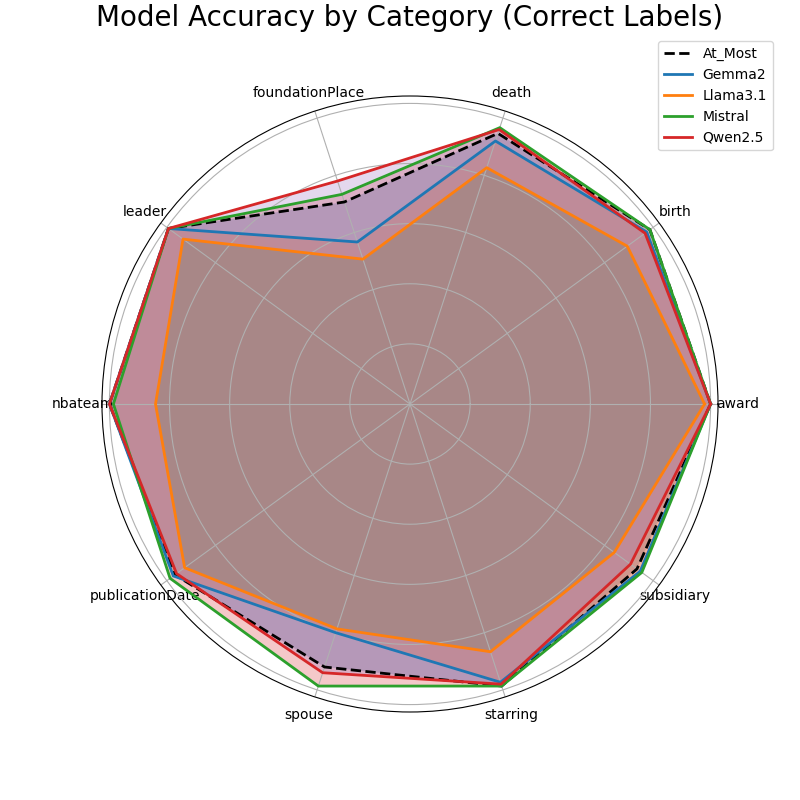
\includegraphics[width=\textwidth]{res/combined_correct_radar_chart}
    \end{minipage}
    \hspace{0.05\textwidth} % Space between the images
    \begin{minipage}[b]{0.4\textwidth}
        \centering
        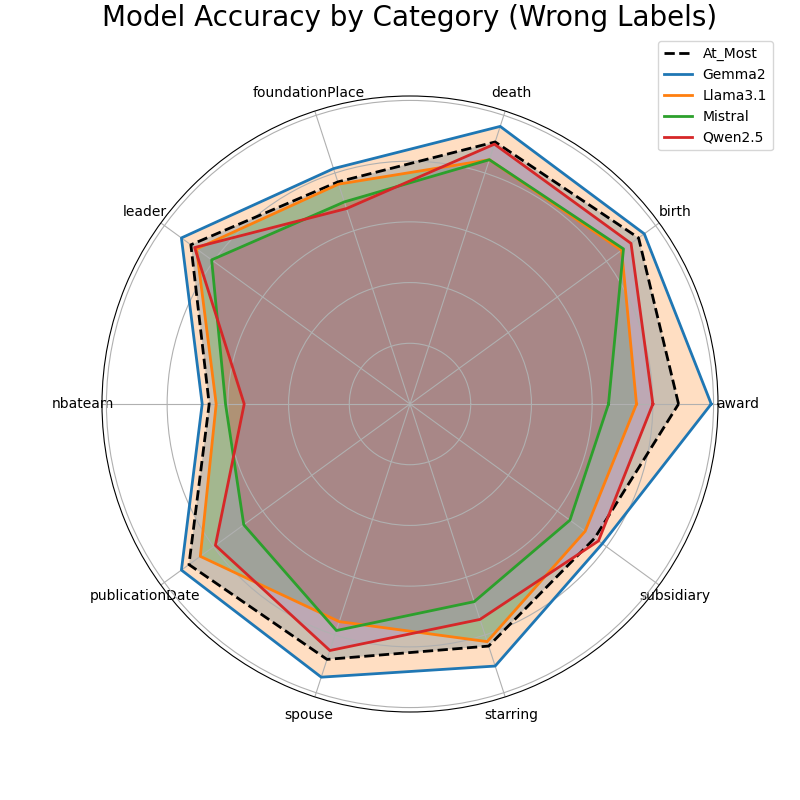
\includegraphics[width=\textwidth]{res/combined_wrong_radar_chart}
    \end{minipage}
    \caption{Category-wise performance of different models in identifying Positive Labels (left) and Negative Labels (right) on the FactBench dataset.}
    \label{fig:radar-charts}
\end{figure}

\begin{table}[h!]
    \noindent
    \caption{Category-wise performance evaluation results of various models on the FactBench dataset.}
    {\scriptsize ms-marco-MiniLM-L-6-v2, BAAI/bge-small-en-v1.5, Sliding Window (ws 3), Similarity Cut-off (Original), Top\_k 6}
    \resizebox{\textwidth}{!}{
        \begin{tabular}{lcccccccccc||c}
            \toprule
            \textbf{Model}                     & \begin{sideways}award\end{sideways}                     & \begin{sideways}birth\end{sideways}                     & \begin{sideways}death\end{sideways}                     & \begin{sideways}foundationPlace\end{sideways}                     & \begin{sideways}leader\end{sideways}                    & \begin{sideways}nbateam\end{sideways}                     & \begin{sideways}publicationDate\end{sideways}                     & \begin{sideways}spouse\end{sideways}                    & \begin{sideways}starring\end{sideways} & \begin{sideways}subsidiary\end{sideways} & \begin{sideways}Total\end{sideways} \\
            \midrule
            \textit{Positive Labels}           &                                                         &                                                         &                                                         &                                                                   &                                                         &                                                           &                                                                   &                                                         &                                        &                                          &       \\
            Gemma2                             & \textbf{1.0000}                                         & 0.9733                                                  & 0.9200                                                  & 0.5667                                                            & \textbf{0.9933}                                         & \textbf{1.0000}                                           & 0.9733                                                            & 0.8000                                                  & 0.9733                                 & 0.9467                                   & 0.9147 \\
            Qwen2.5                            & \textbf{1.0000}                                         & 0.9667                                                  & \textbf{0.9600}                                         & \textbf{0.7800}                                                            & \textbf{0.9933}                                         & \textbf{1.0000}                                           & 0.9600                                                            & 0.9400                                                  & 0.9800                                 & 0.9067                                   & \textbf{0.9487} \\
            Llama3.1                           & 0.9800                                                  & 0.8933                                                  & 0.8267                                                  & 0.5067                                                            & \textbf{0.9333}                                         & 0.8467                                                    & 0.9267                                                            & 0.7867                                                  & 0.8667                                 & 0.8400                                   & 0.8407 \\
            Mistral                            & \textbf{1.0000}                                         & \textbf{0.9867}                                                  & 0.9667                                                  & 0.7333                                                            & \textbf{0.9933}                                         & 0.9867                                                    & \textbf{0.9867}                                                   & \textbf{0.9867}                                                  & \textbf{0.9867}                        & \textbf{0.9533}                          & 0.9580 \\
            Proposed (At\_Most)                & \textbf{1.0000}                                         & \textbf{0.9867}                                                  & 0.9467                                                  & 0.7067                                                            & \textbf{0.9933}                                         & \textbf{1.0000}                                           & 0.9667                                                            & 0.9200                                                  & \textbf{0.9867}                        & 0.9333                                   & 0.9440 \\
            \hline
            \textit{Negative Labels}           &                                                         &                                                         &                                                         &                                                                   &                                                          &                                                           &                                                                  &                                                         &                                        &                                          &       \\
            Gemma2                             & \textbf{0.9923}                                         & \textbf{0.9538}                                         & \textbf{0.9615}                                         & \textbf{0.8154}                                                   & \textbf{0.9308}                                         & \textbf{0.6846}                                           & \textbf{0.9308}                                                   & \textbf{0.9462}                                         & \textbf{0.9077}                        & \textbf{0.7769}                          & \textbf{0.8900} \\
            Qwen2.5                            & 0.8000                                                  & 0.9000                                                  & 0.9000                                                  & 0.6769                                                            & 0.8769                                                  & 0.5462                                                    & 0.7923                                                            & 0.8538                                                  & 0.7462                                 & 0.7615                                   & 0.7854 \\
            LLama3.1                           & 0.7462                                                  & 0.8615                                                  & 0.8462                                                  & 0.7615                                                            & 0.8692                                                  & 0.6385                                                    & 0.8538                                                            & 0.7538                                                  & 0.8231                                 & 0.7077                                   & 0.7862 \\
            Mistral                            & 0.6538                                                  & 0.8692                                                  & 0.8462                                                  & 0.7000                                                            & 0.8077                                                  & 0.6077                                                    & 0.6769                                                            & 0.7846                                                  & 0.6846                                 & 0.6462                                   & 0.7277 \\
            Proposed (At\_Most)                & 0.8846                                                  & 0.9308                                                  & 0.9077                                                  & 0.7692                                                            & 0.8923                                                  & 0.6615                                                    & 0.9000                                                            & 0.8846                                                  & 0.8385                                 & 0.7462                                   & 0.8415 \\
            \bottomrule
        \end{tabular}}
    \label{tab:evaluation_results-full-category}
\end{table}

\begin{table}
    \noindent
    \caption{Performance evaluation of various models on the FactBench dataset.}
    {\scriptsize ms-marco-MiniLM-L-6-v2, BAAI/bge-small-en-v1.5, Sliding Window (ws 3), Similarity Cut-off (Original), Top\_k 6}
    \resizebox{\textwidth}{!}{
        \begin{tabular}{lccc||cc}
            \toprule
            \textbf{Model}                     & \textbf{Consistency}             & \textbf{Avg. Request Duration} & \textbf{Avg. tokens per request}          & \textbf{ACC} & \textbf{F1} \\
            \midrule
            Gemma2                             & 0.8720                         & 5.6826s                            & 1605.29                                       & \textbf{0.9032}    & \textbf{0.9101}   \\
            Qwen2.5                            & 0.8685                         & 6.3094s                            & 1652.66                                       & 0.8729    & 0.8888   \\
            LLama3.1                           & 0.8291                         & 6.5270s                            & 1679.04                                       & 0.8154    & 0.8299   \\
            Mistral                            & 0.8650                         & 4.6692s                            & 1594.76                                       & 0.8511    & 0.8733   \\ \hline
            Proposed (At\_Most)                & \textbf{0.9176}                & 16.815s                            & 1604.196                                      & 0.8964    & 0.9071   \\
            \bottomrule
        \end{tabular}}
    \label{tab:evaluation_results-full-wo-category}
\end{table}

%
%\begin{figure}[ht!]
%    \centering
%    \begin{minipage}[b]{0.4\textwidth}
%        \centering
%        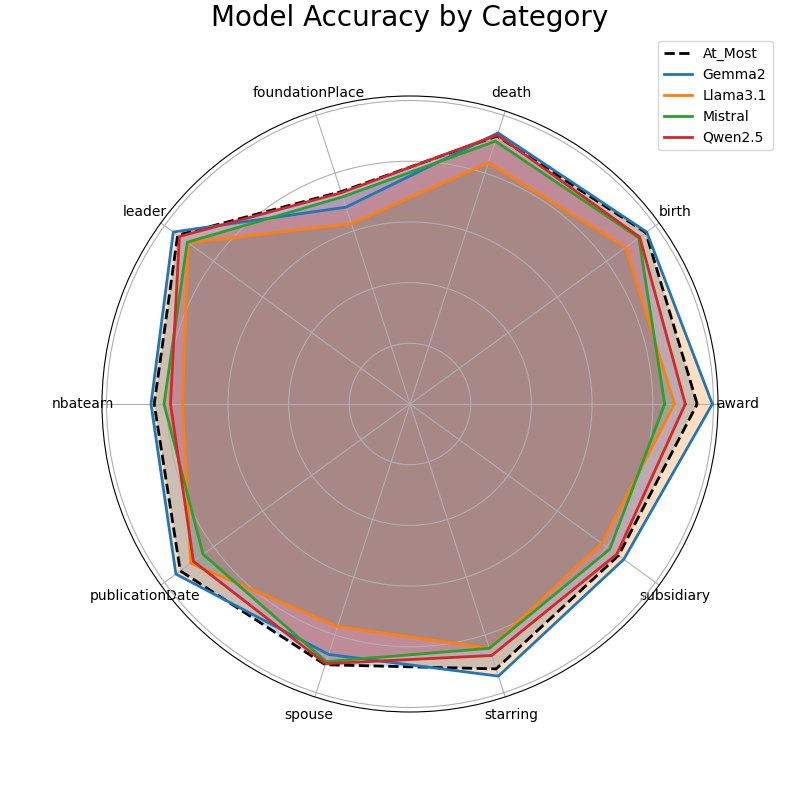
\includegraphics[width=\textwidth]{res/combined_radar_chart}
%    \end{minipage}
%    \caption{Category-wise performance of different models on the FactBench dataset.}
%    \label{fig:all-radar-chart}
%\end{figure}

\section{Failure Analysis}\label{sec:faiure-analysis}
To gain a deeper understanding of the limitations and challenges faced by our fact-checking system, we conducted a comprehensive failure analysis using the \textit{FactBench} dataset.
By examining the instances where our system, based on the majority vote, failed to correctly verify the facts, we aimed to identify the main error types and provide insights into the reasons behind these failures.
\subsubsection{Error Type Categorization}
After analyzing the failure cases, we categorized the errors into four main types:
\begin{itemize}
    \item \textbf{Insufficient or Irrelevant Context:} In some cases, the provided context information does not directly support or refute the given triple. The LLMs struggle to make accurate judgments when the necessary facts are missing or the available information is tangentially related to the claim.
    \item \textbf{Misinterpretation of Relationships:} The LLMs sometimes misinterpret the relationships between entities mentioned in the context. They may confuse family relations, professional associations, or the nature of events.
    \item \textbf{Over reliance on Keyword Matching:} In some instances, the LLMs rely too heavily on surface-level keyword matching rather than understanding the underlying semantics. The presence of certain words or phrases can lead to incorrect assumptions.
    \item \textbf{Lack of Common Sense Reasoning:} The LLMs can struggle with applying common sense knowledge or reasoning about the plausibility of claims. They may fail to consider the unlikelihood of certain scenarios or relationships.
%    \item \textbf{Difficulty with Negation and Contradiction:} The LLMs sometimes struggle with handling negation or identifying contradictions between the triple and the context information. They may overlook explicit denials or fail to recognize inconsistencies.
\end{itemize}

%To quantify the distribution of error types, we classified each error instance into one or more of four categories, allowing for overlaps when errors fit multiple categories.
\begin{table}[h!]
    \footnotesize
    \caption{Example of failure cases and error analysis observed in the FactBench dataset using generated results and explanations.}
    \begin{xltabular}{\linewidth}{p{3cm}p{3cm}X}
        \toprule
        \textbf{Error Type} & \textbf{Triple} & \textbf{Description} \\
        \midrule
        Insufficient or Irrelevant Context & Ai Sugiyama birth place Yokohama & Since there's no information in any of the documents about Ai Sugiyama being born in Yokohama, and one document explicitly states her birthplace as Tokyo. So LLms infer that Ai Sugiyama was born in Tokyo, Japan and not Yokohama, Japan. \\\hline
        Mis Interpretation of Relationships & Mitt Romney office Dallas & LLMs mistakenly infer that Romney has an office in Dallas based on his attendance at a fundraiser there. Attending an event doesn't imply having a permanent office. \\\hline
        Over reliance on Keyword Matching & Robbie Williams office Los Angeles & LLMs wrongly assume Robbie Williams has an office in Los Angeles due to text discussing his purchase or sell of a property there, not an office. \\\hline
        Lack of Common Sense Reasoning & Saul Bellow starring Nobel Prize in Literature & LLMs fail to recognize "starring" is inappropriate for receiving a Nobel Prize. Common sense suggests terms like "awarded" or "received." \\
%        Difficulty with Negation and Contradiction & John William Strutt team Nobel Prize in Physics & LLMs confirm the presence of a team, despite no evidence suggesting Strutt was part of one. The context mentions Strutt’s Nobel Prize but lacks information about team involvement. \\
        \bottomrule
    \end{xltabular}
    \label{tab:factbench-failure-analysis}
\end{table}

Based on Figure~\ref{fig:wrong_prediction_distribution}, The "foundationPlace" relation shows the highest number of total instances and errors in both charts.
This suggests that the model struggles most with verifying facts about the locations where organizations or institutions were founded.
The large discrepancy between correct and incorrect predictions for this relation indicates a significant challenge in accurately processing location-based information.

Relations such as "birth", "death", and "spouse" show varying levels of difficulty.
While "birth" and "death" have relatively few instances, "spouse" has a moderate number of cases with a notable error rate.
This suggests that verifying personal information, especially relationships, poses challenges for the model, and mostly related to having multiple marriages or relationships during a lifetime.

The "nbateam" and "subsidiary" relations, which involve organizational affiliations, show moderate error rates.
This indicates that the model has some difficulty in correctly identifying professional associations and corporate structures.

\begin{figure}[ht!]
    \centering
    \begin{minipage}[b]{0.4\textwidth}
        \centering
        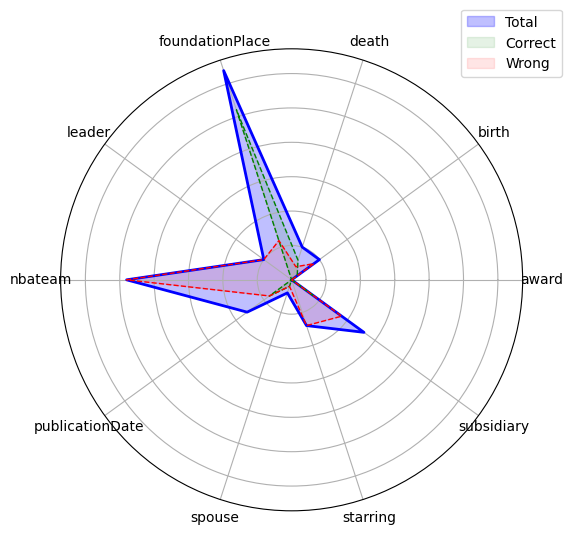
\includegraphics[width=\textwidth]{res/radar-error-0}
    \end{minipage}
    \hspace{0.05\textwidth} % Space between the images
    \begin{minipage}[b]{0.4\textwidth}
        \centering
        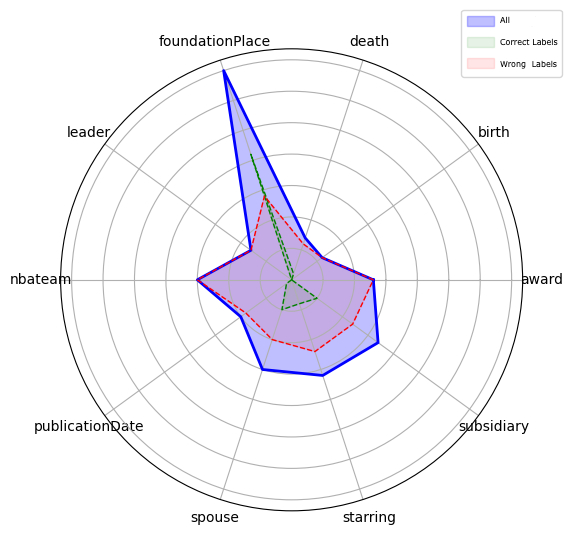
\includegraphics[width=\textwidth]{res/radar-error-1}
    \end{minipage}
    \caption{Prediction accuracy on the FactBench dataset, focusing on incorrect predictions. The left chart illustrates the Distribution of Fully Incorrect Predictions (4/4), detailing the instances where all predictions made by the model were incorrect. The right chart depicts the Distribution of Partially Incorrect Predictions (3/4).}
    \label{fig:wrong_prediction_distribution}
\end{figure}

In general, by spotting Figure~\ref{fig:wrong_prediction_distribution}, we can observe that the overall shape of the error distribution is similar, indicating consistency in the model's performance across different voting thresholds.
    \chapter{Conclusions and Future Works}\label{ch:conclusions}
\acp{LLM} show that they have changed the role of automated fact-checking, yet given the complexity and limitations of these models, while they are not 100\% accurate, it is foreseeable that they will be able to act completely as human annotators in the future.

This thesis has presented FactCheck, a novel approach to \ac{KG} fact verification using RAG.
Through extensive experimentation and analysis, we have demonstrated the effectiveness of combining multiple \acp{LLM} with sophisticated \ac{IR} techniques to verify facts in \acp{KG}.
FactCheck's prediction performance that measured against gold standard labels is 90\% on \textit{FactBench}, 87\% on \textit{YAGO}, and 70\% on \textit{DBpedia}.
These results emphasize using \acp{LLM} to address fact verification in \acp{KG}.

One of our observations is that differences in \acp{LLM} architectures make them interpret the evidence differently and reach different conclusions despite accessing the same evidence.
Additionally, another observation is the existence of particular challenges in geographic and nationality facts.
This issue points to deeper issues in how language models process contextual information, indicating that improvements in basic reasoning capabilities may prove more valuable than simple increases in model scale.

Also, in fact-verification tasks, when a binary evaluation is requested (\ie determining whether a statement is correct or incorrect), \acp{LLM} often explain when they classify a statement as incorrect.
However, when predicting a statement is correct, they typically do not explain further if not explicitly requested.

The empirical evidence challenges the conventional wisdom that larger models invariably yield better results - our experiments with embedding models and text chunking techniques demonstrate that carefully optimized smaller models can match or exceed the performance of their larger counterparts when supported by robust retrieval mechanisms.
This finding has profound implications for practical deployments, particularly in resource-constrained environments where computational efficiency is paramount.

Our analysis highlights a key challenge in current verification methods: ensemble techniques improve reliability by using consensus, but they also require a lot of computing power, which can be a problem for large-scale applications.
This suggests a critical direction for future research, the development of more efficient verification strategies that maintain accuracy while reducing computational demands.

Finally, as \acp{KG} continue to grow in importance for real-world applications, these insights provide crucial guidance for developing more efficient and reliable verification systems that balance accuracy with practical constraints.
Based on our findings and identified limitations, several promising directions for future research emerge:
\begin{enumerate}
    \item \textbf{Enhanced Context Processing:} Develop more sophisticated methods for handling cases with insufficient or irrelevant context. Implement better techniques for identifying and resolving contradictions in retrieved information.
    \item \textbf{Model Integration:} Explore additional strategies for combining model outputs beyond majority voting. Investigate dynamic model selection based on query characteristics. Implement more sophisticated tie-breaking mechanisms.
    \item \textbf{Retrieval Optimization:} Improve query generation for better coverage of fact verification requirements. Develop more effective filtering mechanisms for irrelevant information. Enhance the similarity cut-off strategy for more precise document selection.
    \item \textbf{Scalability Improvements:} Optimize computational resource usage for handling larger \acp{KG}. Develop more efficient document processing and embedding techniques. Implement parallel processing capabilities for faster verification.
    \item \textbf{Explainability and Transparency:} Develop better methods for explaining verification decisions. Implement confidence scoring mechanisms. Create visualization tools for the verification process.
    \item \textbf{Domain Adaptation:} Create specialized verification strategies for different types of facts. Develop domain-specific knowledge integration mechanisms. Implement adaptive learning capabilities for new domains.
\end{enumerate}
    \begin{appendices}
    \chapter{Prompt Templates}\label{ch:prompt-templates}
    In this section, we present the prompt templates used in the pipeline.
    \section{Human-understandable text generation Prompt}\label{sec:prompt-templates:human-understandable}
    \begin{Verbatim}[fontsize=\small, frame=single, label={Prompt template for generating human-readable text}]
Task Description:
Convert a kg triple into a meaningful human readable sentence.

Instructions:
    Given a subject, predicate, and object from a kg, form a
    grammatically correct and meaningful sentence that conveys
    the relationship between them.

Examples:
Input:
    Subject: Alexander_III_of_Russia
    Predicate: isMarriedTo
    Object:  Maria_Feodorovna__Dagmar_of_Denmark_
    Output: {"output" : "Alexander III of Russia is married to Maria
                        Feodorovna, also known as Dagmar of Denmark."}

Input:
    Subject: Quentin_Tarantino
    Predicate: produced
    Object: From_Dusk_till_Dawn
    Output: {"output": "Quentin Tarantino produced the film
                        From Dusk till Dawn."}

Input:
    Subject: Joseph_Heller
    Predicate: created
    Object: Catch-22
    Output: {"output": "Joseph Heller created the novel Catch-22."}

Do the following:
Input:
Subject: {knowledge_graph.subject}
Predicate: {knowledge_graph.predicate}
Object: {knowledge_graph.object}
The output should be a JSON object with the key "output" and
the value as the sentence. The sentence should be human-readable
and grammatically correct. The subject, predicate, and object
can be any valid string without having extra information.
    \end{Verbatim}
    \section{Question Generation Prompt}\label{sec:prompt-templates:10-question}
    \begin{Verbatim}[fontsize=\small, frame=single, label={Prompt template for generating 10 questions for each triple}]
You are an intelligent system with access to a vast amount of
information. I will provide you with a knowledge graph in the
form of triples (subject, predicate, object).

Your task is to generate ten questions based on the kg.
The questions should assess understanding and insight into the
information presented in the graph.

Provide the output in JSON format, with each question having a unique
identifier. Instructions:
 1.Analyze the provided knowledge graph.
 2.Generate ten questions that are relevant to the information in kg.
 3.Provide the questions in JSON format, each with a unique identifier.

Input Knowledge Graph: Albert Einstein bornIn Ulm, Germany
Expected Response: {
  "questions": [
    {"id": 1,
    "question": "Where was Albert Einstein born?"},
    {"id": 2,
    "question": "What is Albert Einstein known for?"},
    {"id": 3,
    "question": "In what year was the Theory of Relativity published?"},
    {"id": 4,
    "question": "Where did Albert Einstein work?"},
    {"id": 5,
    "question": "What prestigious award did Albert Einstein win?"},
    {"id": 6,
    "question": "Which theory is associated with Albert Einstein?"},
    {"id": 7,
    "question": "Which university did Albert Einstein work at?"},
    {"id": 8,
    "question": "What did Albert Einstein receive the Nobel Prize in?"},
    {"id": 9,
    "question": "In what field did Albert Einstein win a Nobel Prize?"},
    {"id": 10,
    "question": "Name the city where Albert Einstein was born."}
]}
Considering the above information, please respond to this kg: {query}
The output should be in JSON format with each question having a unique
identifier and question doesn't contain term knowledge graph, without
any additional information
    \end{Verbatim}

\chapter{Chunking Strategies}\label{ch:chunking}
    As discussed in Section~\ref{sec:chunking-strategies}, the method used to chunk input text is a critical decision in the design of a \ac{RAG} system.
    Here, we present concrete examples of how different chunking strategies affect the segmentation of text, using the \textit{correct\_spouse\_00134} entry from the FactBench dataset.
    We report the best node found by through our pipeline for each chunking strategy.
    \section{Text Splitter - Chuck Size 512}\label{sec:chunking:text-splitter}

    \section{Small2Big}\label{sec:chunking:small2big}

    \section{Sliding Window - Window Size 3}\label{sec:chunking:sliding-window}
    The knowledge graph triple \textit{correct\_award\_00000} from the FactBench dataset with triple "Henry Dunant award Nobel Peace Prize" is used as an example.
    The model used for this example is \textit{Gemma2} with \textit{similarity\_top\_k} set to 3, and \textit{BAAI/bge-small-en-v1.5} as embedding model.
    The documents are selected using \textit{ms-marco-MiniLM-L-6-v2} discussed in~\ref{subsec:supervised-methods}.
    \begin{table}[h!]
        \noindent
        \resizebox{\textwidth}{!}{
            \begin{tabular}{l}
                \toprule
                \textbf{Window} - Highlighted Text is Original Text \\
                \midrule
                \shortstack[l]{
                    You can read more about that here: From the first Nobel Prize award ceremony, 1901 \\
                    The announcement that the founder of the Red Cross had been chosen as Peace Prize \\
                    laureate met with mixed reactions. Dunant had been awarded the prize for ameliorating \\
                    the suffering of wounded soldiers, not for organising peace congresses or reducing  \\
                    standing forces, as stipulated in Alfred Nobel’s will. The Nobel Committee had chosen \\
                    a broad interpretation of the provision that a laureate should “further fraternity \\
                    between nations”. \colorbox{pink}{The Red Cross: three-time recipient of the Peace Prize Henry Dunant} \\
                    \colorbox{pink}{(1828–1910).}  Switzerland, “for his humanitarian efforts to help wounded soldiers and \\
                    create international understanding” Frédéric Passy (1822–1912).  France, “for his \\
                    lifelong work for international peace conferences, diplomacy and arbitration.”
                } \\ \hline

                \shortstack[l]{
                    On 10th of December 1901 the first Nobel Peace Prize was awarded. It went to Henry Dunant, \\
                    founder of the International Committee of the Red Cross, who shared the first Nobel Peace \\
                    Prize with Frédéric Passy, a leading international pacifist of the time. \\
                    \colorbox{pink}{Since then, the Red Cross has been awarded the Peace Prize three times.} \\
                    The Red Cross: Three-time recipient of the Peace Prize Four of them given out in Stockholm  \\
                    and one, the Peace Prize, in Christiania, as Oslo was then called. You can read more about \\
                    that here: From the first Nobel Prize award ceremony, 1901 The announcement that the founder\\
                    of the Red Cross had been chosen as Peace Prize laureate met with mixed reactions.\\
                    Dunant had been awarded the prize for ameliorating the suffering of wounded soldiers, not for \\
                    organising peace congresses or reducing standing forces, as stipulated in Alfred Nobel’s will.
                } \\ \hline
                \shortstack[l]{
                    Henry Dunant \\
                    The Nobel Peace Prize 1901 \\
                    Nobel co-recipient: Frédéric Passy \\
                    Role: Founder of the International Committee of the Red Cross, Geneva, Originator Geneva \\
                    Convention (Convention de Genève) Nobel Prize Cash and Philanthropy \\
                    Jean Henry Dunant, though poor, donated his Nobel Prize money to charity. Hans Daae, a \\
                    military physician, managed to get the money deposited in a bank in Norway. \colorbox{pink}{Thus Dunant’s}\\
                    \colorbox{pink}{creditors could not claim the money.} When Dunant was alive the money remained untouched in \\
                    the bank. He lived frugally in a Swiss nursing home. Dunant’s will bequeathed one half of \\
                    the money to the Norwegian Red Cross and the Norwegian Women’s Public Health Association.
                } \\
                \bottomrule
            \end{tabular}}\caption{Sliding Window - Window Size 3}\label{tab:table-sliding-window}
        \label{tab:table}
    \end{table}


\end{appendices}
    
    % Bibliography, appendix, acknowledges, etc...
    \backmatter
\end{document}